\clearpage

\section {Results of the $\nu_{\mu}$-disappearance analysis with the Run 1+2+3+4 %(6.5700$\times10^{20}$ POT) 
dataset}
\label{sec:results}

%--------------------------------------------------------------------------------------
% Best-fit params & pulls
%--------------------------------------------------------------------------------------

\subsection {Best-fit oscillation parameters and systematic parameter pulls}
\label{sec:results_bestfit}

Two 3-flavour $\nu_{\mu}$-disappearance fits were performed on the combined 6.5700$\times$10$^{20}$ 
POT Run 1+2+3+4 dataset, using the method described in Sec.\ \ref{sec:oscfit_method}.
In the first fit, the normal mass hierarchy was assumed, and $\sin^{2}\theta_{23}$ and $|\Delta m^{2}_{32}|$ 
were allowed to float, while, in the second fit, the inverted mass hierarchy was assumed and $\sin^{2}\theta_{23}$ 
and $|\Delta m^{2}_{31}|$ were allowed to float. In both fits, all 41 systematic parameters considered in this analysis 
and the oscillation parameters $\sin^{2}\theta_{12}$, $\sin^{2}\theta_{13}$, $\Delta m^{2}_{21}$ and $\delta_{CP}$ were 
also allowed to float. 
The best-fit values were \resultNormalMixing and \resultNormalDmsq assuming the normal mass hierarchy, 
and \resultInvertedDmsq and \resultInvertedMixing assuming the inverted mass hierarchy. 

An identical analysis was also carried out separately on both the 3.0100$\times$10$^{20}$ POT Run 1+2+3 and
3.5600$\times$10$^{20}$ POT Run 4 datasets for the normal mass hierarchy only.
Similar best-fit values were obtained from these fits of subsets of the full dataset. 
The fit to the Run 1+2+3 dataset gave best-fit values of 
\resultNormalRunITIIIMixing and \resultNormalRunITIIIDmsq
while a fit to the Run 4 dataset gave 
\resultNormalRunIVMixing and \resultNormalRunIVDmsq.

The results of these fits are summarized in Tab.\ \ref{tab:data_fits:best_fit_values}. In this table are 
the best-fit oscillation parameters, the observed and expected numbers of single $\mu$-like ring events,
and the values of $\chi^{2}$ per degree of freedom at the best fit.

The pull for each systematic parameter $f$ included in the fit was calculated as
\begin{equation}
  \frac{f_{bestfit} - f_{nom}}{\sigma},
\end{equation}
where 
$f_{bestfit}$ is the best-fit value of the systematic parameter,
$f_{nom}$ is the nominal value of the parameter (corresponding to no systematic variation), and
$\sigma$ is either $\sigma_{input}$ (the prefit error)\footnote{For $\delta_{CP}$, $\sigma_{input}$ is taken to be $\pi$.} 
or $\sigma_{bestfit}$ (the Hesse error output from Minuit).

The pulls of all 45 nuisance parameters allowed to float in these fits are shown in 
Figs.\ \ref{fig:results_data1234_pulls:normal} and \ref{fig:results_data1234_pulls:inverted} 
assuming the normal and inverted mass hierarchies respectively.
% , and in 
% Figs.\ \ref{fig:results_data123_pulls}-\ref{fig:results_data4_pulls} for the
% fits to the Run 1+2+3 and Run 4 datasets.
From these figures, it is apparent that most systematic parameters barely move from their nominal values.
We note that, although all 45 nuisance parameters are allowed to float in the fit,
only \resultNormalLargePulls(\resultInvertedLargePulls) of them move by more than $\pm$0.1$\sigma_{bestfit}$ for 
the normal(inverted) hierarchy fit. When a systematic parameter that is free to move stays close to its nominal 
value, it means that the reduction in $\chi^{2}$ from moving that parameter is less than the corresponding increase 
in the penalty term defined in Eq.\ \ref{eq:chisquare} in Sec.\ \ref{sec:oscfit_method}.
%equation 3 in Sec.\ 4.1.5 in Ref.\ \cite{OurRun123DisappAnalysis3Flavour}). 
Only certain systematics are able to change the predicted reconstructed energy spectrum to a 
sufficient extent to offset the penalty term. 

%...........................................................
%
% Table summarizing best-fit results
%
\begin{table}[htb]
\centering
\begin{tabular}{| l | l | c | c | c  c | c | c |}
\hline
Analysis & Run period & $\sin^{2}\theta_{23}$ & $\Delta m^2$ & N$_{obs}$ & N$_{exp}$ & $\chi^2_{bf} / ndf$ & p-value \\
\hline
2013 3-flavour Normal   & Run 1+2+3+4 & \resultNormalMixingNumber &  \resultNormalDmsqNumber $\cdot 10^{-3}$
& \NskObserved & \resultNormalNevents & \resultNormalChisq & \resultNormalPvalue \\
2013 3-flavour Inverted   & Run 1+2+3+4 & \resultInvertedMixingNumber &  \resultInvertedDmsqNumber $\cdot 10^{-3}$
& \NskObserved & \resultInvertedNevents & \resultInvertedChisq & \resultInvertedPvalue \\
2013 3-flavour Normal & Run 4        & \resultNormalRunITIIIMixingNumber &  \resultNormalRunITIIIDmsqNumber $\cdot 10^{-3}$
& 61 & \resultNormalRunITIIINevents & \resultNormalRunITIIIChisq & \resultNormalRunITIIIPvalue \\
2013 3-flavour Normal & Run 1+2+3    & \resultNormalRunIVMixingNumber &  \resultNormalRunIVDmsqNumber $\cdot 10^{-3}$
& 59 & \resultNormalRunIVNevents & \resultNormalRunIVChisq & \resultNormalRunIVPvalue \\
2012 3-flavour Normal & Run 1+2+3    & 0.514 &  2.44 $\cdot 10^{-3}$ & 58 & 57.97 & 56.04/71 & 0.83 \\
\hline
\end{tabular}
\caption{
  Summary of best-fit parameters from the fits of the Run 1+2+3, Run 4, and combined Run 1+2+3+4 datasets.
  In this table, $\Delta m^2$ is $|\Delta m^2_{32}|$ for normal hierarchy, and $|\Delta m^2_{31}|$ for inverted hierarchy.
  The 2012 result is taken from the analysis presented in \cite{OurRun123DisappAnalysis3Flavour}
  (note that the difference in N$_{obs}$ between 2012 and 2013 for the Run 1+2+3 dataset is due to a reanalysis of the data \cite{SuperkEScale2013}).
  The quoted best-fit $\chi^2$ values ($\chi^2_{bf}$) were computed from Eq.\ \ref{eq:chisquare} in Sec.\ \ref{sec:oscfit_method}.
  using the reconstructed energy binning scheme given in Sec.\ \ref{sec:mc_templates:template_binning}.
  The table also shows the p-values obtained from the goodness-of-fit test described in Sec.\ \ref{sec:gof_test}
  for all fits.
}
\label{tab:data_fits:best_fit_values}
\end{table}

%...........................................................
%
% Systematic parameter pulls 
%

\begin{figure*}[htb]
\center
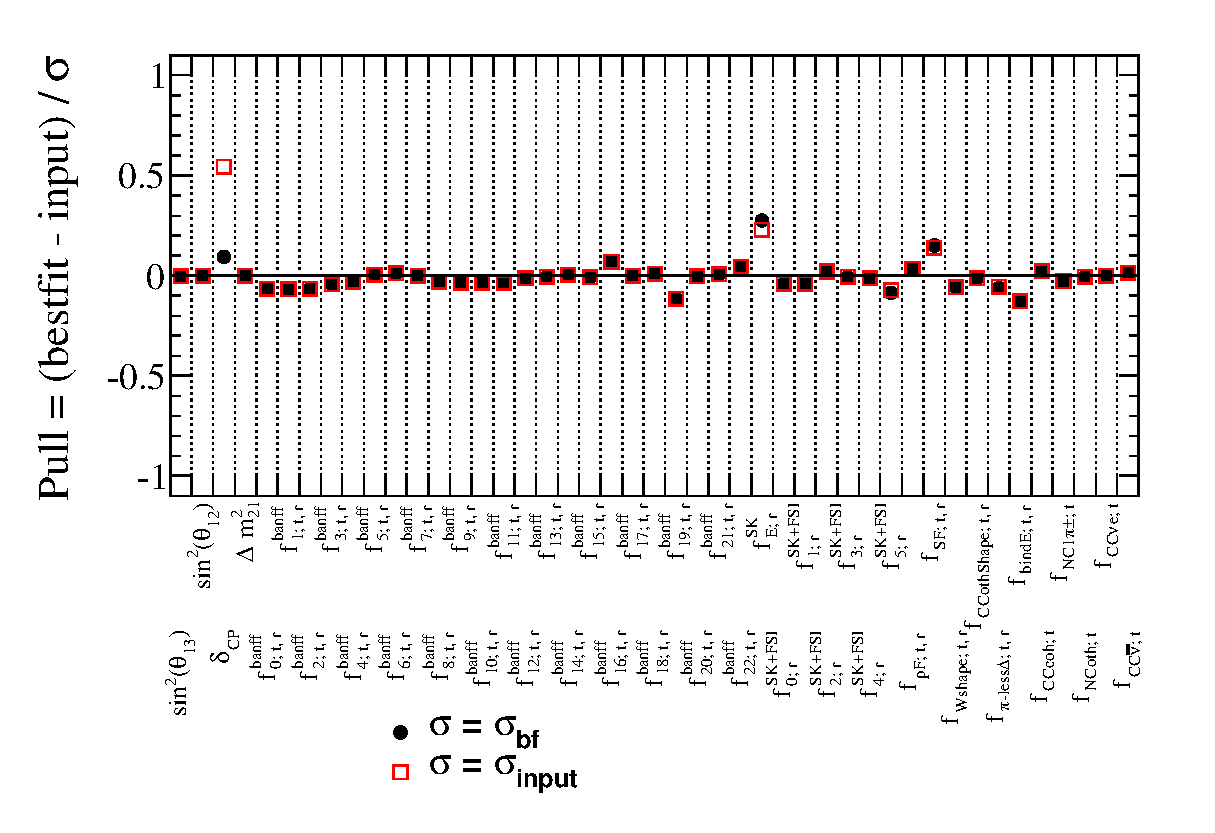
\includegraphics[width=50pc,angle=270]{./images/data_fit/normal/run1-4_nuis4_sintheta_normal_pulls_and_values}
\caption {
  Systematic parameter pulls from the fit of the Run 1+2+3+4 dataset.
  The normal mass hierarchy is assumed.
}
\label{fig:results_data1234_pulls:normal}
\end{figure*}

\begin{figure*}[htb]
\center
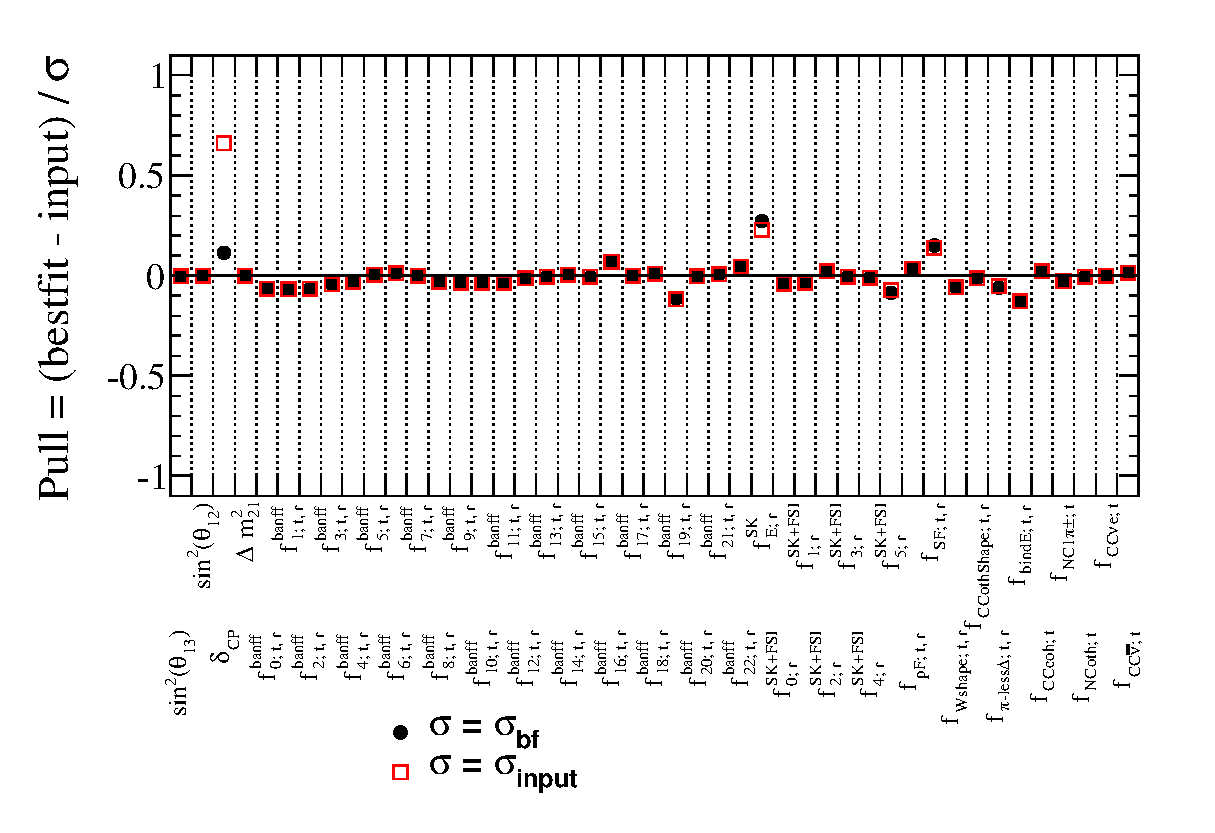
\includegraphics[width=50pc,angle=270]{./images/data_fit/inverted31/run1-4_nuis4_sintheta_inverted31_pulls_and_values}
\caption {
  Systematic parameter pulls from the fit of the Run 1+2+3+4 dataset.
  The inverted mass hierarchy is assumed.
}
\label{fig:results_data1234_pulls:inverted}
\end{figure*}

\begin{figure*}[htb]
  \begin{minipage}[t]{0.48\linewidth}
    \center
    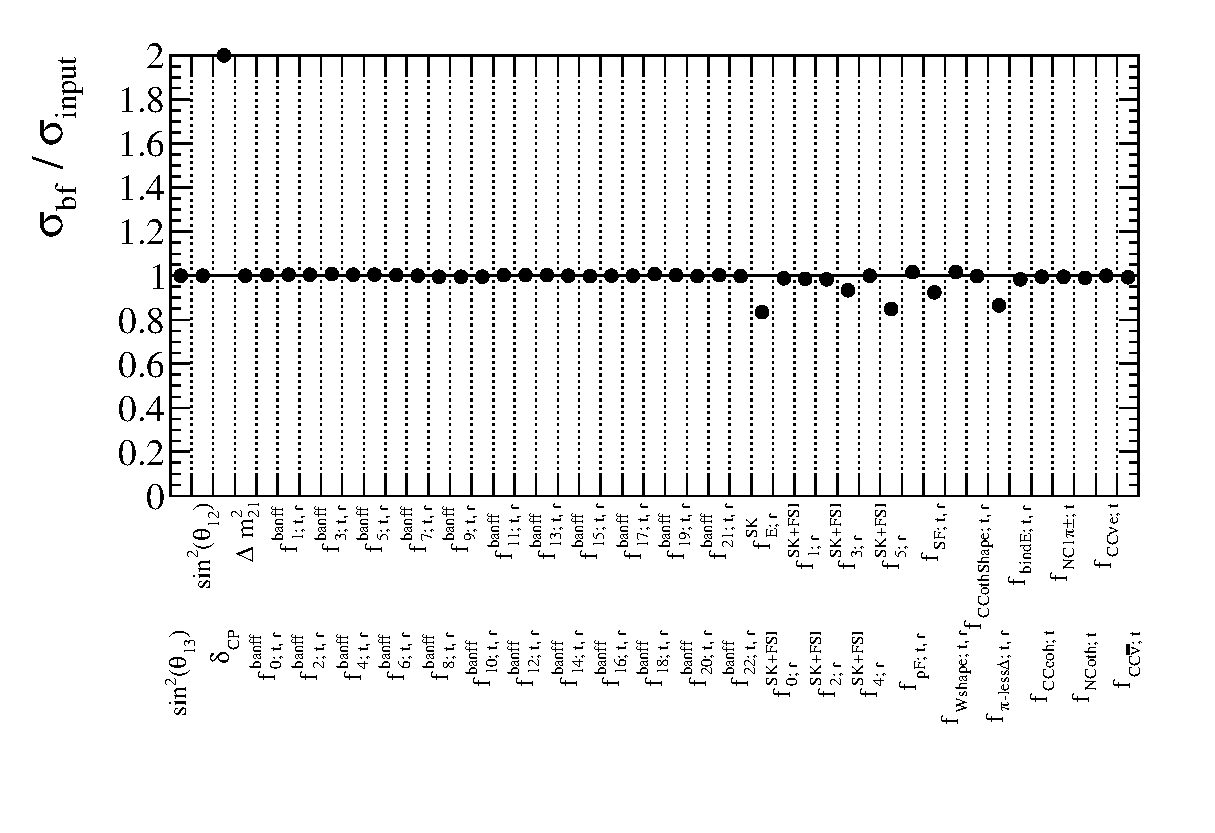
\includegraphics[width=28pc,angle=270]{./images/data_fit/normal/run1-4_nuis4_sintheta_normal_err_ratio}
    \caption {
      Ratio of $\sigma_{bestfit}$ / $\sigma_{input}$ from the fit of the Run 1+2+3+4 dataset.
      The normal mass hierarchy is assumed.
    }
    \label{fig:results_data1234_errratio:normal}
  \end{minipage}
  \hspace{0.06\linewidth}
  \begin{minipage}[t]{0.48\linewidth}
    \center
    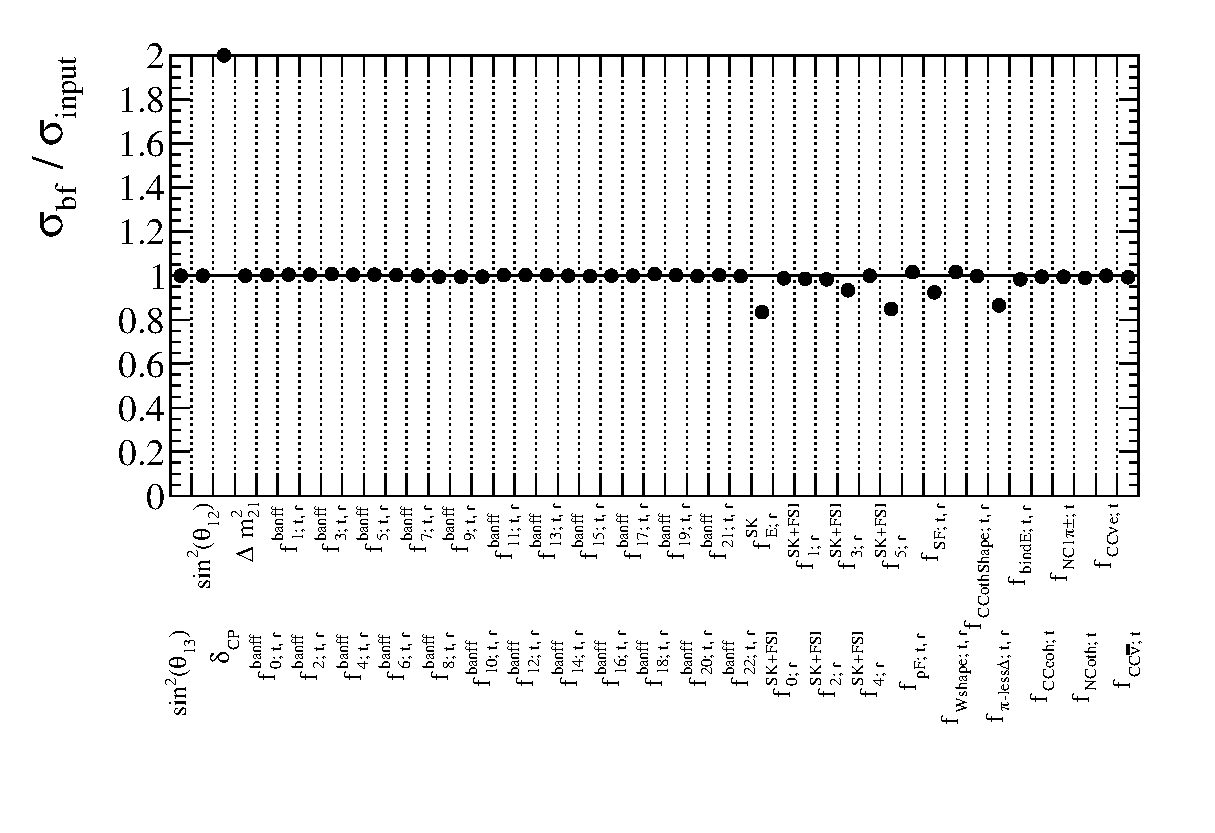
\includegraphics[width=28pc,angle=270]{./images/data_fit/inverted31/run1-4_nuis4_sintheta_inverted31_err_ratio}
    \caption {
      Ratio of $\sigma_{bestfit}$ / $\sigma_{input}$ from the fit of the Run 1+2+3+4 dataset.
      The inverted mass hierarchy is assumed.
    }
    \label{fig:results_data1234_errratio:inverted}
  \end{minipage}
\end{figure*}

%--------------------------------------------------------------------------------------
% Goodness of fit tests
%--------------------------------------------------------------------------------------

\subsection {Goodness-of-fit tests}
\label{sec:results_gof}

Goodness-of-fit tests were performed as described in Sec.\ \ref{sec:gof_test}, %\ 4.2 of Ref. \cite{OurRun123DisappAnalysis3Flavour},
and the p-values from the fits of the Run 1+2+3+4 dataset %, Run 1+2+3 and Run 4 datasets
are shown in Tab.\ \ref{tab:data_fits:best_fit_values}. 
The $\chi^2$ distributions from which these p-values were calculated are shown for the 
Run 1+2+3+4 data in Figs.\ \ref{fig:results_data1234_goodness:normal} and \ref{fig:results_data1234_goodness:inverted}
for the normal and inverted mass hierarchies respectively.
Both %All
fits have a high degree of plausibility.

%..................................
%
% Chisq_{gof} distributions
% 

\begin{figure*}[htb]
  \centering{
    \begin{minipage}[t]{0.8\linewidth}
      \center
      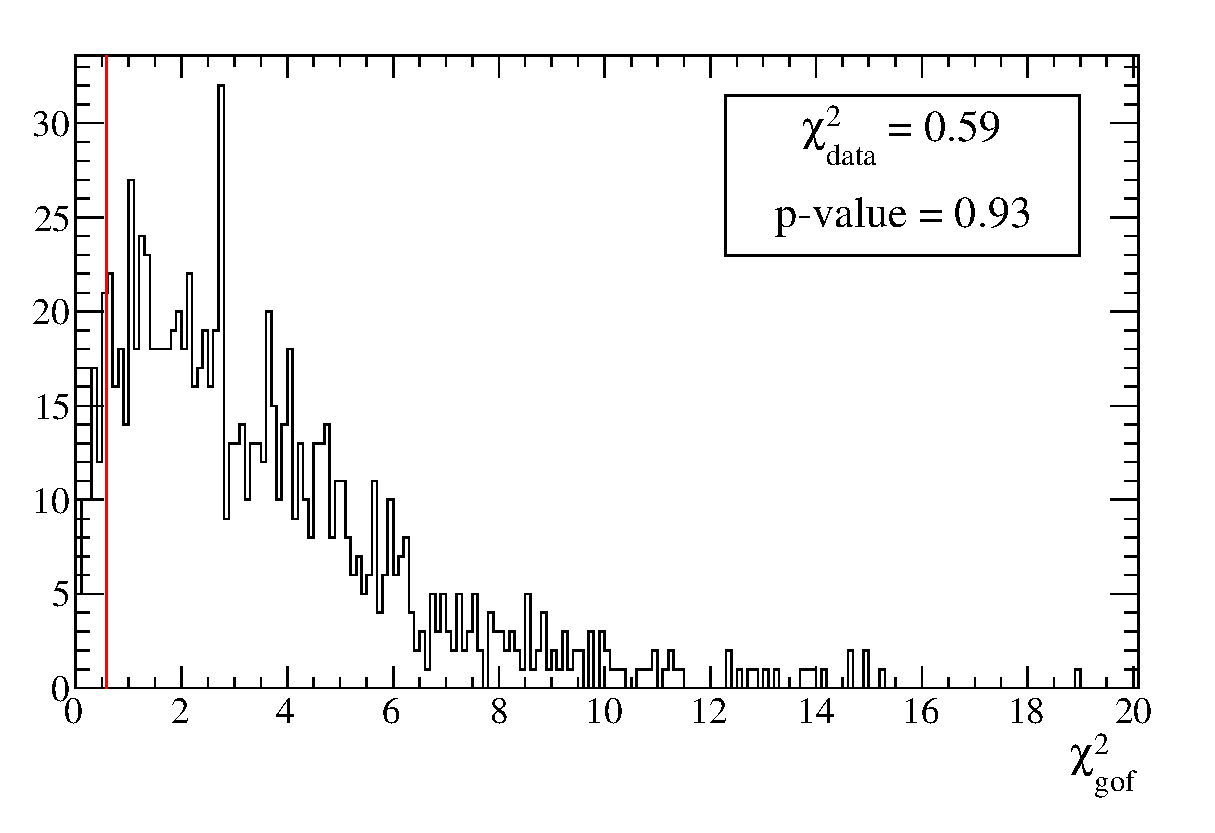
\includegraphics[width=24pc]{./images/data_fit/normal/goodness_run1-4_nuis4_sintheta_normal}
      \caption {
        Distribution of $\chi^2_{gof}$, the goodness-of-fit (gof) $\chi^2$, 
        from 1k toy MC experiments whose true input values were the Run 1+2+3+4 best-fit oscillation parameters.
        The $\chi^2_{gof}$ value from the fit of the Run 1+2+3+4 data ($\chi^2_{data}$) is highlighted.
        The normal mass hierarchy is assumed.
      }
      \label{fig:results_data1234_goodness:normal}
    \end{minipage}
    \vfill
    \begin{minipage}[t]{0.8\linewidth}

      \center
      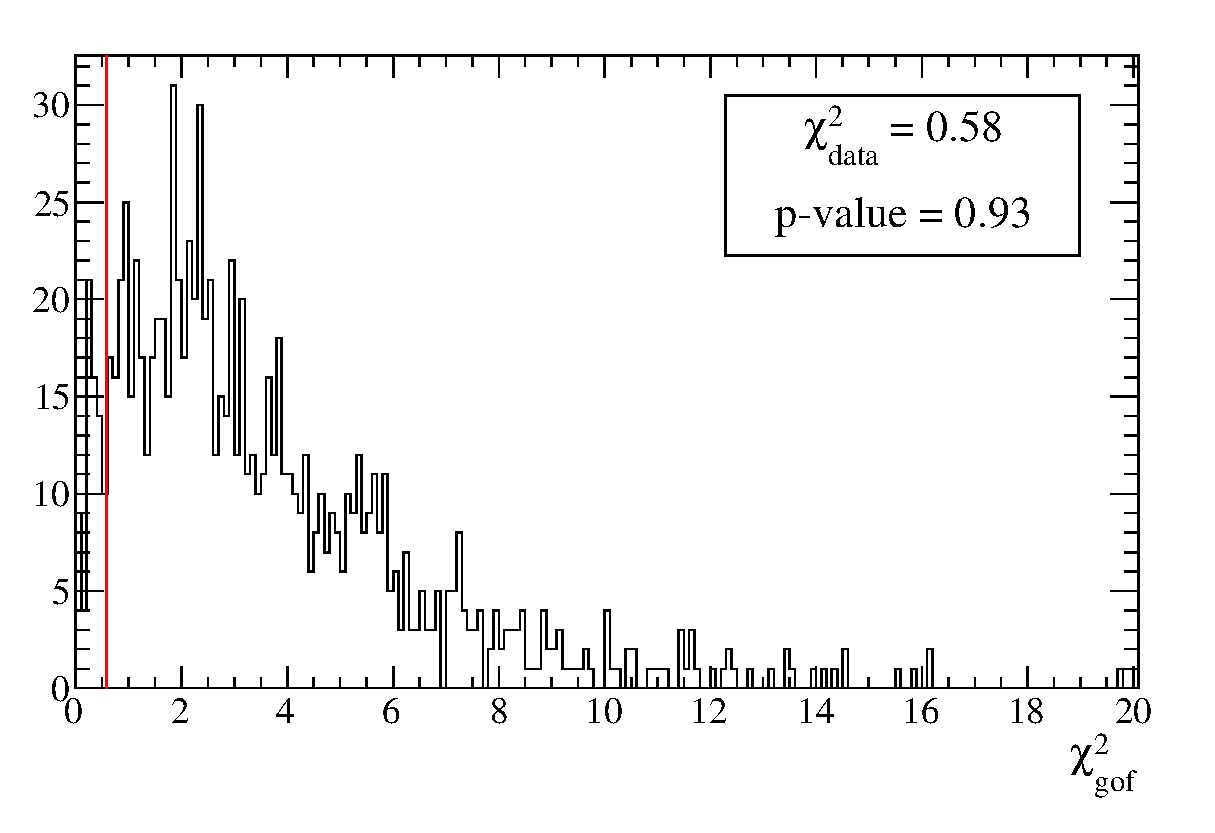
\includegraphics[width=24pc]{./images/data_fit/inverted31/goodness_run1-4_nuis4_sintheta_inverted31}
      \caption {
        Distribution of $\chi^2_{gof}$, the goodness-of-fit (gof) $\chi^2$, 
        from 1k toy MC experiments whose true input values were the Run 1+2+3+4 best-fit oscillation parameters.
        The $\chi^2_{gof}$ value for the fit of the Run 1+2+3+4 data ($\chi^2_{data}$) is highlighted.
        The inverted mass hierarchy is assumed.
      }
      \label{fig:results_data1234_goodness:inverted}
    \end{minipage}
  }
\end{figure*}


%--------------------------------------------------------------------------------------
% Best-fit spectra
%--------------------------------------------------------------------------------------

\subsection {Best-fit single-ring $\mu$-like reconstructed energy spectra}
\label{sec:results_bestfit_spectra}

The reconstructed neutrino energy distribution of the single $\mu$-like ring events in the Run 1+2+3+4 dataset 
is shown in Fig.\  \ref{fig:results_data1234_spectrum:normal} along with the best-fit predicted spectrum assuming 
the normal mass hierarchy and the predicted spectrum under the no-oscillation hypothesis. Also shown is the ratio of 
the data to the no-oscillation spectrum and the ratio of the best-fit spectrum to the no-oscillation spectrum; 
in both of these ratios, the characteristic energy-dependent deficit can be clearly seen.
The corresponding spectra for the fit assuming the inverted mass hierarchy are shown in Fig.\ \ref{fig:results_data1234_spectrum:inverted}.
The equivalent spectra for the Run 1+2+3 and Run 4 datasets are also shown in 
Figs.\ \ref{fig:results_data123_spectrum} and \ref{fig:results_data4_spectrum} respectively. 
All these distributions are shown in the 73-bin scheme in reconstructed 
neutrino energy that was used in the fitting procedure (see Sec.\ \ref{sec:mc_templates:template_binning}).

Since the reconstructed energy binning used in the fit is relatively fine, it can be beneficial to see the above distributions using 
a coarser binning. The best-fit spectra obtained from the fits of the Run 1+2+3+4 %, Run 1+2+3 and Run 4 datasets are
dataset are 
shown using a coarser binning scheme\footnote{
  16 reconstructed energy bins arranged as follows:
  1 0.3-GeV bin from 0 - 0.3 GeV,
  8 0.1-GeV bins from 0.3 - 1.1 GeV,
  1 0.15-GeV bin from 1.1 GeV - 1.25 GeV,
  1 0.25-GeV bin from 1.25 - 1.5 GeV GeV,
  1 0.5-GeV bin from 1.5 - 2 GeV,
  2 1-GeV bin from 2-4 GeV,
  1 2-GeV bin from 4-6 GeV and
  1 bin above 6 GeV.
} 
in Figs.\
\ref{fig:results_data1234_spectrum_coarse:normal} and \ref{fig:results_data1234_spectrum_coarse:inverted}
for the normal and inverted mass hierarchies respectively. The best-fit spectra from the fits of 
the Run 1+2+3 and Run 4 datasets are also shown in Figs.\
\ref{fig:results_data123_spectrum_coarse} and
\ref{fig:results_data4_spectrum_coarse} respectively. 
It is interesting to see the components of the best-fit predicted spectrum, and these are shown in
Figs.\ \ref{fig:results_data1234_spectrum_components:normal} and \ref{fig:results_data1234_spectrum_components:inverted}
for the normal and inverted mass hierarchies respectively.
In these plots, the 32 components of the predicted spectrum are grouped into 5 categories: 
$\nu_{\mu}$ CCQE, $\nu_{\mu}$ CCnonQE, $\bar{\nu}_{\mu}$ CC, $\nu_{e}$/$\bar{\nu}_{e}$ CC and NC (though each of the 32 
components is calculated separately in the actual analysis).

The best-fit predicted spectra for the normal and inverted mass hierarchies are compared for the Run 1+2+3+4 dataset in
Fig.\ \ref{fig:results_data1234_spectrum_comparison},
using the 73 reconstructed energy bins used in the fit, and in
Fig. \ref{fig:results_data1234_spectrum_comparison_coarse},
using the coarser binning described above.
These two best-fit spectra are nearly identical.

Finally, the best-fit predicted spectra for the Run 1+2+3, Run 4, and Run 1+2+3+4 datasets,
all scaled to Run 1+2+3+4 POT, are compared for
the normal mass hierarchy in 
Fig.\ \ref{fig:results_dataruns_spectrum_comparison},
using the 73 reconstructed energy bins used in the fit, and in
Fig. \ref{fig:results_dataruns_spectrum_comparison_coarse},
using the coarser binning described above.
The spectra are consistent;
the largest differences below the oscillation maximum are consistent with a shift in $|\Delta m^2_{32}|$.

% {\color{red} We could also show a comparison between the 5 components listed above 
% and, also, show results of a test to check consistency between the 3 best-fit predictions}.

%...........................................................
%
% Best-fit spectra and ratios (73 bins)
%
\begin{figure*}[htb]
  \centering{
    \begin{minipage}[t]{0.8\linewidth}
      \center
      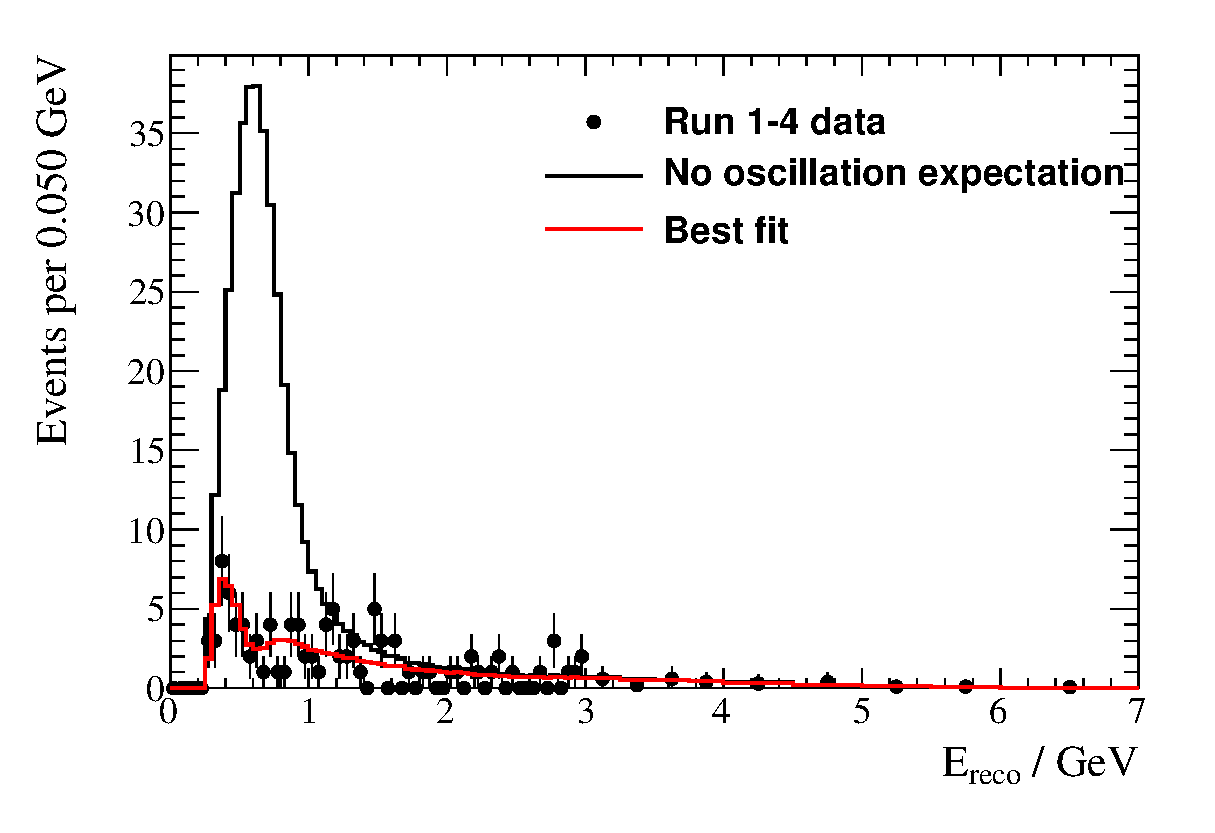
\includegraphics[width=28pc]{./images/data_fit/normal/run1-4_nuis4_sintheta_normal_spectrumper50}
    \end{minipage}
    \vfill
    \begin{minipage}[t]{0.8\linewidth}
      \center
      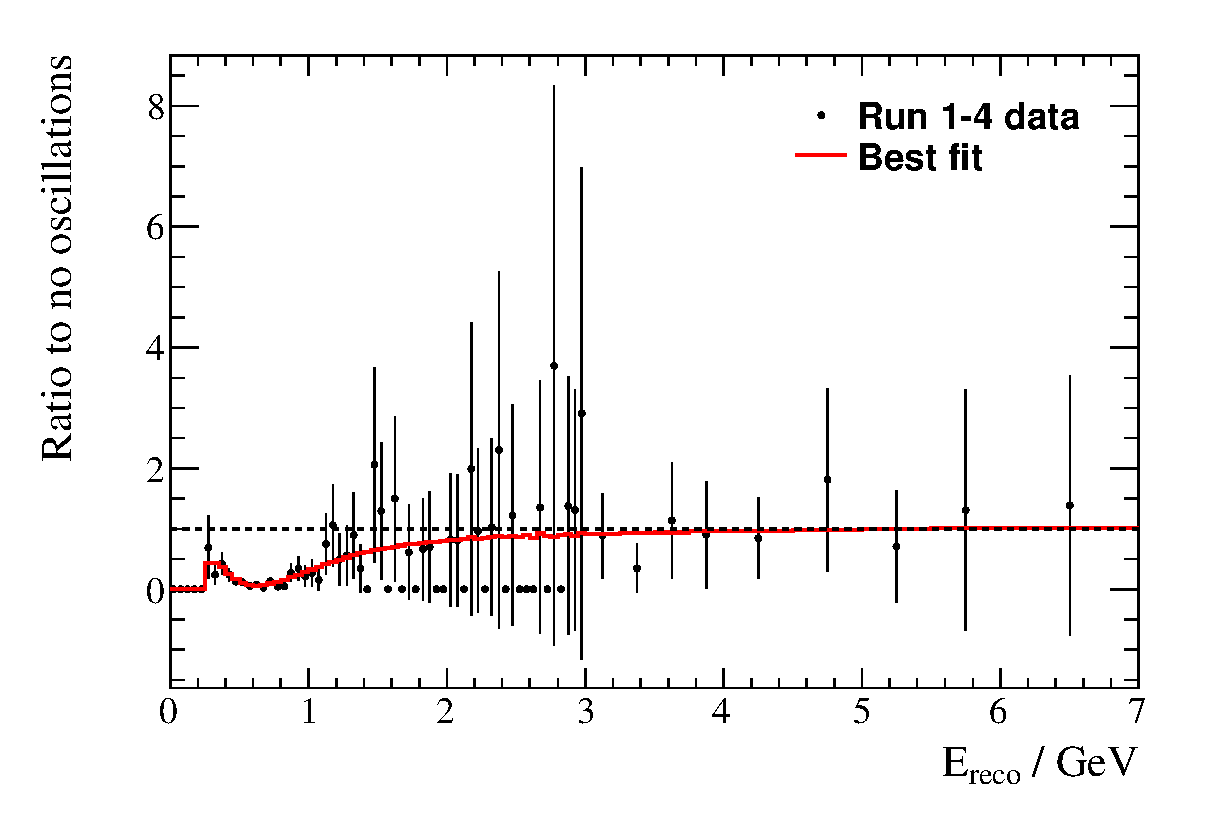
\includegraphics[width=28pc]{./images/data_fit/normal/run1-4_nuis4_sintheta_normal_spectrum_ratio}
    \end{minipage}
    \caption {
      Best-fit reconstructed energy spectrum (top) obtained from the fit of the combined Run 1+2+3+4 dataset.
      The Run 1+2+3+4 data and the prediction obtained using the no-oscillation hypothesis are also shown.
      The spectra are shown using the 73 bins used in the fit (see Sec.\ \ref{sec:mc_templates:template_binning}).
      The ratios of the data and best-fit predicted spectrum to the no-oscillation hypothesis are shown 
      in the lower plot. The characteristic energy-dependent deficit can be clearly seen.
      The normal mass hierarchy is assumed.
      \label{fig:results_data1234_spectrum:normal}
    }
  }
\end{figure*}

\begin{figure*}[htb]
  \centering{
    \begin{minipage}[t]{0.8\linewidth}
      \center
      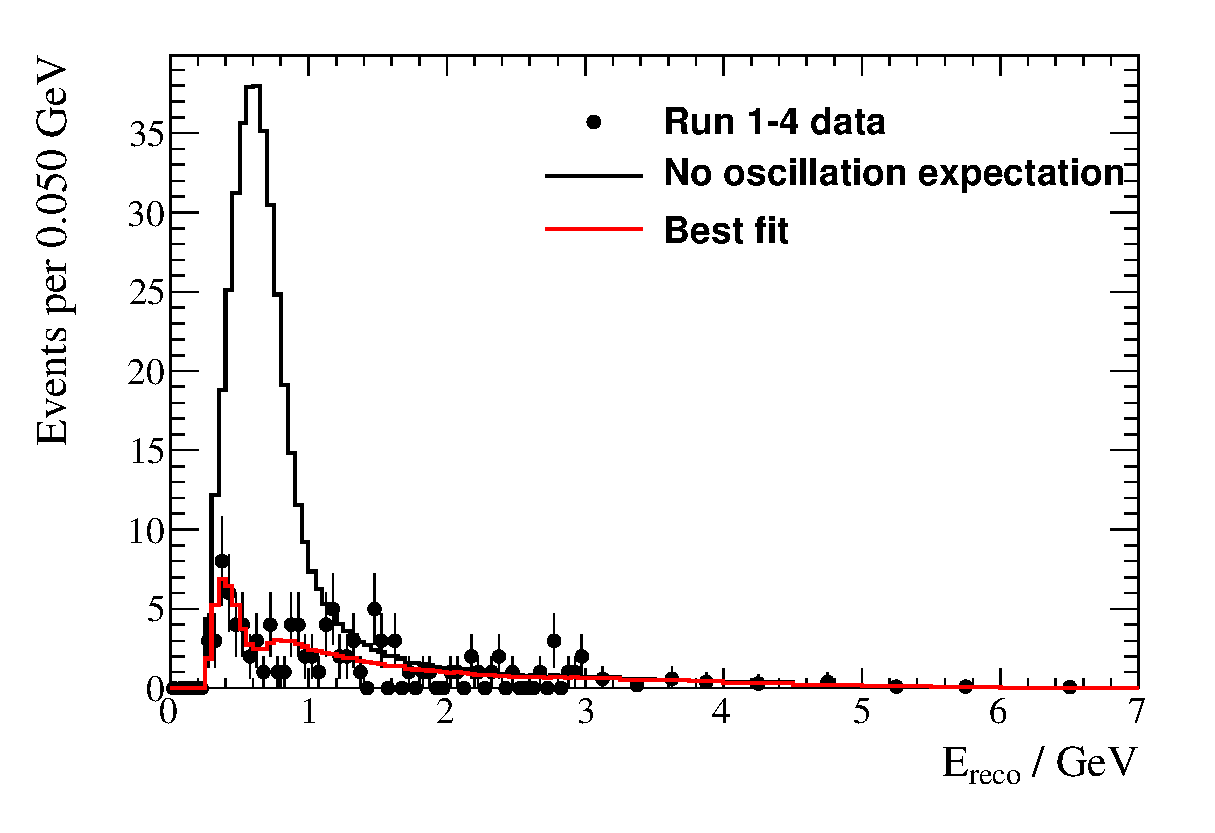
\includegraphics[width=28pc]{./images/data_fit/inverted31/run1-4_nuis4_sintheta_inverted31_spectrumper50}
    \end{minipage}
    \vfill
    \begin{minipage}[t]{0.8\linewidth}
      \center
      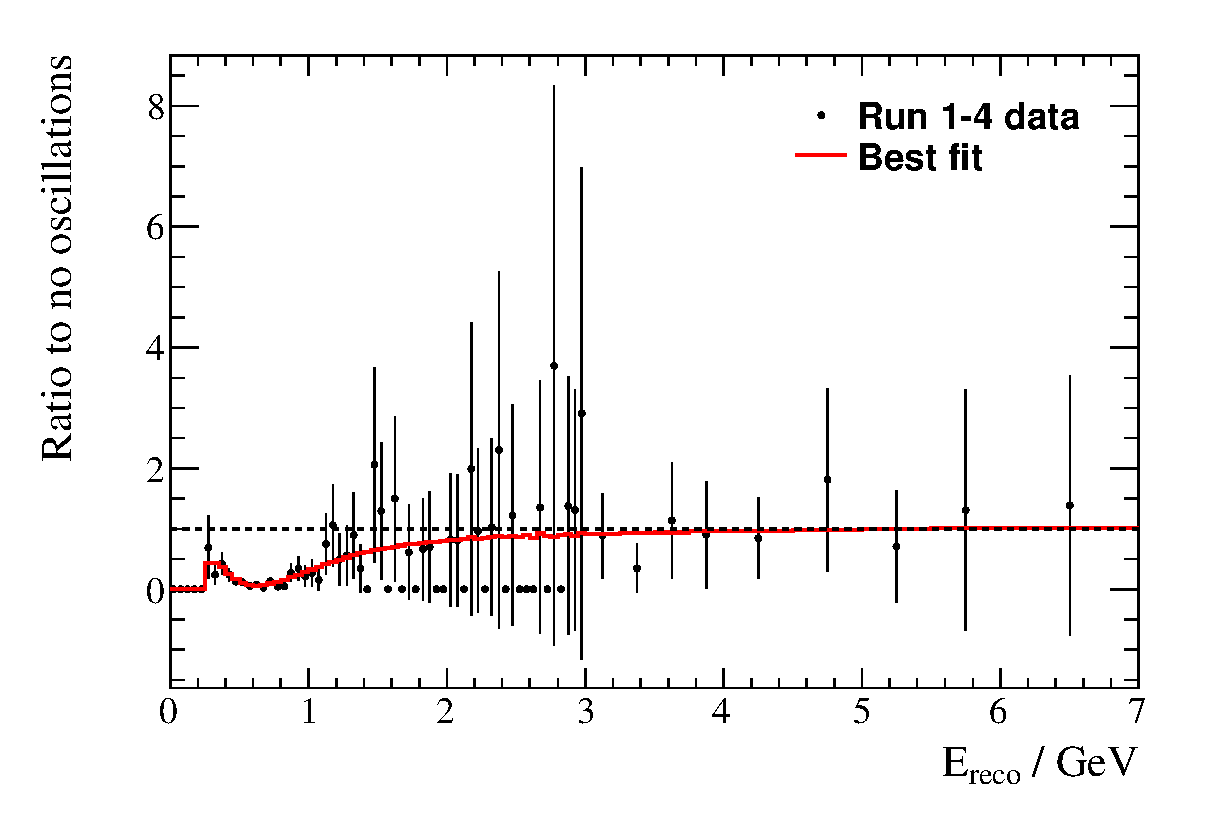
\includegraphics[width=28pc]{./images/data_fit/inverted31/run1-4_nuis4_sintheta_inverted31_spectrum_ratio}
    \end{minipage}
    \caption {
      Best-fit reconstructed energy spectrum (top) obtained from the fit of the combined Run 1+2+3+4 dataset.
      The Run 1+2+3+4 data and the prediction obtained using the no-oscillation hypothesis are also shown.
      The spectra are shown using the 73 bins used in the fit (see Sec.\ \ref{sec:mc_templates:template_binning}).
      The ratios of the data and best-fit predicted spectrum to the no-oscillation hypothesis are shown 
      in the lower plot. The characteristic energy-dependent deficit can be clearly seen.
      The inverted mass hierarchy is assumed.
      \label{fig:results_data1234_spectrum:inverted}
    }
  }
\end{figure*}

\begin{figure*}[htb]
  \begin{minipage}[t]{0.48\linewidth}
    \center
    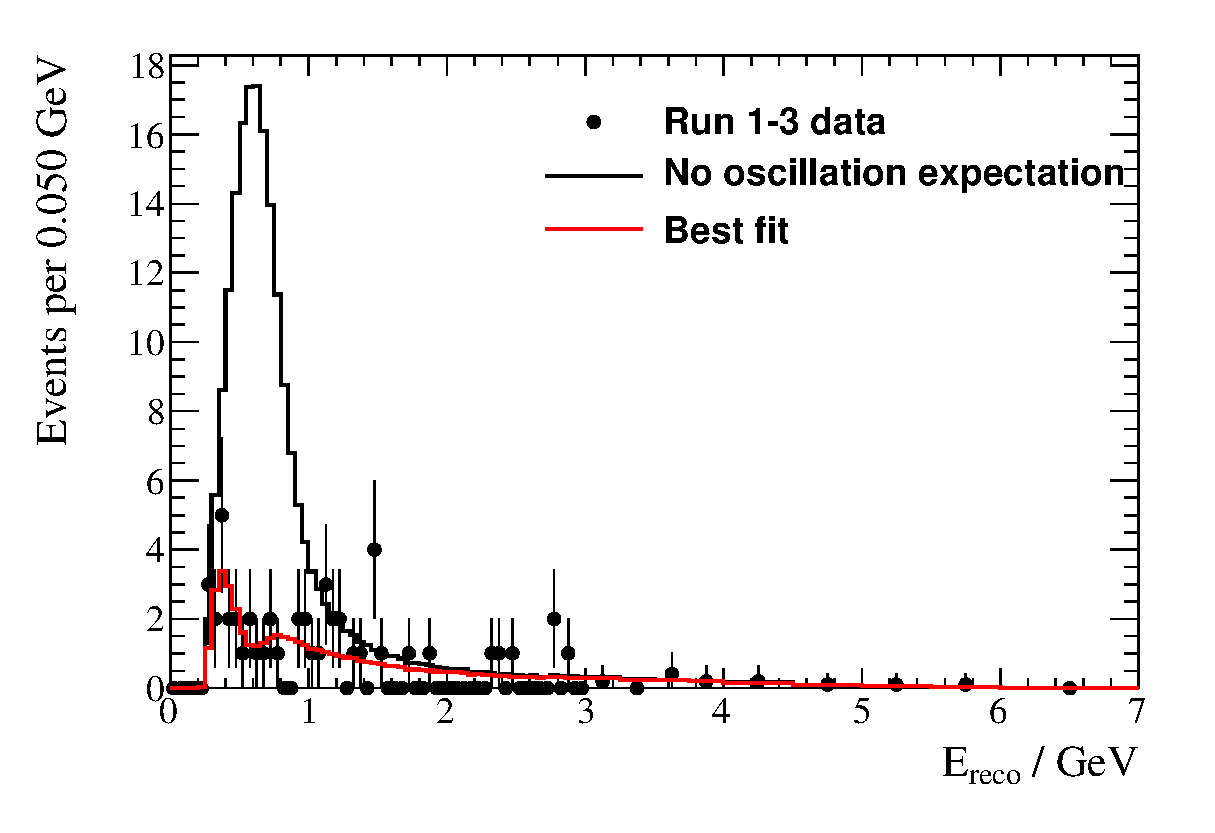
\includegraphics[width=20pc]{./images/data_fit/run123/run1-4_nuis4_sintheta_normal_run123_spectrumper50}
  \end{minipage}
  \hspace{0.06\linewidth}
  \begin{minipage}[t]{0.48\linewidth}
    \center
    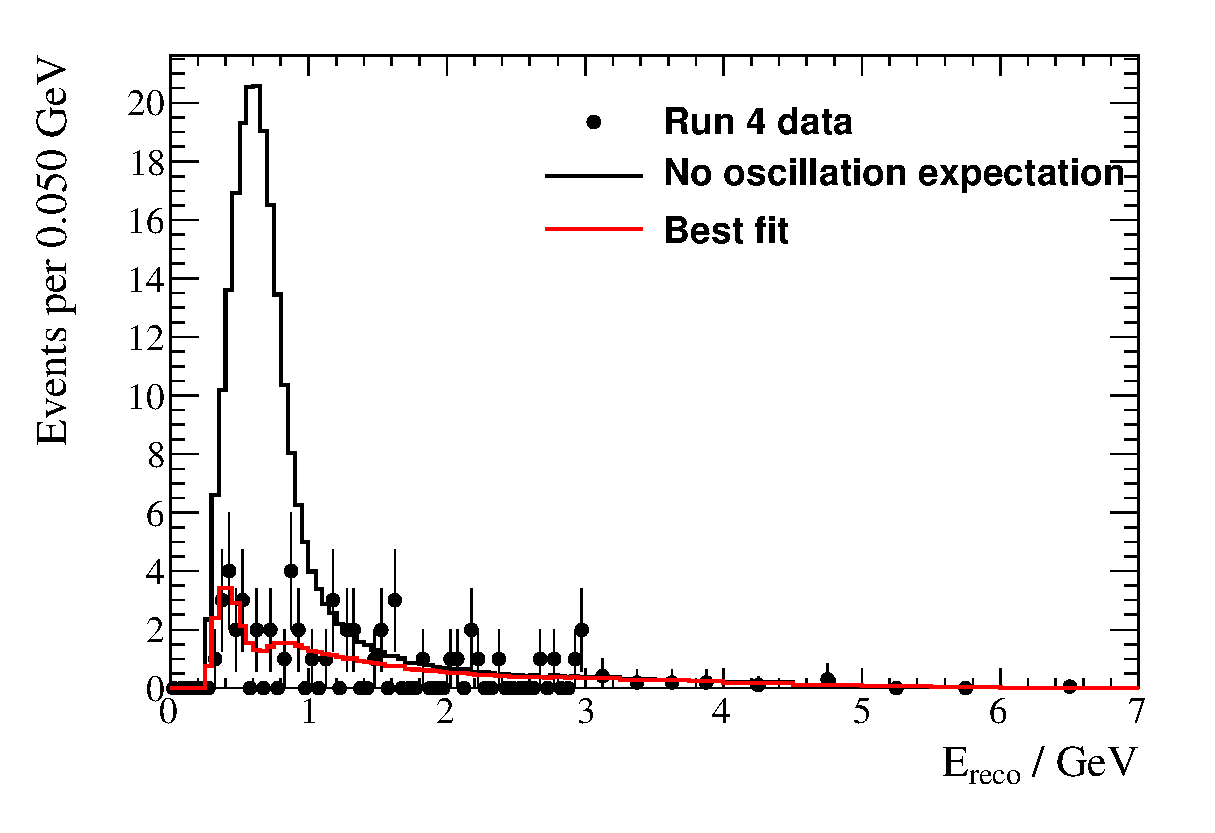
\includegraphics[width=20pc]{./images/data_fit/run4/run1-4_nuis4_sintheta_normal_run4_spectrumper50}
  \end{minipage}
  \vfill
  \begin{minipage}[t]{0.48\linewidth}
    \center
    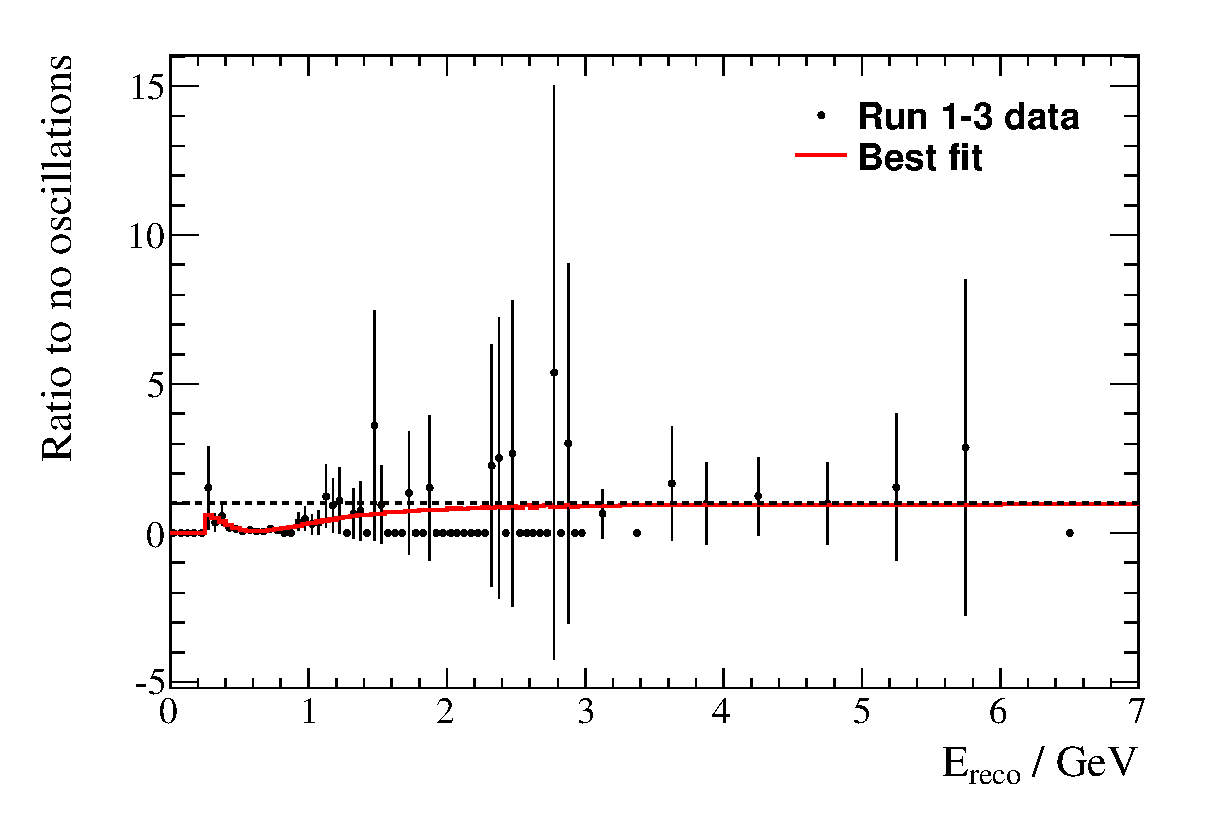
\includegraphics[width=20pc]{./images/data_fit/run123/run1-4_nuis4_sintheta_normal_run123_spectrum_ratio}
    \caption {
      Best-fit reconstructed energy spectrum (top) obtained from the fit of the Run 1+2+3 dataset only.
      The Run 1+2+3 data and the prediction obtained using the no-oscillation hypothesis are also shown.
      The spectra are shown using the 73 bins used in the fit (see Sec.\ \ref{sec:mc_templates:template_binning}).
      The ratios of the data and best-fit predicted spectrum to the no-oscillation hypothesis are shown
      in the lower plot. The characteristic energy-dependent deficit can be clearly seen.
      The normal mass hierarchy is assumed.
    }
    \label{fig:results_data123_spectrum}
  \end{minipage}
  \hspace{0.06\linewidth}
  \begin{minipage}[t]{0.48\linewidth}
    \center
    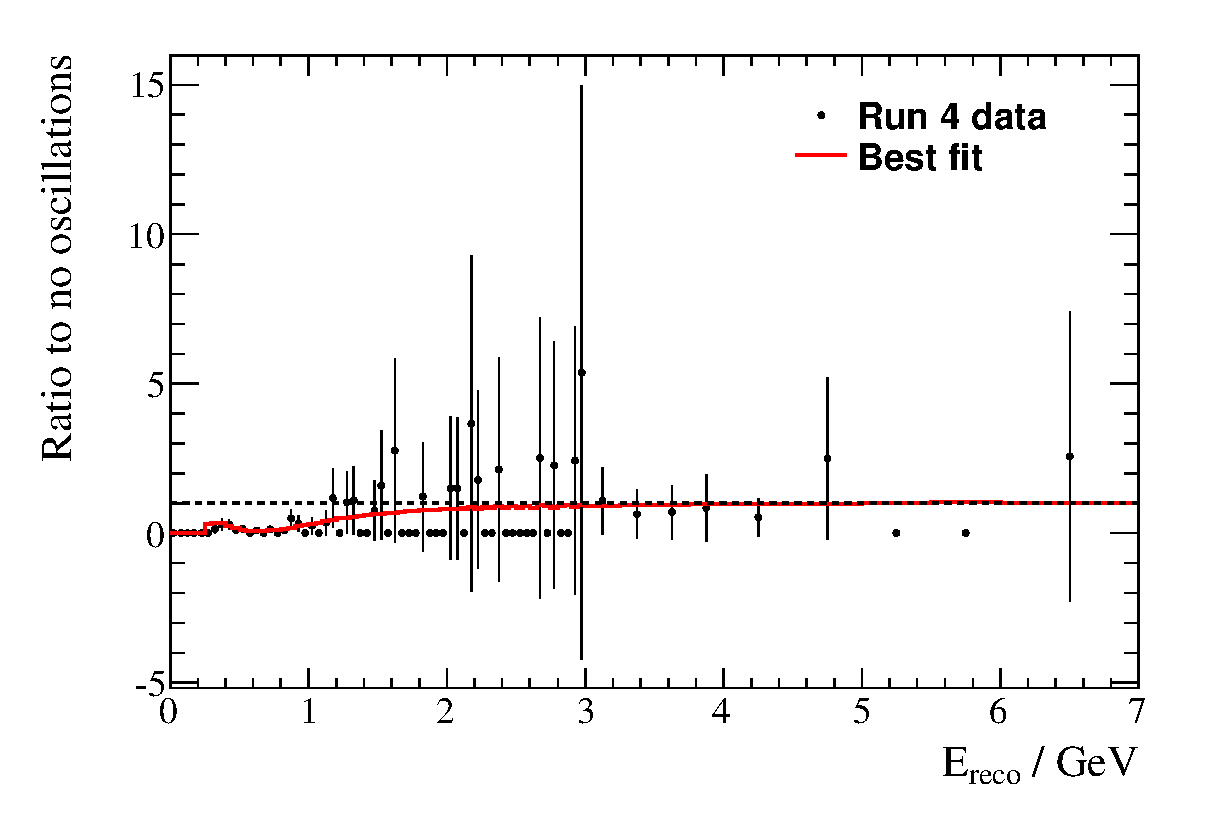
\includegraphics[width=20pc]{./images/data_fit/run4/run1-4_nuis4_sintheta_normal_run4_spectrum_ratio}
    \caption {
      Best-fit reconstructed energy spectrum (top) obtained from the fit of the combined Run 4 dataset only.
      The Run 4 data and the prediction obtained using the no-oscillation hypothesis are also shown.
      The spectra are shown using the 73 bins used in the fit (see Sec.\ \ref{sec:mc_templates:template_binning}).
      The ratios of the data and best-fit predicted spectrum to the no-oscillation hypothesis are shown
      in the lower plot. The characteristic energy-dependent deficit can be clearly seen.
      The normal mass hierarchy is assumed.
    }
    \label{fig:results_data4_spectrum}
  \end{minipage}
\end{figure*}

%...........................................................
%
% Best-fit spectra and ratios (coarse binning)
%
\begin{figure*}[htb]
  \centering{
    \begin{minipage}[t]{0.8\linewidth}
      \center
      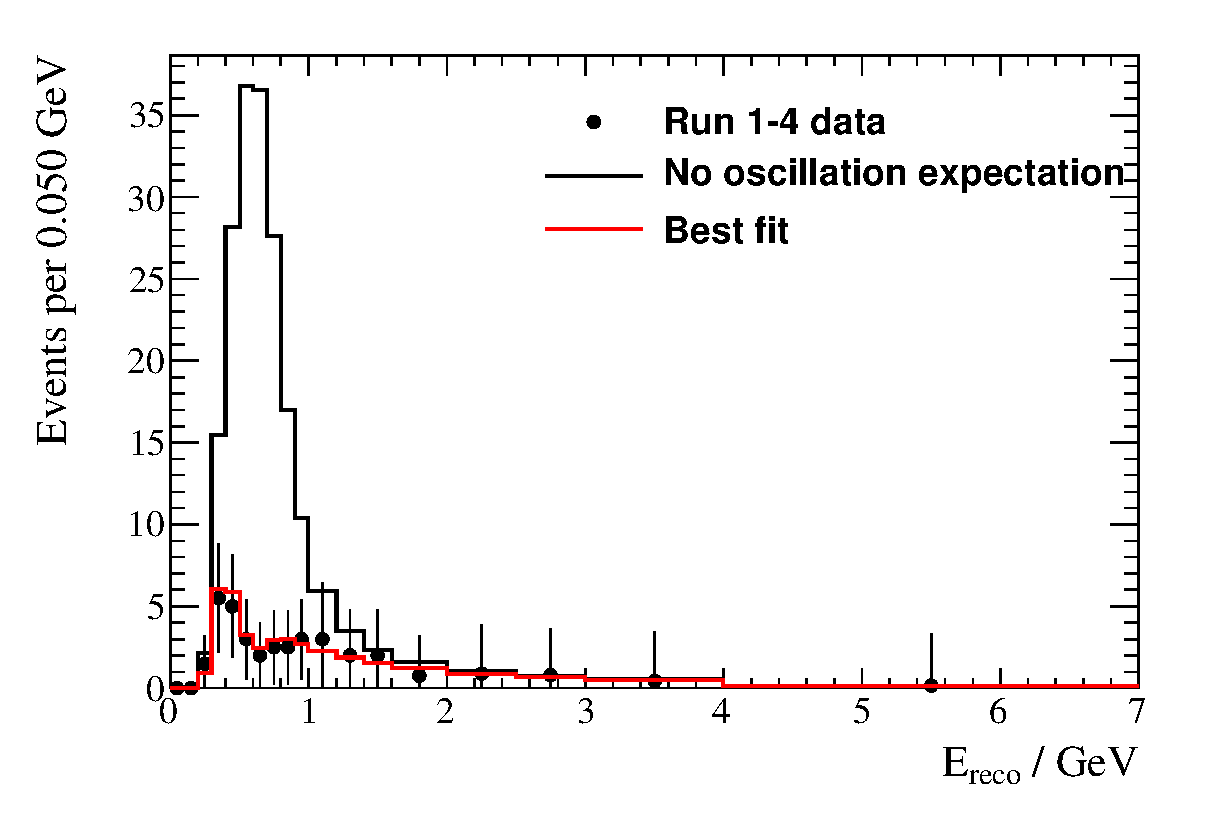
\includegraphics[width=28pc]{./images/data_fit/normal/run1-4_nuis4_sintheta_normal_spectrumper50_rebin}
    \end{minipage}
    \vfill
    \begin{minipage}[t]{0.8\linewidth}
      \center
      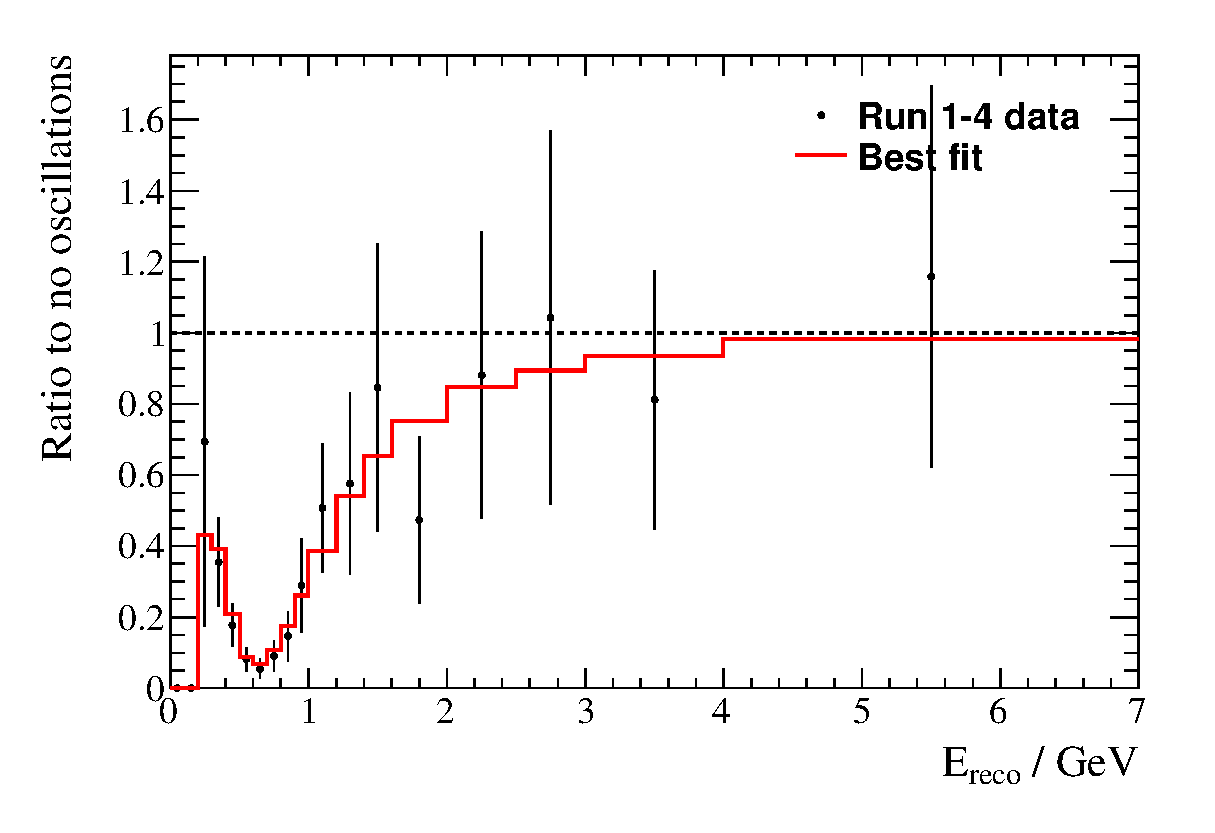
\includegraphics[width=28pc]{./images/data_fit/normal/run1-4_nuis4_sintheta_normal_spectrum_ratio_rebin}
    \end{minipage}
    \caption {
      Best-fit reconstructed energy spectrum (top) obtained from the fit of the combined Run 1+2+3+4 dataset.
      The Run 1+2+3+4 data and the prediction obtained using the no-oscillation hypothesis are also shown.
      The spectra are shown using the coarse binning scheme described in Sec.\ \ref{sec:results_bestfit_spectra}.
      The characteristic energy-dependent deficit can be clearly seen.
      The normal mass hierarchy is assumed.
      \label{fig:results_data1234_spectrum_coarse:normal}
    }
  }
\end{figure*}

\begin{figure*}[htb]
  \centering{
    \begin{minipage}[t]{0.8\linewidth}
      \center
      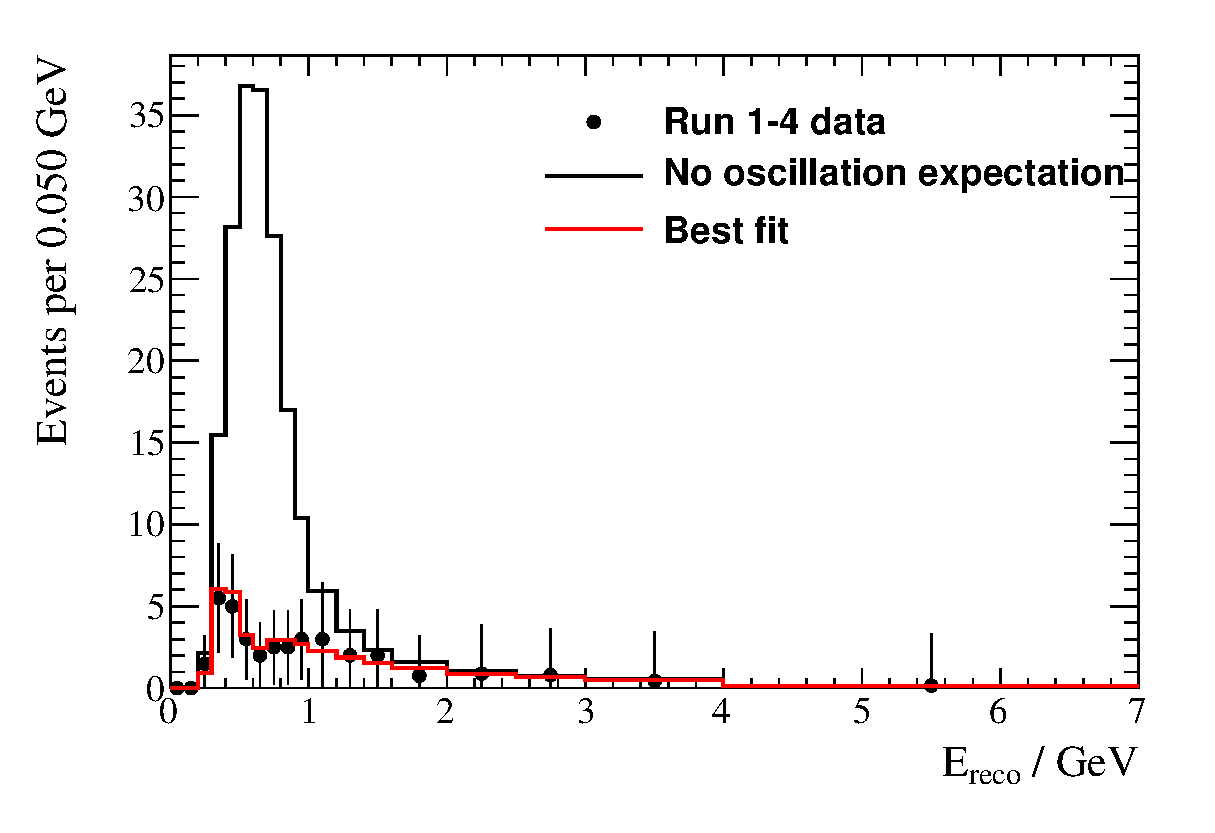
\includegraphics[width=28pc]{./images/data_fit/inverted31/run1-4_nuis4_sintheta_inverted31_spectrumper50_rebin}
    \end{minipage}
    \vfill
    \begin{minipage}[t]{0.8\linewidth}
      \center
      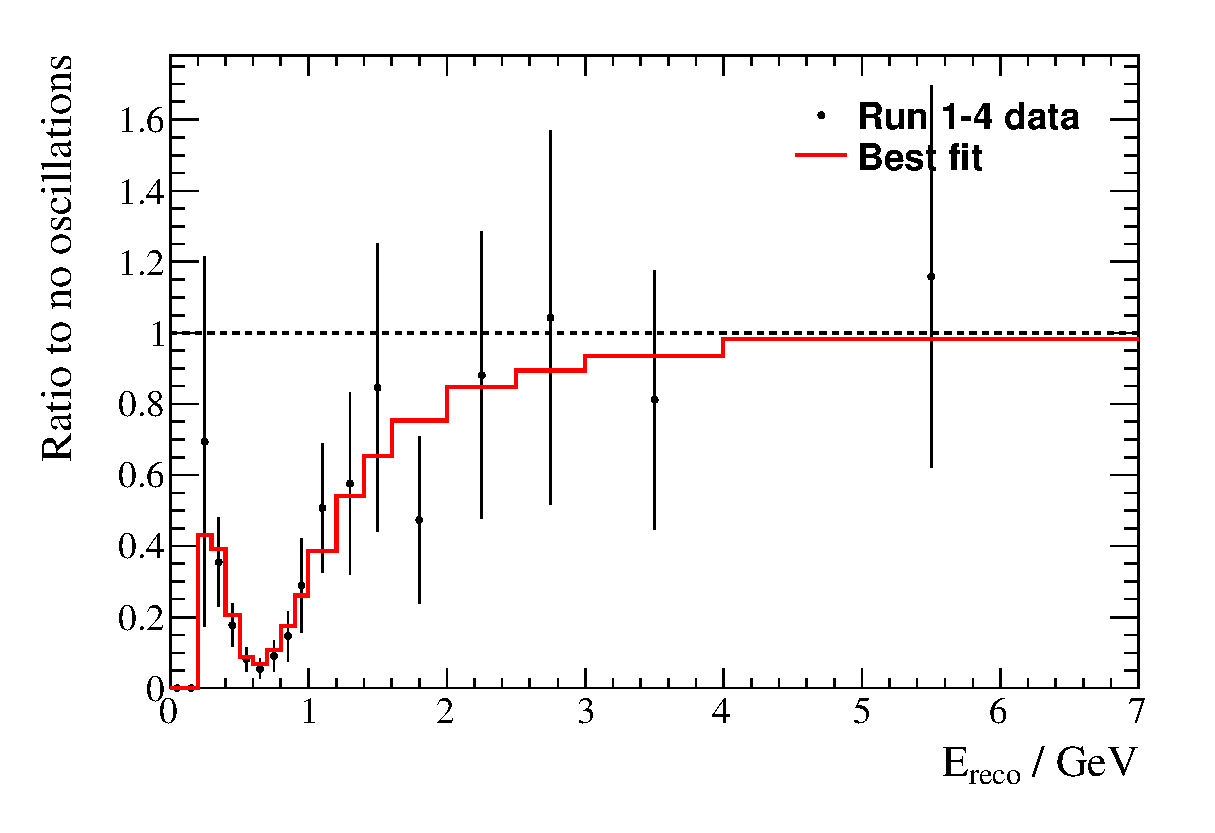
\includegraphics[width=28pc]{./images/data_fit/inverted31/run1-4_nuis4_sintheta_inverted31_spectrum_ratio_rebin}
    \end{minipage}
    \caption {
      Best-fit reconstructed energy spectrum (top) obtained from the fit of the combined Run 1+2+3+4 dataset.
      The Run 1+2+3+4 data and the prediction obtained using the no-oscillation hypothesis are also shown.
      The spectra are shown using the coarse binning scheme described in Sec.\ \ref{sec:results_bestfit_spectra}.
      The characteristic energy-dependent deficit can be clearly seen.
      The inverted mass hierarchy is assumed.
      \label{fig:results_data1234_spectrum_coarse:inverted}
    }
  }
\end{figure*}

\begin{figure*}[htb]
  \begin{minipage}[t]{0.48\linewidth}
    \center
    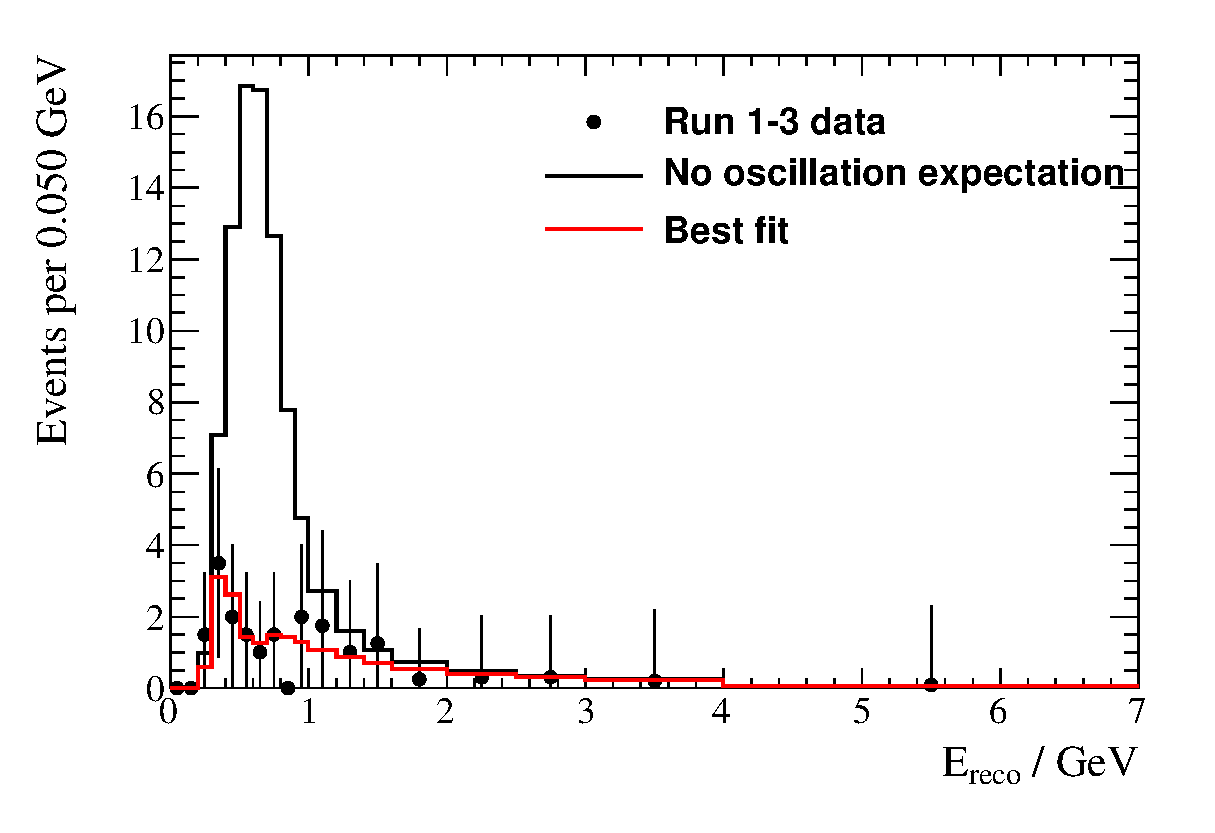
\includegraphics[width=20pc]{./images/data_fit/run123/run1-4_nuis4_sintheta_normal_run123_spectrumper50_rebin}
  \end{minipage}
  \hspace{0.06\linewidth}
  \begin{minipage}[t]{0.48\linewidth}
    \center
    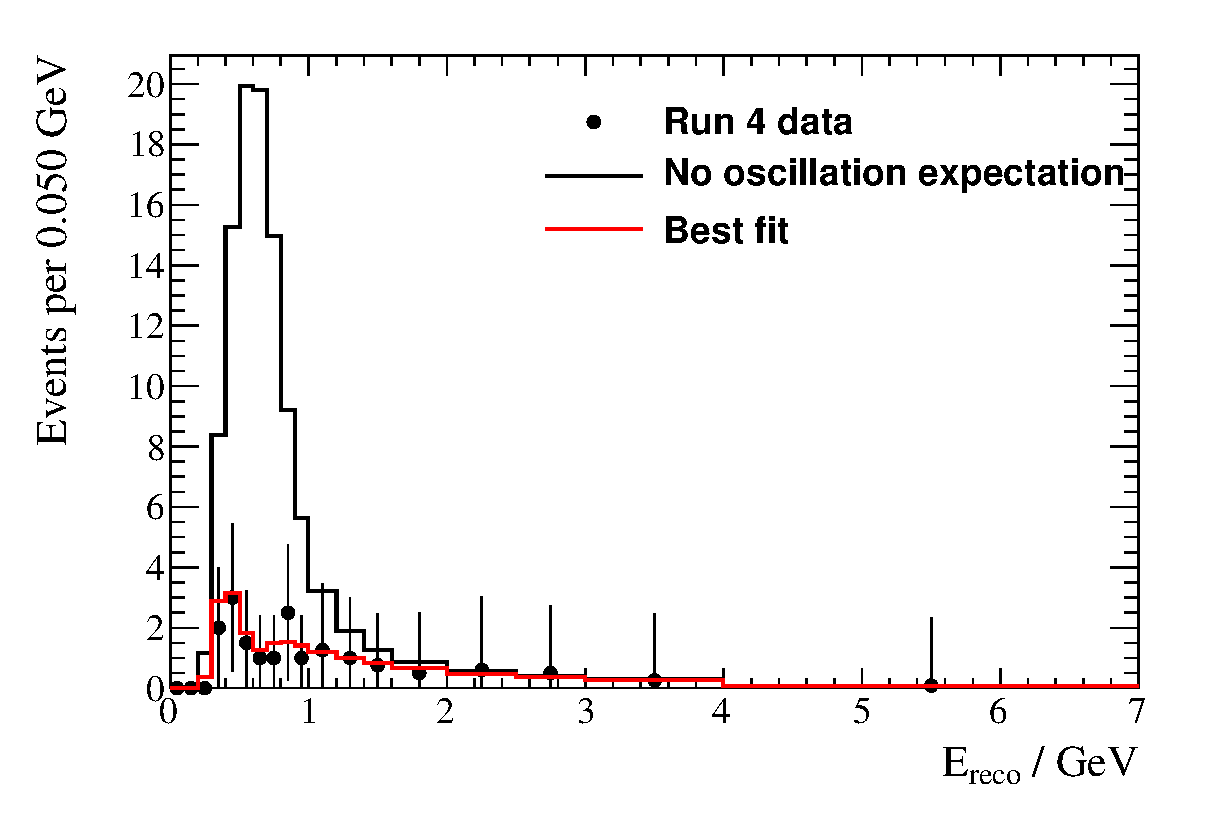
\includegraphics[width=20pc]{./images/data_fit/run4/run1-4_nuis4_sintheta_normal_run4_spectrumper50_rebin}
  \end{minipage}
  \vfill
  \begin{minipage}[t]{0.48\linewidth}
    \center
    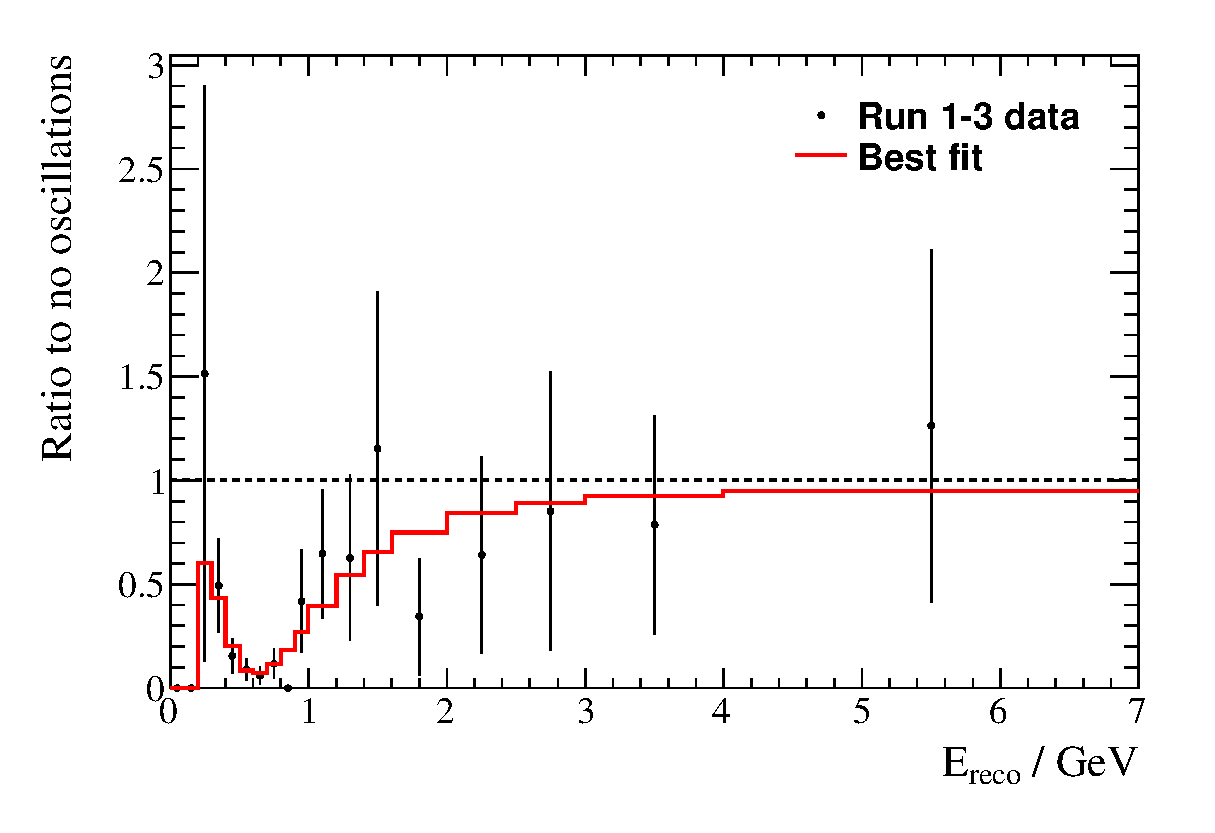
\includegraphics[width=20pc]{./images/data_fit/run123/run1-4_nuis4_sintheta_normal_run123_spectrum_ratio_rebin}
    \caption {
      Best-fit reconstructed energy spectrum (top) obtained from the fit of the combined Run 1+2+3 dataset only.
      The Run 1+2+3 data and the prediction obtained using the no-oscillation hypothesis are also shown.
      The spectra are shown using the coarse binning scheme described in Sec.\ \ref{sec:results_bestfit_spectra}.
      The characteristic energy-dependent deficit can be clearly seen.
      The normal mass hierarchy is assumed.
    }
    \label{fig:results_data123_spectrum_coarse}
  \end{minipage}
  \hspace{0.06\linewidth}
  \begin{minipage}[t]{0.48\linewidth}
    \center
    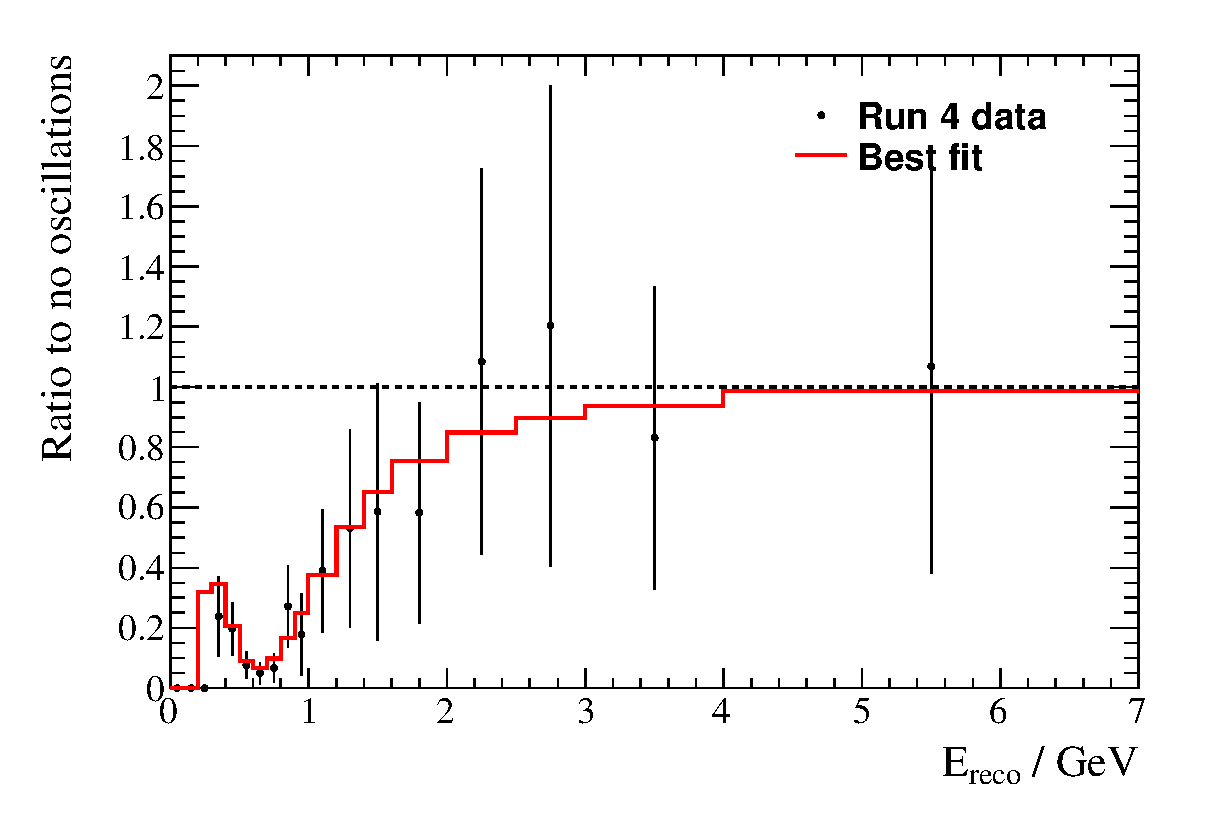
\includegraphics[width=20pc]{./images/data_fit/run4/run1-4_nuis4_sintheta_normal_run4_spectrum_ratio_rebin}
    \caption {
      Best-fit reconstructed energy spectrum (top) obtained from the fit of the combined Run 4 dataset only.
      The Run 4 data and the prediction obtained using the no-oscillation hypothesis are also shown.
      The spectra are shown using the coarse binning scheme described in Sec.\ \ref{sec:results_bestfit_spectra}.
      The characteristic energy-dependent deficit can be clearly seen.
      The normal mass hierarchy is assumed.
    }
    \label{fig:results_data4_spectrum_coarse}
  \end{minipage}
\end{figure*}


%...........................................................
%
% Best-fit spectra (total and components) for `2+N' fit 
% (Run1+2+3+4 only, 73 bins)
%

\begin{figure*}[htb]
  \center
  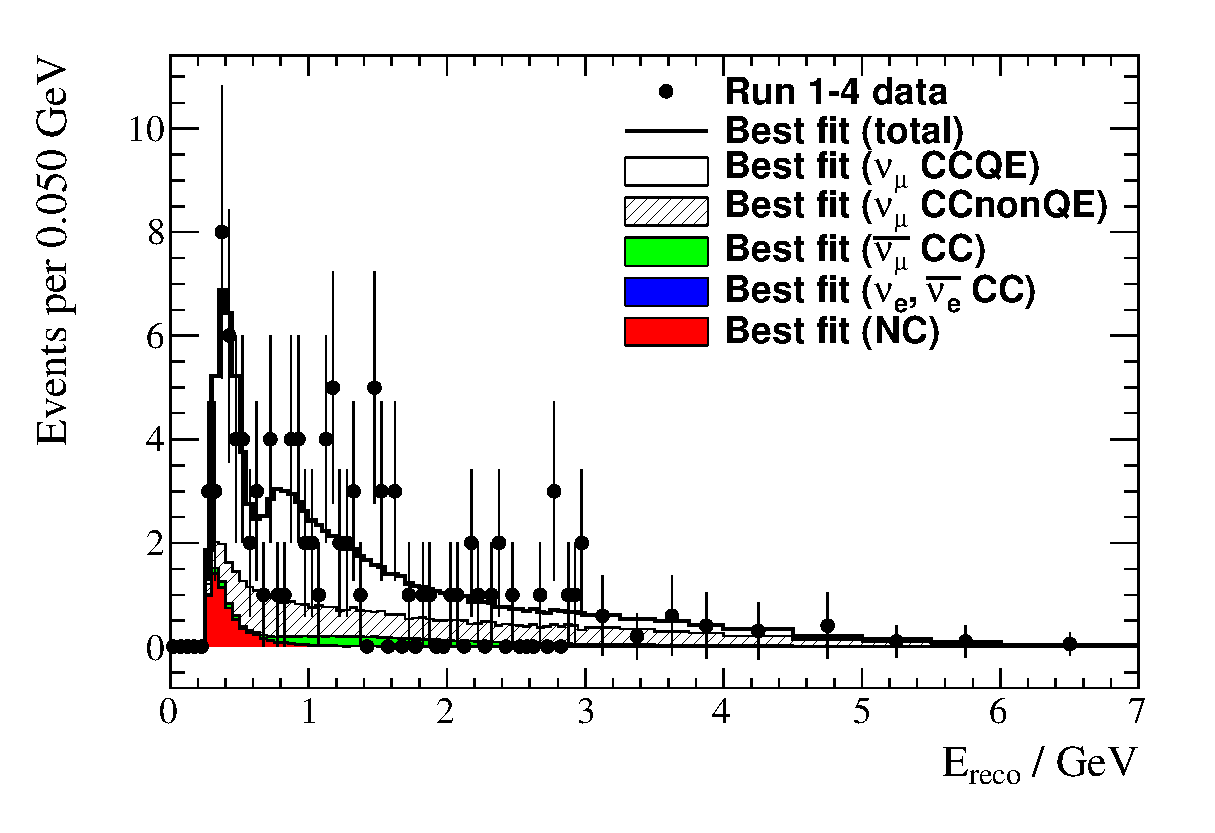
\includegraphics[width=28pc]{./images/data_fit/normal/run1-4_nuis4_sintheta_normal_spectrumper50_components}
  \caption {
    Best-fit reconstructed energy spectrum in the 73-bin scheme used in the fit (see Sec.\ref{sec:mc_templates:template_binning})
    and its components
    obtained from the fit of the Run 1+2+3+4 dataset.  
    The 32 components, each of which is calculated separately in the analysis, are grouped into just 5 categories:
    $\nu_{\mu}$ CCQE, $\nu_{\mu}$ CCnQE, $\bar{\nu_{\mu}}$ CC, $\nu_{e}$/$\bar{\nu_{e}}$ CC and NC.  
    The normal mass hierarchy is assumed.
  }
  \label{fig:results_data1234_spectrum_components:normal}
\end{figure*}

\begin{figure*}[htb]
  \center
  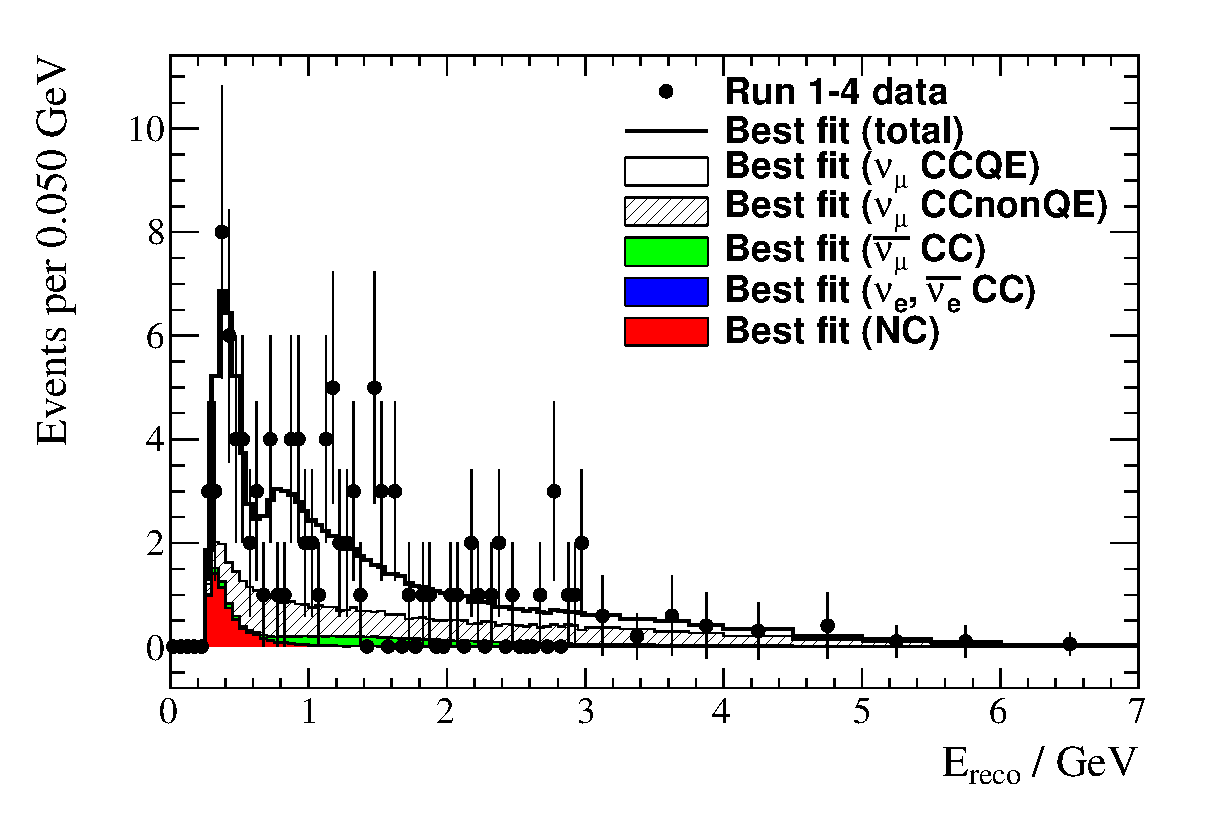
\includegraphics[width=28pc]{./images/data_fit/inverted31/run1-4_nuis4_sintheta_inverted31_spectrumper50_components}
  \caption {
    Best-fit reconstructed energy spectrum in the 73-bin scheme used in the fit (see Sec.\ \ref{sec:mc_templates:template_binning}))
    and its components
    obtained from the fit of the Run 1+2+3+4 dataset.  
    The 32 components, each of which is calculated separately in the analysis, are grouped into just 5 categories:
    $\nu_{\mu}$ CCQE, $\nu_{\mu}$ CCnQE, $\bar{\nu_{\mu}}$ CC, $\nu_{e}$/$\bar{\nu_{e}}$ CC and NC.  
    The inverted mass hierarchy is assumed.
  }
  \label{fig:results_data1234_spectrum_components:inverted}
\end{figure*}


%...........................................................
%
% Best-fit spectra comparisons between normal & inverted hierarchy (73 bin and coarse binning)
%
\begin{figure*}[htb]
\center
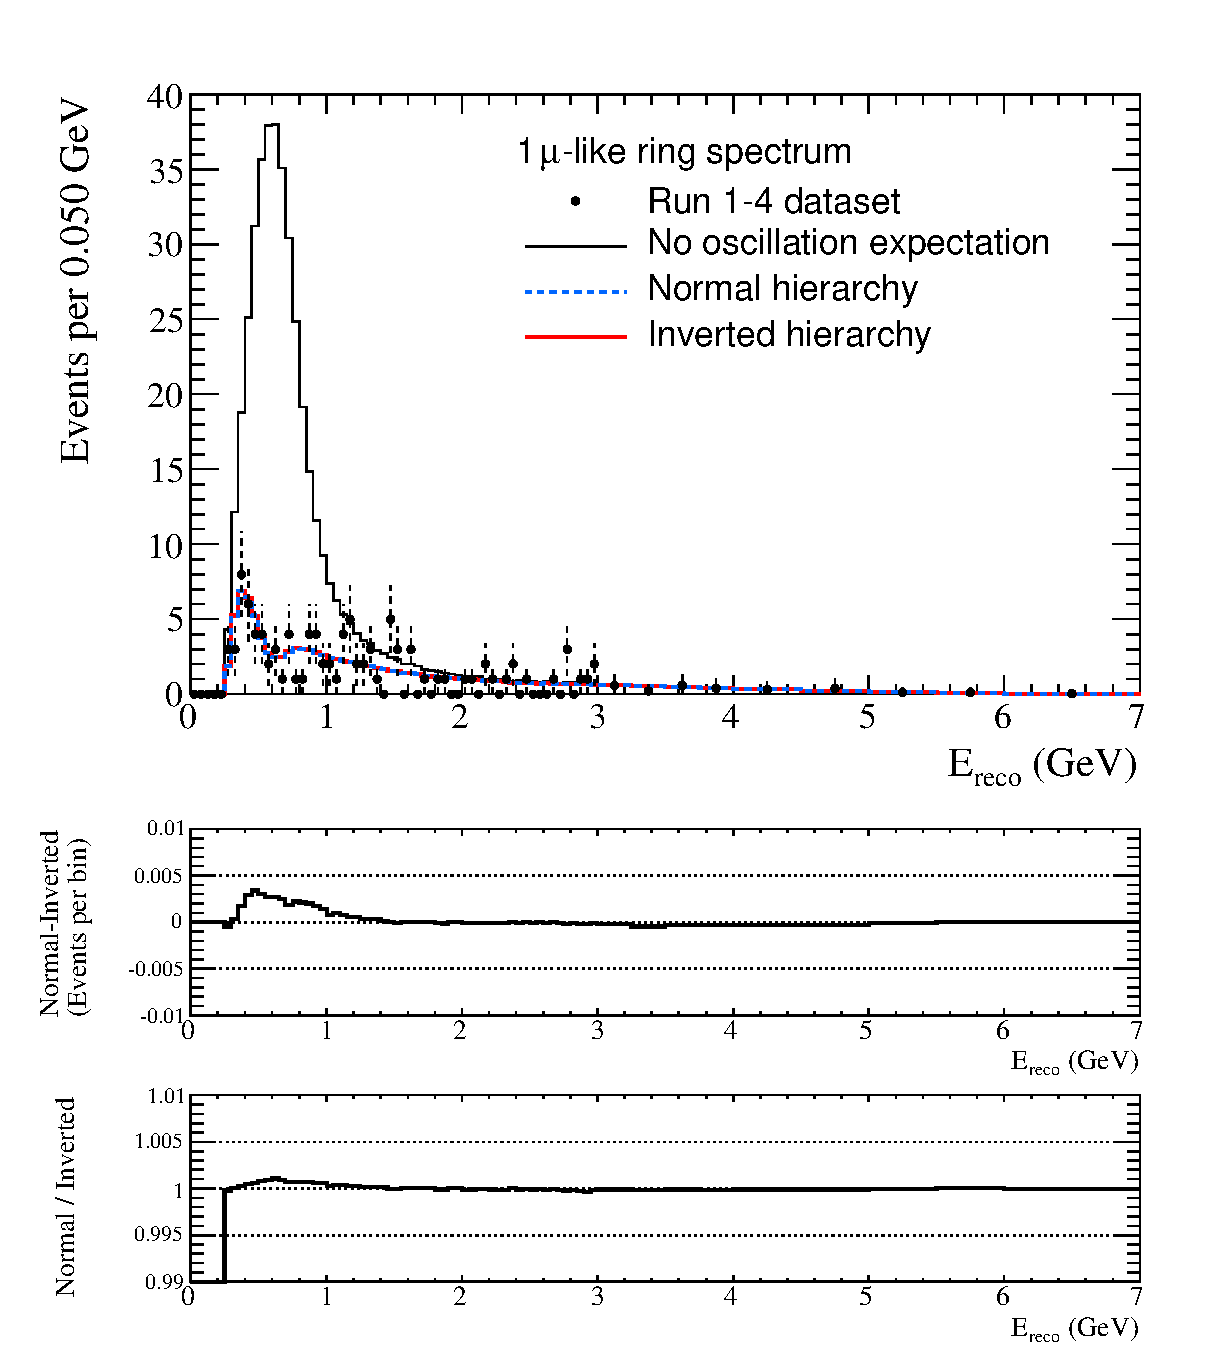
\includegraphics[width=40pc]{./images/data_fit/compare/spectrum_comparison_normal_inverted}
\caption {
  Comparison between best-fit reconstructed energy spectra
  obtained from the normal and inverted mass hierarchy fits of the Run 1+2+3+4 dataset.
  The spectra are shown using the 73 bins used in the fit (see Sec.\ \ref{sec:mc_templates:template_binning}).
  Also shown are the absolute difference between the normal and inverted mass hierarchy
  best-fit predicted spectra and the ratio between them.
}
\label{fig:results_data1234_spectrum_comparison}
\end{figure*}

\begin{figure*}[htb]
\center
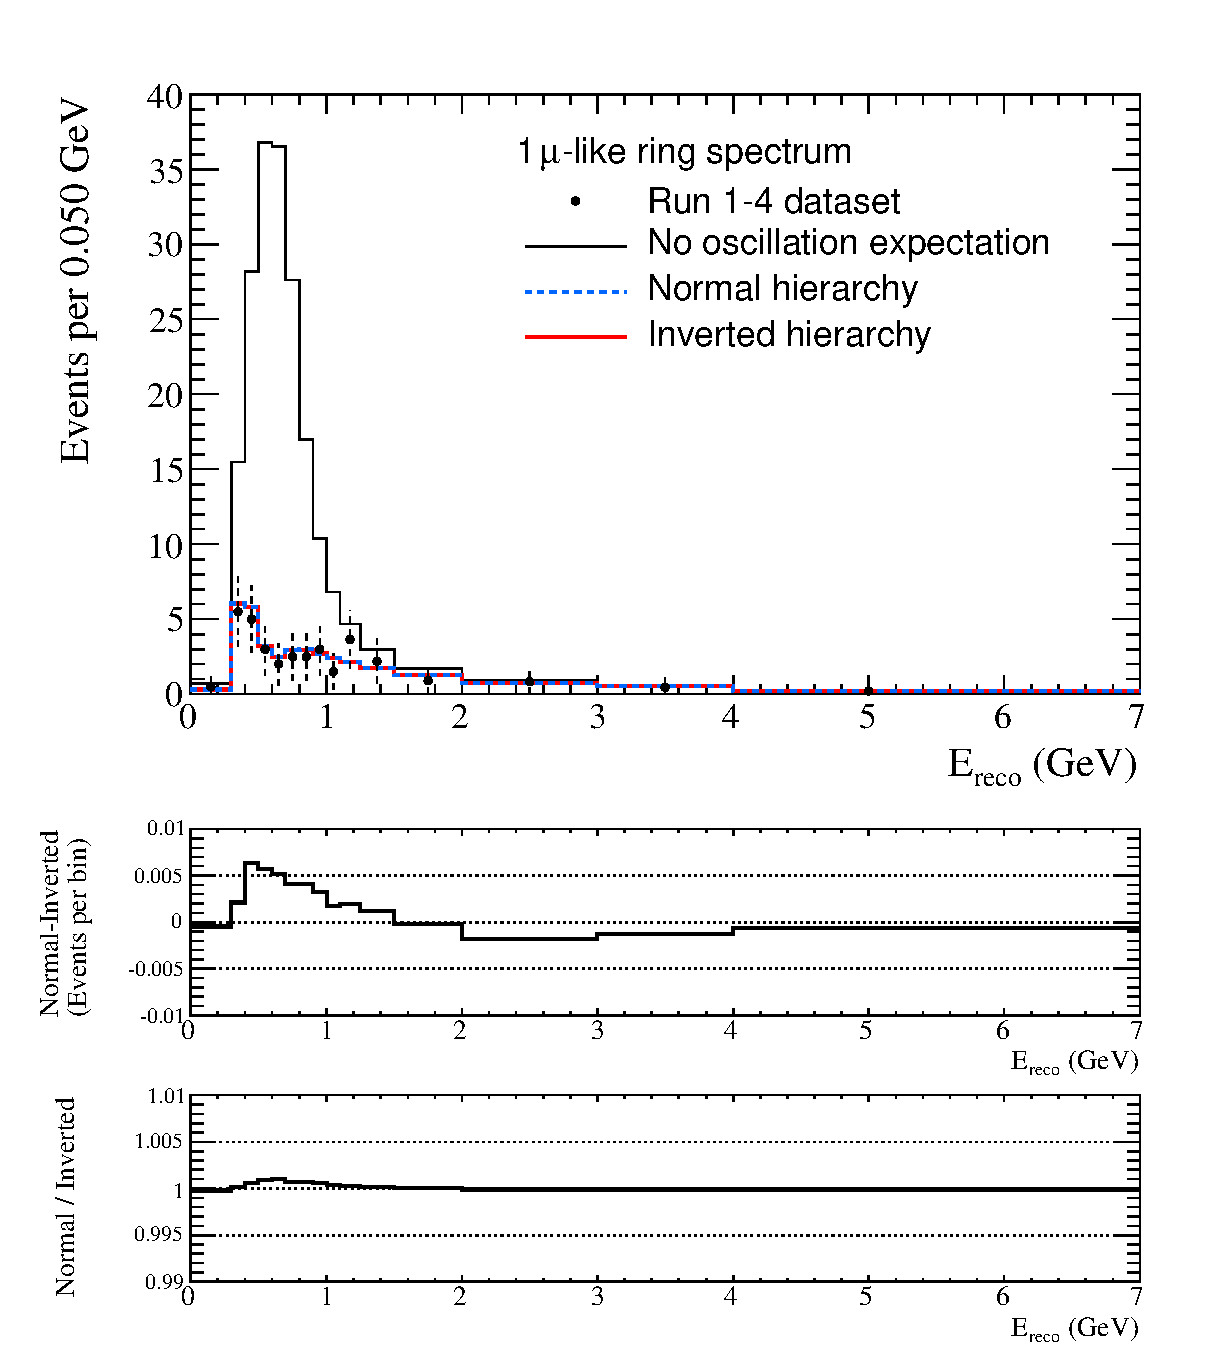
\includegraphics[width=40pc]{./images/data_fit/compare/spectrum_comparison_normal_inverted_coarse}
\caption {
  Comparison between best-fit reconstructed energy spectra
  obtained from the normal and inverted mass hierarchy fits of the Run 1+2+3+4 dataset.
  The spectra are shown using the coarse binning scheme described in Sec.\ \ref{sec:results_bestfit_spectra}.
  Also shown are the absolute difference between the normal and inverted mass hierarchy
  best-fit spectra and the ratio between them.
}
\label{fig:results_data1234_spectrum_comparison_coarse}
\end{figure*}



%...........................................................
%
% Best-fit spectra comparisons between normal run 1+2+3, 4, 1+2+3+4 (73 bin and coarse binning)
%
\begin{figure*}[htb]
\center
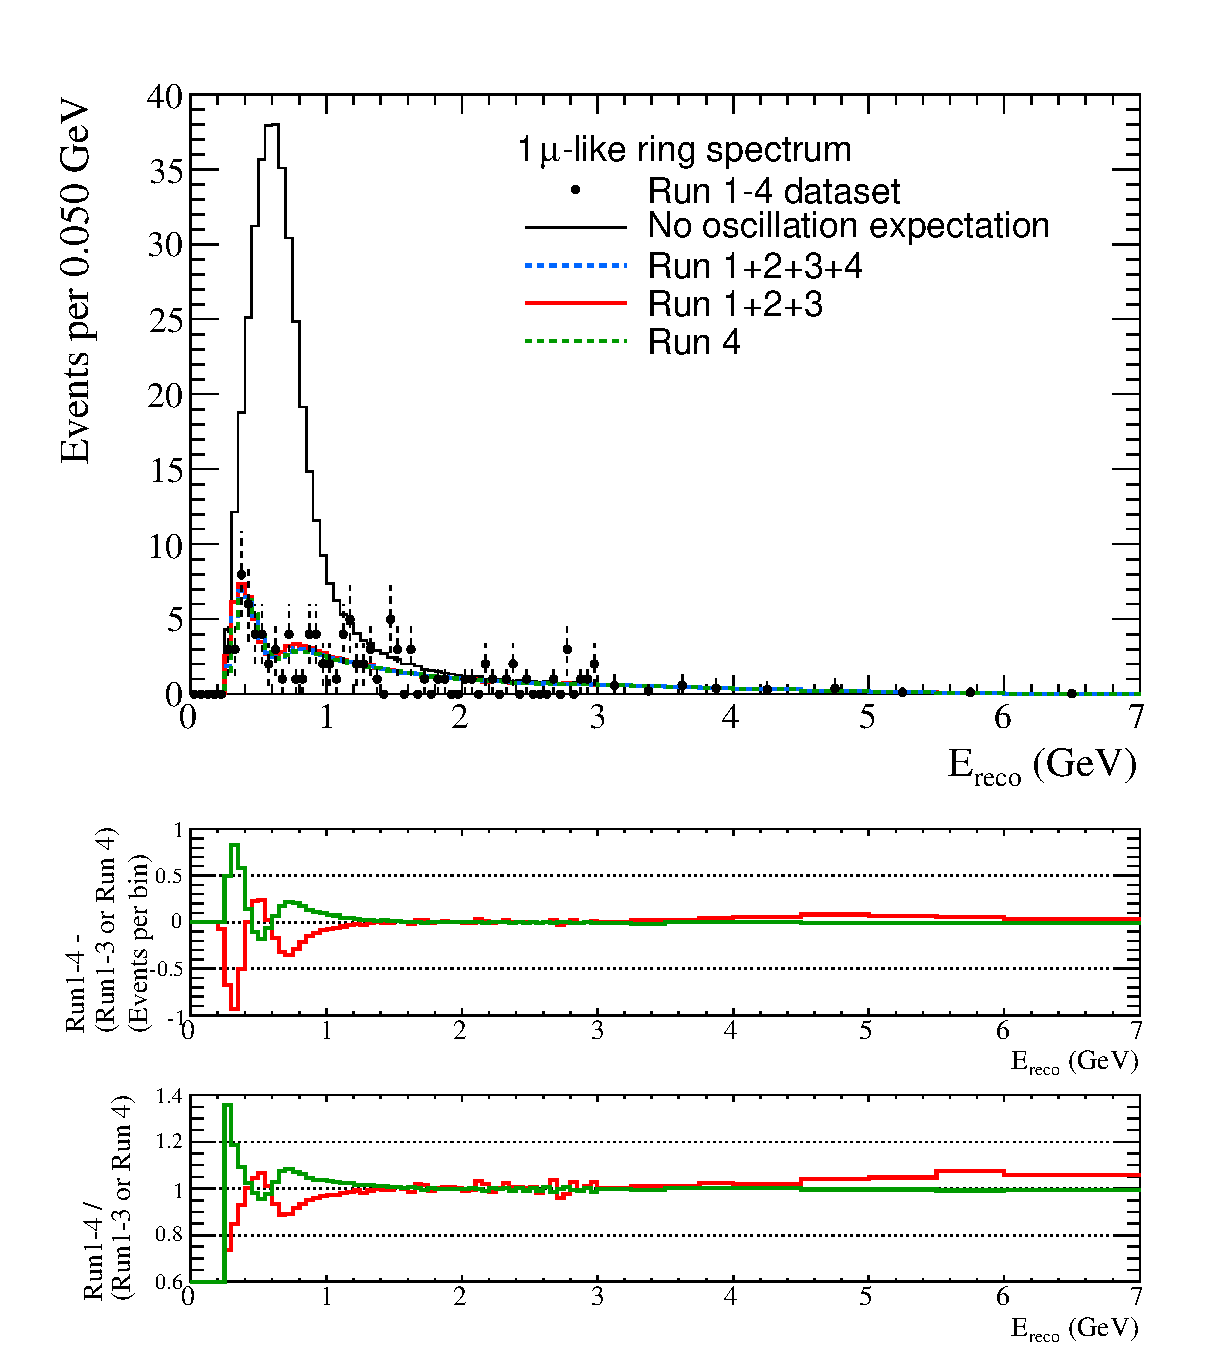
\includegraphics[width=40pc]{./images/data_fit/compare/spectrum_comparison_sepruns}
\caption {
  Comparison between best-fit reconstructed energy spectra
  obtained from the fits to the Run 1+2+3, Run 4, and Run 1+2+3+4 datasets, all scaled to the Run 1+2+3+4 POT,
  for the normal mass hierarchy.
  The spectra are shown using the 73 bins used in the fit (see Sec.\ \ref{sec:mc_templates:template_binning}).
  Also shown are the absolute difference between the scaled Run 1+2+3 or Run 4 best-fit predicted spectra and 
  the Run 1+2+3+4 spectrum and the ratio between them.
}
\label{fig:results_dataruns_spectrum_comparison}
\end{figure*}

\begin{figure*}[htb]
\center
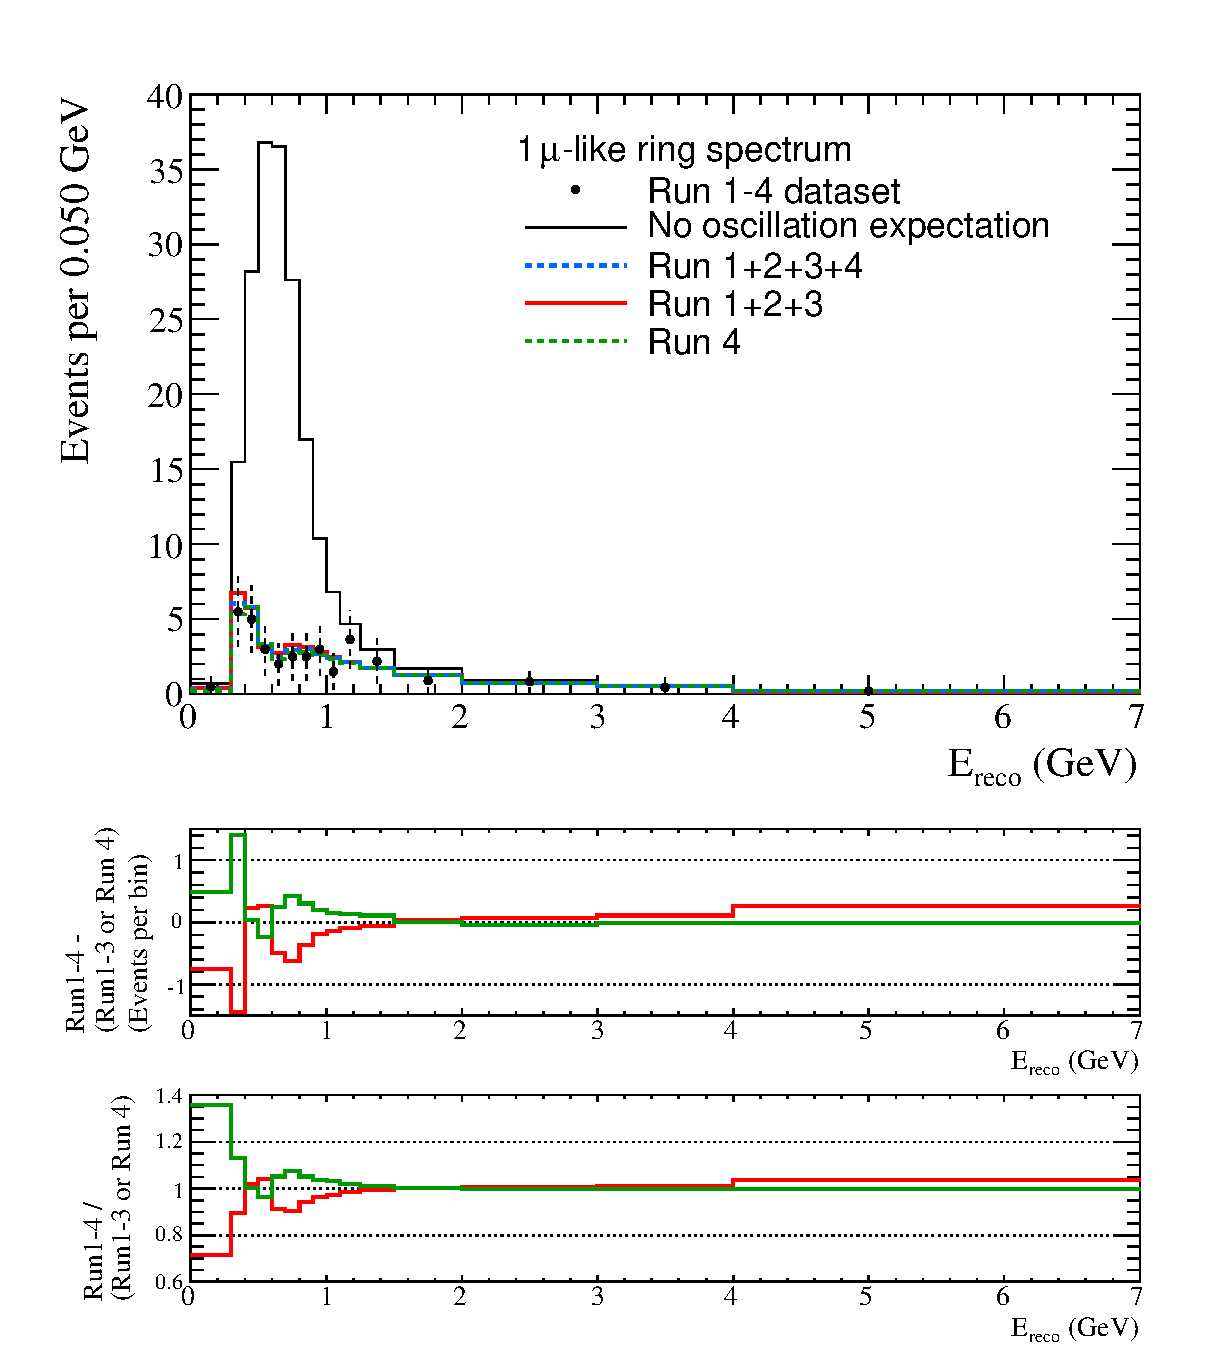
\includegraphics[width=40pc]{./images/data_fit/compare/spectrum_comparison_sepruns_coarse}
\caption {
  Comparison between best-fit reconstructed energy spectra
  obtained from the fits to the Run 1+2+3, Run 4, and Run 1+2+3+4 datasets, all scaled to the Run 1+2+3+4 POT,
  for the normal mass hierarchy.
  The spectra are shown using the coarse binning scheme described in Sec.\ \ref{sec:results_bestfit_spectra}.
  Also shown are the absolute difference between the scaled Run 1+2+3 or Run 4 best-fit predicted spectra and 
  the Run 1+2+3+4 spectrum and the ratio between them.
}
\label{fig:results_dataruns_spectrum_comparison_coarse}
\end{figure*}

%--------------------------------------------------------------------------------------
% Contours
%--------------------------------------------------------------------------------------

\clearpage

\subsection {Confidence regions}
\label{sec:results_contours}

The first step in constructing confidence contours in the 2-dimensional $\sin^{2}\theta_{23}$ - $|\Delta m^{2}_{32}|$ or 
$\sin^{2}\theta_{23}$ - $|\Delta m^{2}_{31}|$
oscillation parameter space is to construct the $\Delta\chi^2$ surface from the fit of the data.
The oscillation parameter space is divided into a rectangular grid of width $\sin^{2}\theta_{23}$ = 0.0025, $|\Delta m^{2}_{32}|$ 
or $|\Delta m^{2}_{31}|$ = 0.025$\times$10$^{-3}$ eV$^{2}$/c$^{4}$, with a grid point at the centre of each rectangle. For each 
mass hierarchy, two separate fits are made of 
the data at each grid point: in one fit, the values of $\sin^{2}\theta_{23}$ and $|\Delta m^{2}_{32}|$ or $|\Delta m^{2}_{31}|$ 
are fixed to the true values of the grid point and the 41 systematic and four non-23 oscillation parameters are allowed to float, 
while, in the other fit, $\sin^{2}\theta_{23}$, $|\Delta m^{2}_{32}|$ or $|\Delta m^{2}_{31}|$,  and the systematic and non-23 
oscillation parameters are allowed to float. $\Delta\chi^2$ is then calculated as the 
difference between the minimum values of $\chi^{2}$ from the two fits ($\chi^{2}$ is defined in Eq.\
\ref{eq:chisquare} in Sec.\ \ref{sec:oscfit_method}).

These 2-dimensional $\Delta\chi^2$ surfaces from the fits of the Run 1+2+3+4 dataset are shown in
Figs.\ \ref{fig:results_data1234_chisq:normal} and \ref{fig:results_data1234_chisq:inverted}
as a function of $\sin^{2}\theta_{23}$ and $|\Delta m^{2}_{32}|$ or $|\Delta m^{2}_{31}|$,
for the normal and inverted mass hierarchies respectively.
For comparison, the corresponding $\Delta\chi^2$ surfaces from the fits of the Run 1+2+3 and Run 4
datasets are shown for the normal mass hierarchy 
in Figs.\ \ref{fig:results_data123_chisq} and \ref{fig:results_data4_chisq} respectively.
The same $\Delta\chi^2$ range is used in all colour plots to allow comparison.

Confidence regions were constructed in the 2-dimensional parameter space $\sin^{2}\theta_{23}$ and $|\Delta m^{2}_{32}|$ or $|\Delta m^{2}_{31}|$
using the constant-$\Delta\chi^2$ method described in Sec.\ \ref{sec:contour_construction} from the
fits of the Run 1+2+3+4, Run 1+2+3 and Run 4 datasets.
The 68\% and 90\% CL regions are shown
in Figs.\ \ref{fig:results_data1234_contour:normal} and \ref{fig:results_data1234_contour:inverted}
for the normal and inverted mass hierarchies respectively.
The corresponding constant-$\Delta\chi^2$ contours for the Run 1+2+3 and Run 4 datasets are shown
in Figs.\ \ref{fig:results_data123_contour} and \ref{fig:results_data4_contour} respectively.

To construct 2-dimensional confidence regions using the method of Feldman and Cousins \cite{FeldmanCousins},
the $\Delta\chi^{2}_{critical}$ surfaces must be calculated in the $\sin^{2}\theta_{23}$ - $|\Delta m^{2}_{32}|$
or $\sin^{2}\theta_{23}$ - $|\Delta m^{2}_{31}|$ oscillation parameter space as described in Sec.\ \ref{sec:contour_construction}.
In Figs.\ \ref{fig:fc_dchisqcrit_2d:normal} and \ref{fig:fc_dchisqcrit_2d:inverted}, we show a Monte Carlo estimation
of the 2-dimensional Feldman-Cousins $\Delta\chi^{2}_{critical}$ values
used for calculation of the 68\% and 90\% CL confidence regions for the normal mass hierarchy and inverted mass hierarchy respectively.
These $\Delta\chi^{2}_{critical}$ surfaces were generated using an ensemble of toy MC experiments which included both
randomized systematic variations and statistical fluctuations.
One-dimensional slices of these $\Delta\chi^{2}_{critical}$ surfaces
are shown in Figs.\ \ref{fig:fc_dchisqcrit_slice_mixing:normal} and \ref{fig:fc_dchisqcrit_slice_dmsq:normal} for the normal mass hierarchy,
and in Figs.\ \ref{fig:fc_dchisqcrit_slice_mixing:inverted} and \ref{fig:fc_dchisqcrit_slice_dmsq:inverted} for the inverted mass hierarchy.
The Feldman-Cousins values of $\Delta\chi^{2}_{critical}$ are lower than the canonical constant-$\Delta\chi^{2}_{critical}$ values
when the true input value of $\sin^2 \theta_{23}$ is near the value of maximal $\nu_{\mu}$ disappearance. 
Under these circumstances, the best-fit values of $\sin^2 \theta_{23}$ pile up at the value of maximal disappearance, and this gives lower
values of $\Delta\chi^{2}$ than would be obtained if that boundary did not exist. Consequently, the 68\% and 90\% critical $\Delta\chi^{2}$
values are lower than the canonical constant-$\Delta\chi^{2}$ values.

Using the $\Delta\chi^2$ and $\Delta\chi^{2}_{critical}$ surfaces presented here,
the 2-dimensional Feldman-Cousins 68\% and 90\% CL regions were constructed
and they are shown in Figs.\ \ref{fig:results_data1234_fc_contour:normal} and
\ref{fig:results_data1234_fc_contour:inverted}.

Profile $\Delta\chi^2$ distributions were also calculated from the 2-dimensional $\Delta\chi^2$ surfaces, and are shown as a 
function of $\sin^{2}\theta_{23}$ and $|\Delta m^{2}_{32}|$ or $|\Delta m^{2}_{31}|$ from the
fits of the Run 1+2+3+4 dataset in 
Figs.\ \ref{fig:results_marg_dchisq_dmsq_normalinverted} and \ref{fig:results_marg_dchisq_sinsq_normalinverted} respectively.
These profile $\Delta\chi^2$ distributions are compared with those from the fits of the Run 1+2+3 and Run 4 datasets for the normal 
mass hierarchy in Figs.\ \ref{fig:results_marg_dchisq_dmsq_all3} and \ref{fig:results_marg_dchisq_sinsq_all3}
for $\sin^{2}\theta_{23}$ and $|\Delta m^{2}_{32}|$ respectively.
Using these plots and the constant-$\Delta\chi^2$ method described in Sec.\ \ref{sec:contour_construction},
1-dimensional limits on the parameters can be obtained for each parameter separately\footnote{
For 1 fit parameter, the critical values of $\Delta{\chi^{2}}$ used are 
1.00 (68\% CL), 2.71 (90\% CL), 3.84 (95\% CL), 6.63 (99\% CL).
For 2 parameters fitted simultaneously, the critical values of $\Delta{\chi^{2}}$ used are 
2.30 (68\% CL), 4.61 (90\% CL), 5.99 (95\% CL), 9.21 (99\% CL).
}.
These limits are presented in Tab.\ \ref{tab:data_fits:1dlimits}.

1-dimensional confidence intervals were also constructed separately for each of $\sin^2 \theta_{23}$ and $|\Delta m_{32}^{2}|$ (normal mass hierarchy) 
or $|\Delta m_{31}^{2}|$ (inverted mass hierarchy) using the new procedure described in Sec.\ \ref{sec:contour_construction}. For the normal 
mass hierarchy, a Monte Carlo estimation of the 68\% and 90\% 1D critical $\Delta\chi^{2}$ values for $\sin^2 \theta_{23}$ was made using 
10000 toy experiments with systematic variations and statistical fluctuations at each value of that parameter, with the input values of 
$|\Delta m_{32}^{2}|$ being chosen using the method described in Sec.\ \ref{sec:contour_construction}. These critical $\Delta\chi^{2}$ values are shown in 
Fig.\ \ref{fig:results_1D_dchisq_sinsq_normal}, in which they are fitted with cubic splines. The 68\% and 90\% confidence intervals in 
$\sin^2 \theta_{23}$ include the values of that parameter for which $\Delta\chi^{2}$ from the 1D fit of the Run 1+2+3+4 data is less than the 
appropriate MC critical values. In practice, this was done by finding the values of $\sin^2 \theta_{23}$ where the cubic splines intersect the 
plot of the 1D $\Delta\chi^{2}$ from the fit of the data (see Fig.\ \ref{fig:results_1D_dchisq_sinsq_normal}). The 68\% and 90\% confidence 
intervals in $|\Delta m_{32}^{2}|$ were constructed in a similar way, and the MC critical $\Delta\chi^{2}$ values and the 1D $\Delta\chi^{2}$ 
from the fit of the data are shown in Fig.\ \ref{fig:results_1D_dchisq_dm32sq_normal}. 

In Fig.\ \ref{fig:results_1D_dchisq_sinsq_normal}, it is apparent that the MC critical $\Delta\chi^{2}$ values are lower than the canonical 
constant-$\Delta\chi^{2}$ values when the true input value of $\sin^2 \theta_{23}$ is near the value of maximal $\nu_{\mu}$ disappearance. 
Again this is due to the best-fit values of $\sin^2 \theta_{23}$ in the toy MC experiments piling up at the value of maximal disappearance.
At input values of $\sin^2 \theta_{23}$ far from the value of maximal 
$\nu_{\mu}$ disappearance, the critical $\Delta\chi^{2}$ values approach the canonical constant-$\Delta\chi^{2}$ values as expected. The MC 
critical $\Delta\chi^{2}$ values for $|\Delta m_{32}^{2}|$ are lower than the canonical constant-$\Delta\chi^{2}$ values for all input values 
of that parameter. This is due to the input values of $\sin^2 \theta_{23}$ to the toy experiments, many of which are near the value of maximal 
$\nu_{\mu}$ disappearance (see Fig.\ \ref{fig:input_mixing23_1DFC} for an example). Again the best-fit values of $\sin^2 \theta_{23}$ pile up 
at the value of maximal disappearance, which results in lower values of $\Delta\chi^{2}$ than would occur if that boundary were not present. 

For the inverted mass hierarchy, the Monte Carlo estimations of the 68\% and 90\% 1D critical $\Delta\chi^{2}$ values for $\sin^2 \theta_{23}$ 
were made using input values of $|\Delta m_{31}^{2}|$ that were chosen according to the method described in Sec.\ \ref{sec:contour_construction}. 
These critical $\Delta\chi^{2}$ values are compared with the $\Delta\chi^{2}$ from the 1D fits of the Run 1+2+3+4 data in Figs.\ 
\ref{fig:results_1D_dchisq_sinsq_inverted} and \ref{fig:results_1D_dchisq_dm32sq_inverted}; the results show a similar pattern to those for 
the normal mass hierarchy.

The 68\% and 90\% confidence intervals from the new procedure in $\sin^2 \theta_{23}$ and $|\Delta m_{32}^{2}|$ (normal mass hierarchy) or 
$|\Delta m_{31}^{2}|$ (inverted mass hierarchy) are given in Tab.\ \ref{tab:data_fits:1dlimits}. They clearly show that the confidence 
intervals from the constant-$\Delta\chi^{2}$ method overcover for both $\sin^2 \theta_{23}$ and the mass-squared difference; this overcoverage 
is caused by the boundary effects from the value of maximial disappearance  in $\sin^2 \theta_{23}$.

In the next section, comparisons are presented of the confidence regions obtained 
using different construction methods.
The contours from different running periods are compared, and we also compare our contours
from the fit to the combined Run 1+2+3+4 dataset with recent measurements from MINOS and 
SuperK and T2K 6.5700$\times$10$^{20}$-POT sensitivity contours. 


%...........................................................
%
% \Delta\chisquare surfaces 
%
\begin{figure*}[htb]
  \begin{minipage}[t]{0.96\linewidth}
    \center
    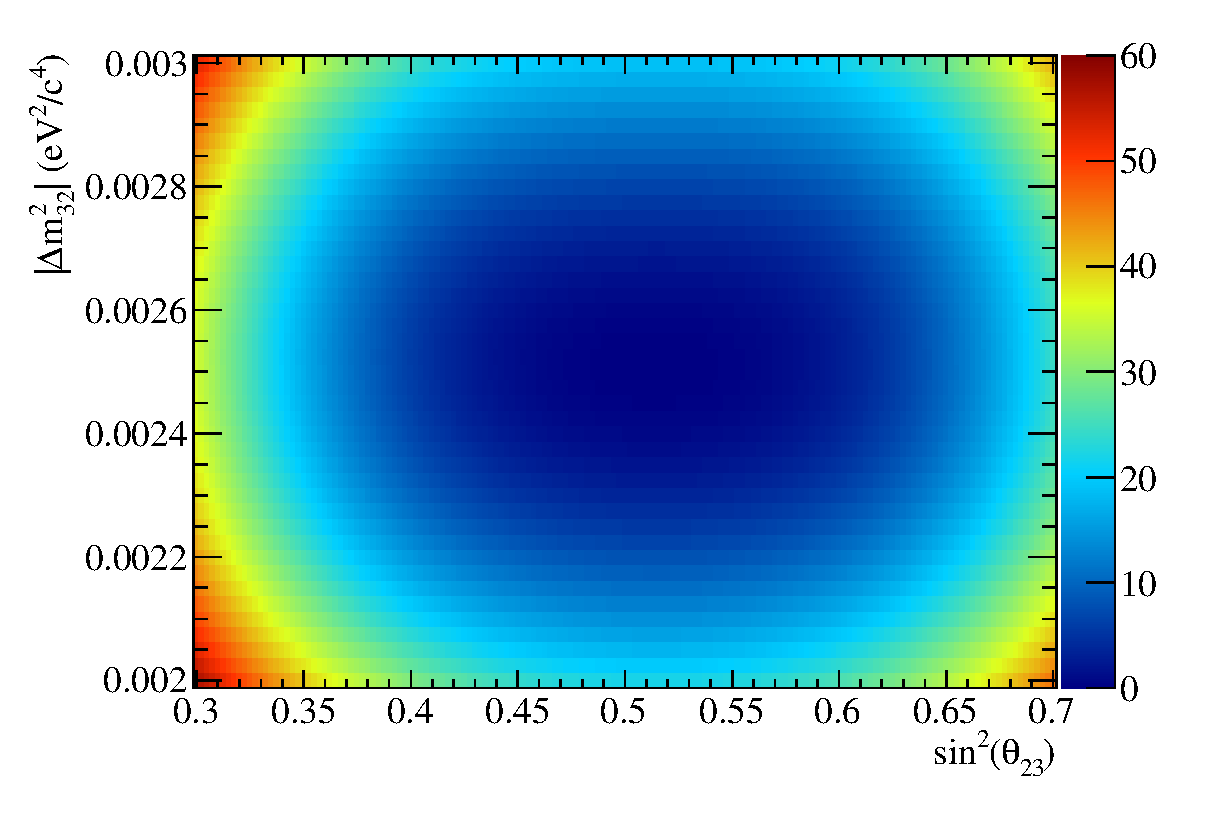
\includegraphics[width=36pc]{./images/data_fit/normal/run1-4_nuis4_sintheta_normal_dchisq_maxz60}
    \caption {
      $\Delta\chi^2$ surface from the fit of the Run 1+2+3+4 dataset.
      The normal mass hierarchy is assumed.
    }
    \label{fig:results_data1234_chisq:normal}
  \end{minipage}
  \vfill
  \begin{minipage}[t]{0.96\linewidth}
    \center
    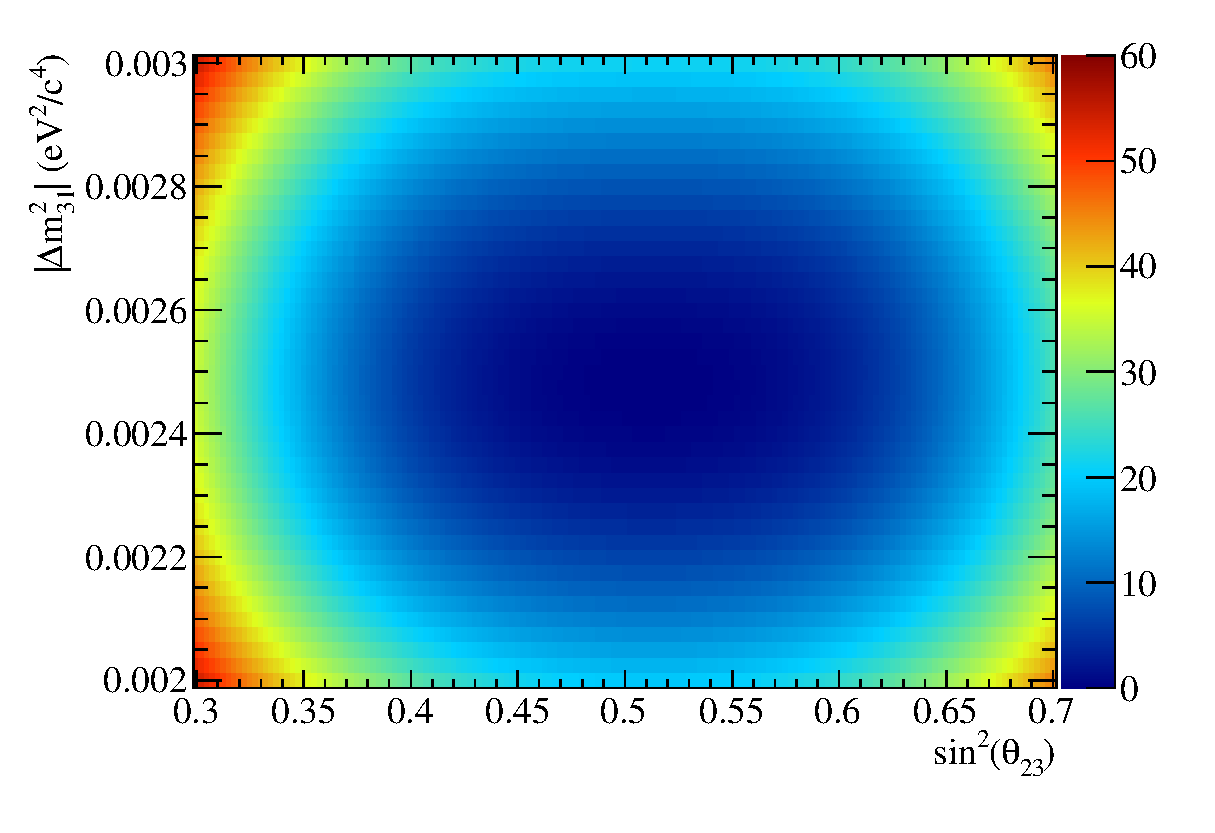
\includegraphics[width=36pc]{./images/data_fit/inverted31/run1-4_nuis4_sintheta_inverted31_dchisq_maxz60}
    \caption {
      $\Delta\chi^2$ surface from the fit of the Run 1+2+3+4 dataset.
      The inverted mass hierarchy is assumed.
    }
    \label{fig:results_data1234_chisq:inverted}
  \end{minipage}
\end{figure*}


\begin{figure*}[htb]
\begin{minipage}[t]{0.48\linewidth}
\center
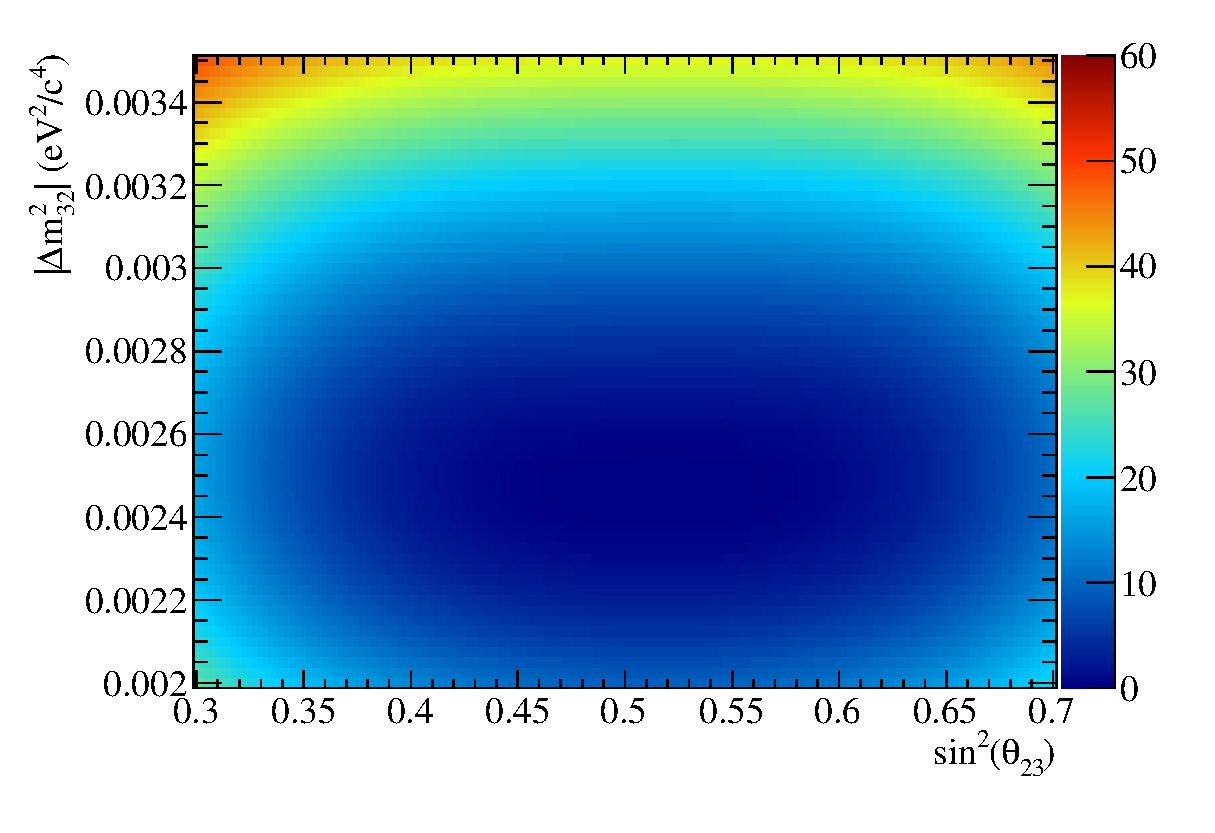
\includegraphics[width=21pc]{./images/data_fit/run123/run1-4_nuis4_sintheta_normal_run123_dchisq_maxz60}
\caption {
  $\Delta\chi^2$ surface from the fit of the Run 1+2+3 dataset.
  The normal mass hierarchy is assumed.
}
\label{fig:results_data123_chisq}
\end{minipage}
\hspace{0.06\linewidth}
\begin{minipage}[t]{0.48\linewidth}
\center
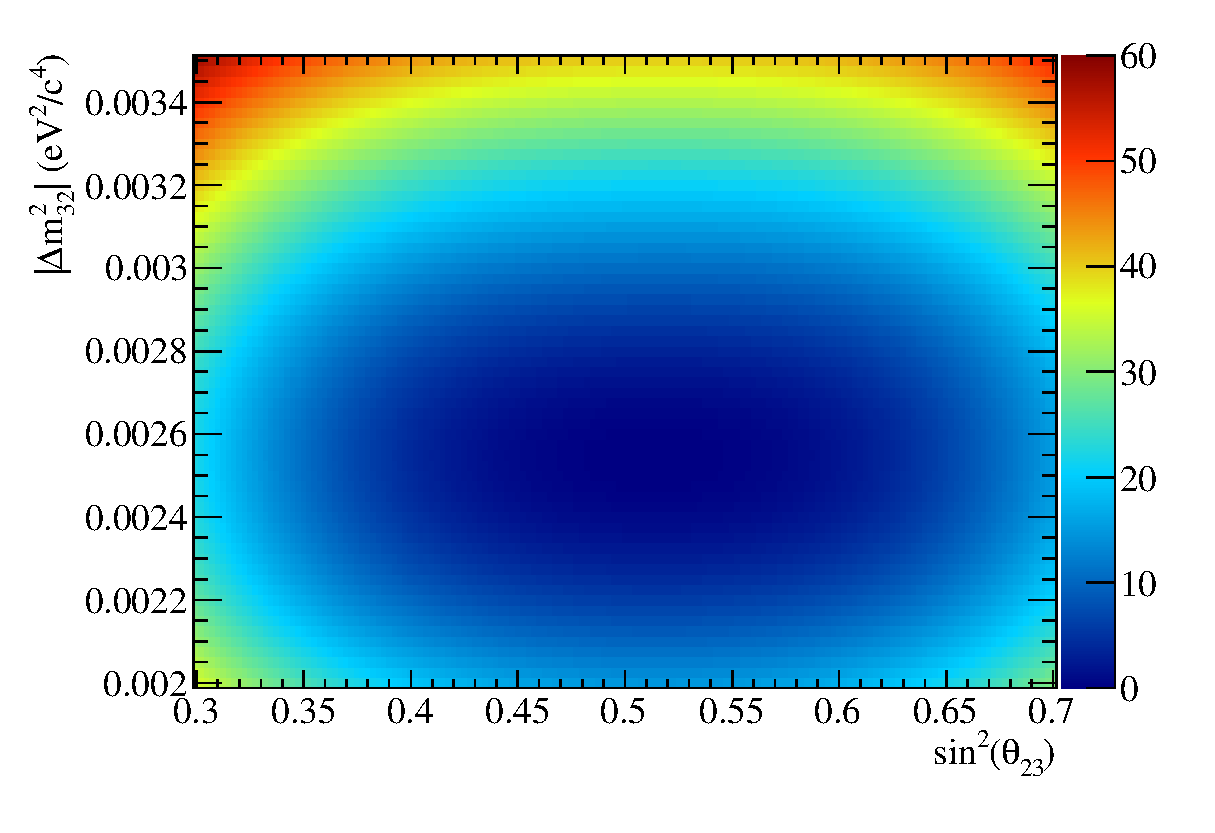
\includegraphics[width=21pc]{./images/data_fit/run4/run1-4_nuis4_sintheta_normal_run4_dchisq_maxz60}
\caption {
  $\Delta\chi^2$ surface from the fit of the Run 4 dataset.
  The normal mass hierarchy is assumed.
}
\label{fig:results_data4_chisq}
\end{minipage}
\end{figure*}

\clearpage

%...........................................................
%
% Const-dchi^2 contours 
%

\clearpage

\begin{figure*}[htb]
\center
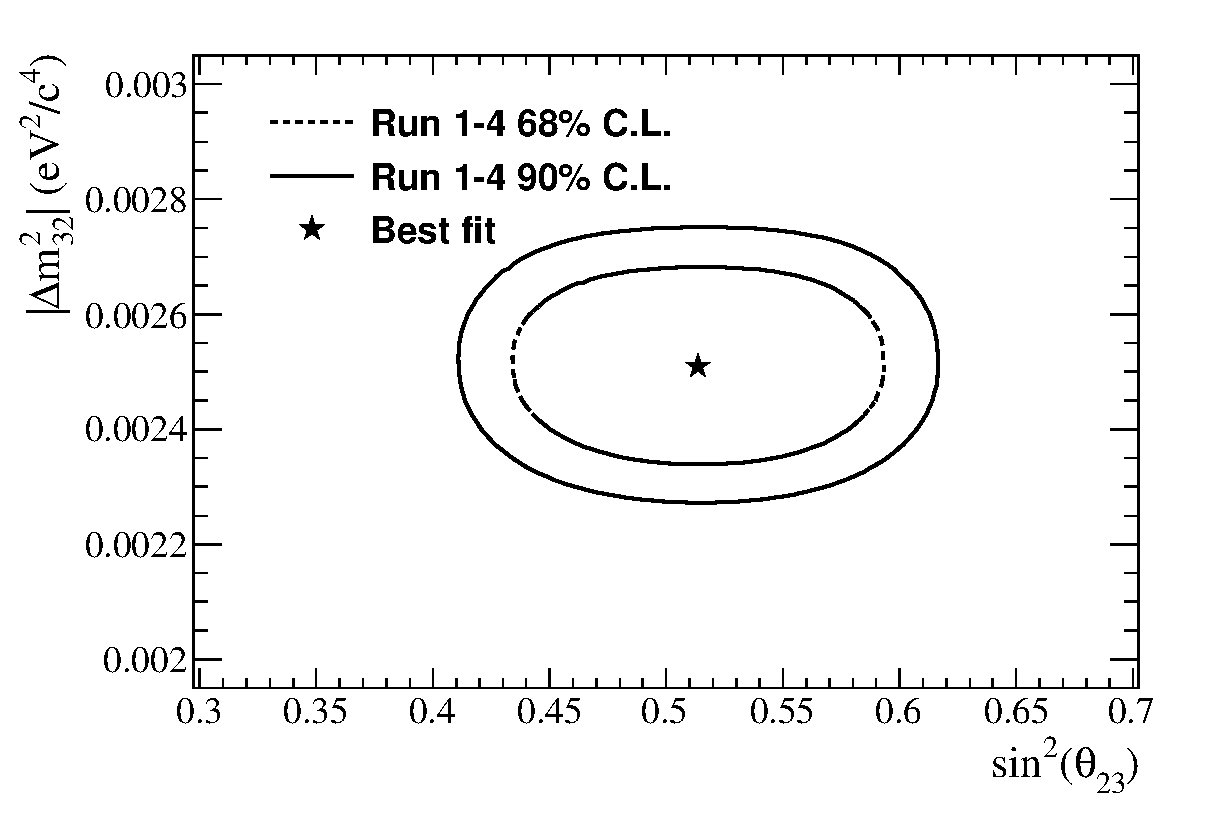
\includegraphics[width=30pc]{./images/data_fit/normal/run1-4_nuis4_sintheta_normal_contour}
\caption {
  68\% CL and 90\% CL allowed regions, 
  constructed with the constant-$\Delta\chi^{2}$ method,
  from the fit of the Run 1+2+3+4 dataset, 
  with the effects of statistical fluctuations and systematic variations being included. 
  The best-fit point is also shown.
  The normal mass hierarchy is assumed.
}
\label{fig:results_data1234_contour:normal}
\end{figure*}

\begin{figure*}[htb]
\center
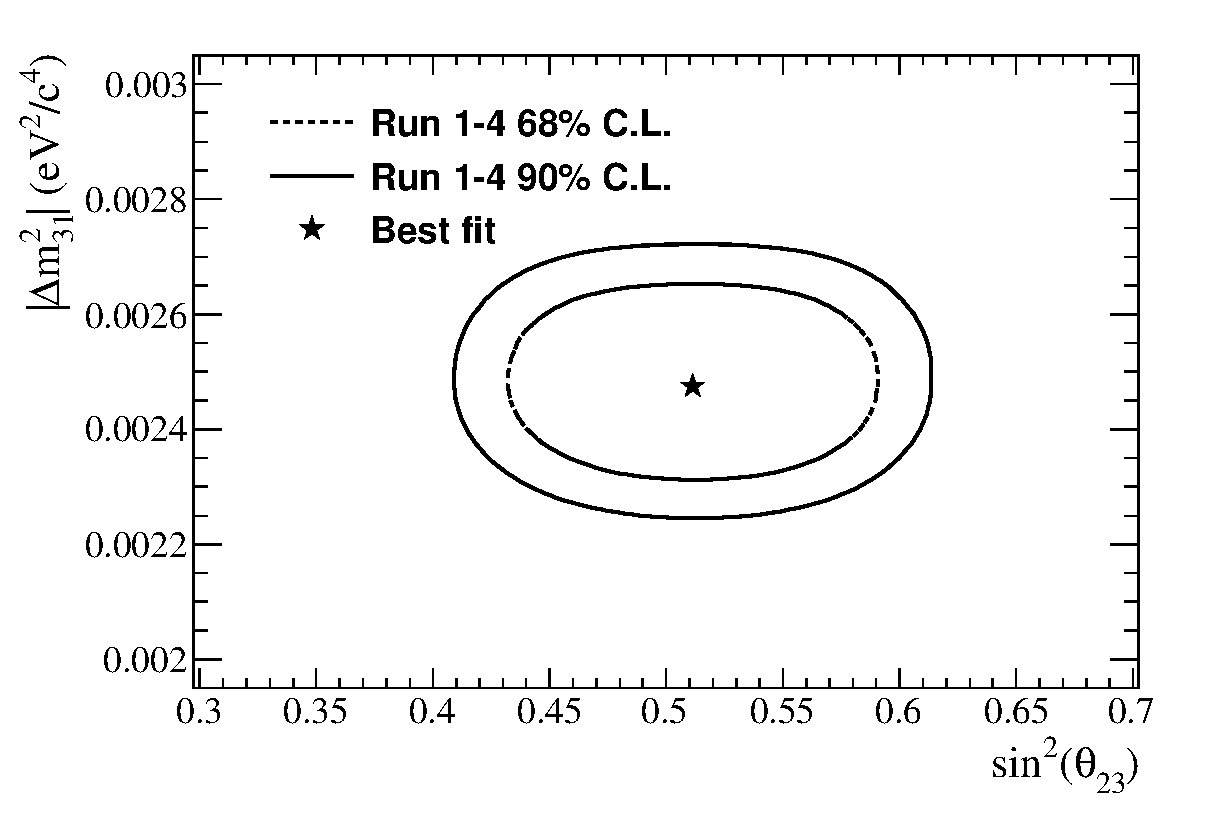
\includegraphics[width=30pc]{./images/data_fit/inverted31/run1-4_nuis4_sintheta_inverted31_contour}
\caption {
  68\% CL and 90\% CL allowed region, 
  constructed with the constant-$\Delta\chi^{2}$ method,
  from the fit of the Run 1+2+3+4 dataset,
  with the effects of statistical fluctuations and systematic variations being included.
  The best-fit point is also shown.
  The inverted mass hierarchy is assumed.
}
\label{fig:results_data1234_contour:inverted}
\end{figure*}

\begin{figure*}[htb]
\begin{minipage}[t]{0.48\linewidth}
\center
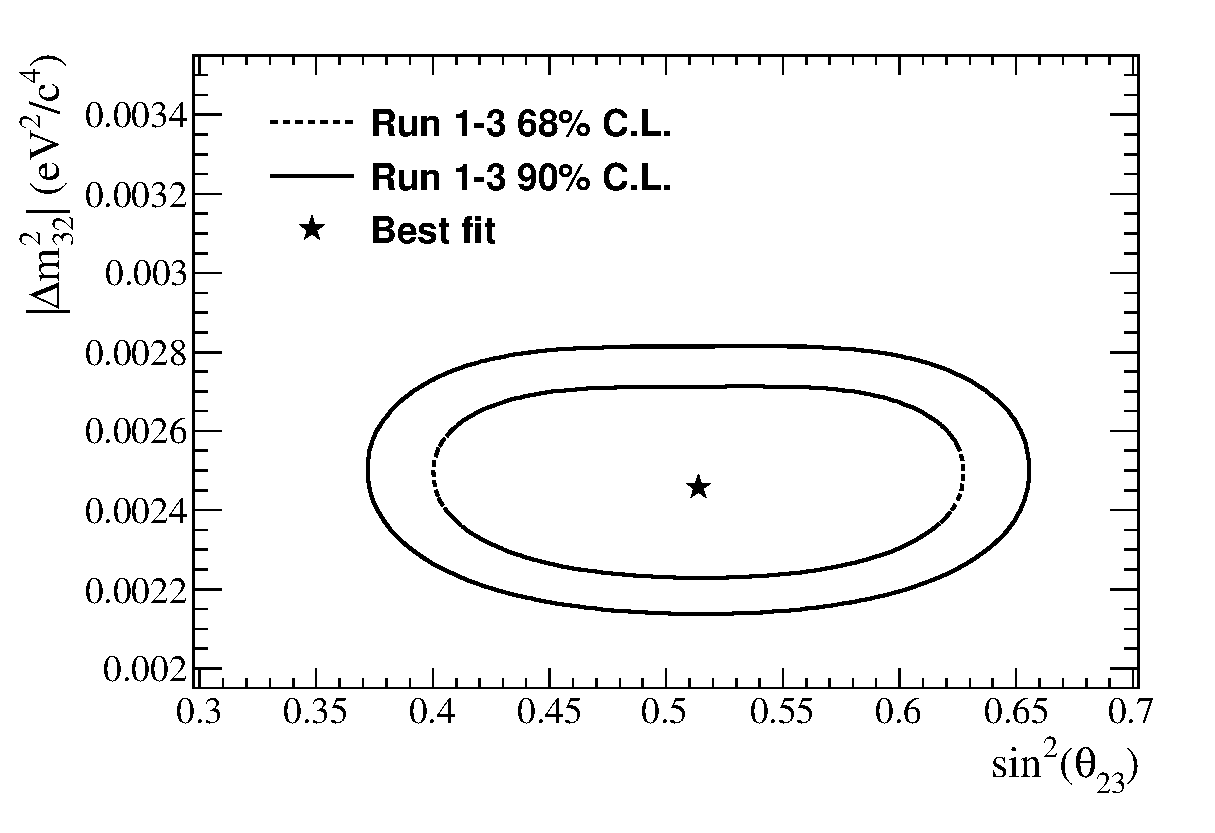
\includegraphics[width=20pc]{./images/data_fit/run123/run1-4_nuis4_sintheta_normal_run123_contour}
\caption {
  68\% CL and 90\% CL allowed regions,
  constructed with the constant-$\Delta\chi^{2}$ method,
  from the fit of the Run 1+2+3 dataset,
  with the effects of statistical fluctuations and systematic variations being included.
  The best-fit point is also shown.
  The normal mass hierarchy is assumed.
}
\label{fig:results_data123_contour}
\end{minipage}
\hspace{0.06\linewidth}
\begin{minipage}[t]{0.48\linewidth}
\center
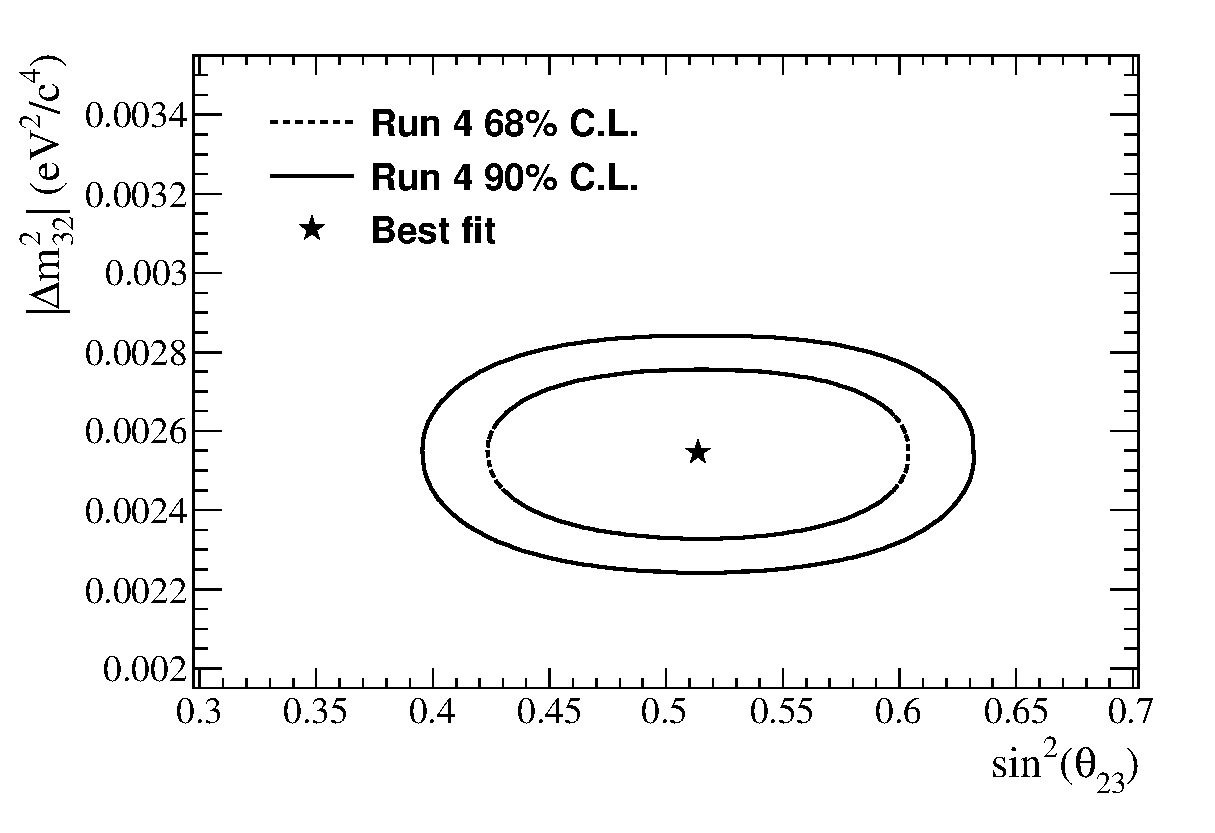
\includegraphics[width=20pc]{./images/data_fit/run4/run1-4_nuis4_sintheta_normal_run4_contour}
\caption {
  68\% CL and 90\% CL allowed regions,
  constructed with the constant-$\Delta\chi^{2}$ method,
  from the fit of the Run 4 dataset only,
  with the effects of statistical fluctuations and systematic variations being included.
  The best-fit point is also shown.
  The normal mass hierarchy is assumed.
}
\label{fig:results_data4_contour}
\end{minipage}
\end{figure*}

%...........................................................
%
% FC dchisq_critical surfaces
% 

\clearpage

\begin{figure*}[htb]
  \center
  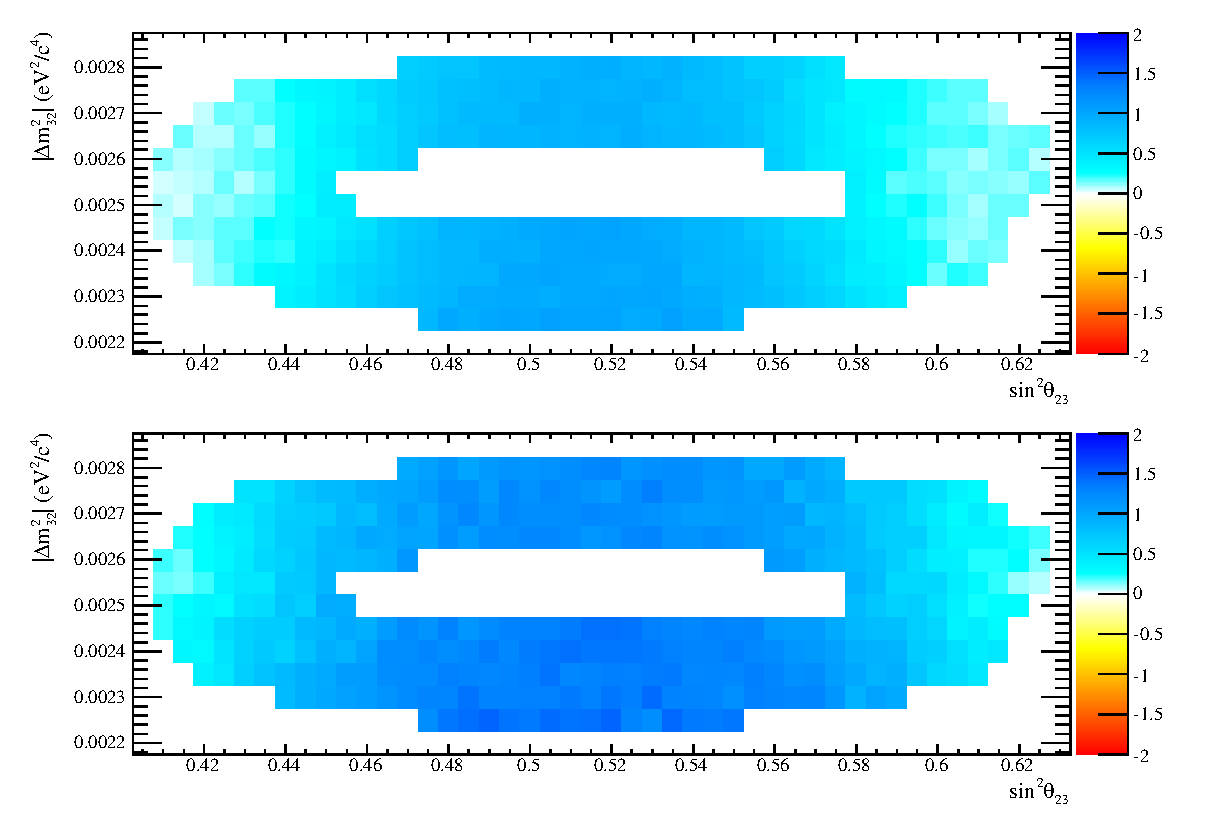
\includegraphics[width=42pc]{./images/fc_surface/FC_surfaces_normal}
  \caption {
    Difference between the $\Delta\chi^2_{critical}$ values obtained from the constant-$\Delta\chi^2$ method 
    and those from the Feldman-Cousins method \cite{FeldmanCousins} at confidence levels of 68\% (top) and 90\% (bottom),
    as a function of $\sin^{2}{\theta_{23}}$ and $|\Delta{m^{2}_{32}}|$.
    These surfaces were generated from an ensemble of toy MC experiments including both
    randomized systematic variations and statistical fluctuations.
    As expected from \cite{FeldmanCousins}, the Feldman-Cousins $\Delta\chi^{2}_{critical}$ values
    decrease as maximal $\nu_{\mu}$ disappearance at $\sin^{2}{\theta_{23}}$ $\approx$ 0.513 is approached.
    The normal mass hierarchy is assumed.
    $\Delta\chi^2_{critical}$ is only calculated for values of 
    $\sin^{2}{\theta_{23}}$ and $|\Delta{m^{2}_{32}}|$
    that affect the 68\% and 90\% confidence contours. 
    }
  \label{fig:fc_dchisqcrit_2d:normal}
\end{figure*}

%.......

\clearpage

\begin{figure*}[htb]
  \center
  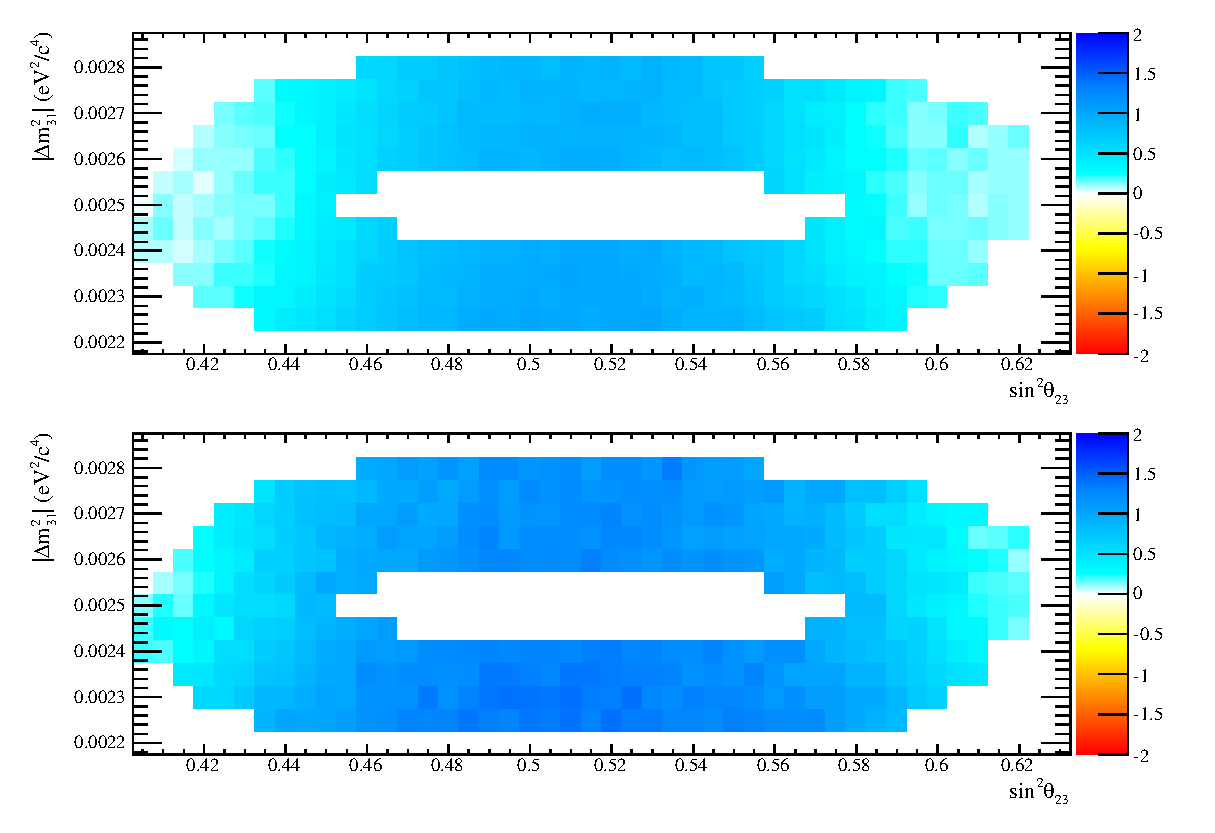
\includegraphics[width=42pc]{./images/fc_surface/FC_surfaces_inverted31}
  \caption {
    Difference between the $\Delta\chi^2_{critical}$ values obtained from the constant-$\Delta\chi^2$ method
    and those from the Feldman-Cousins method \cite{FeldmanCousins} at confidence levels of 68\% (top) and 90\% (bottom),
    as a function of $\sin^{2}{\theta_{23}}$ and $|\Delta{m^{2}_{31}}|$.
    These surfaces were generated from an ensemble of toy MC experiments including both
    randomized systematic variations and statistical fluctuations.
    As expected from \cite{FeldmanCousins}, the Feldman-Cousins $\Delta\chi^{2}_{critical}$ values
    decrease as maximal $\nu_{\mu}$ disappearance at $\sin^{2}{\theta_{23}}$ $\approx$ 0.513 is approached.
    The inverted mass hierarchy is assumed.
    $\Delta\chi^2_{critical}$ is only calculated for values of
    $\sin^{2}{\theta_{23}}$ and $|\Delta{m^{2}_{32}}|$
    that affect the 68\% and 90\% confidence contours.
  }
  \label{fig:fc_dchisqcrit_2d:inverted}
\end{figure*}

%...........................................................
%
% FC dchisq_critical surface projections
% 

\begin{figure*}[htb]
  \center
  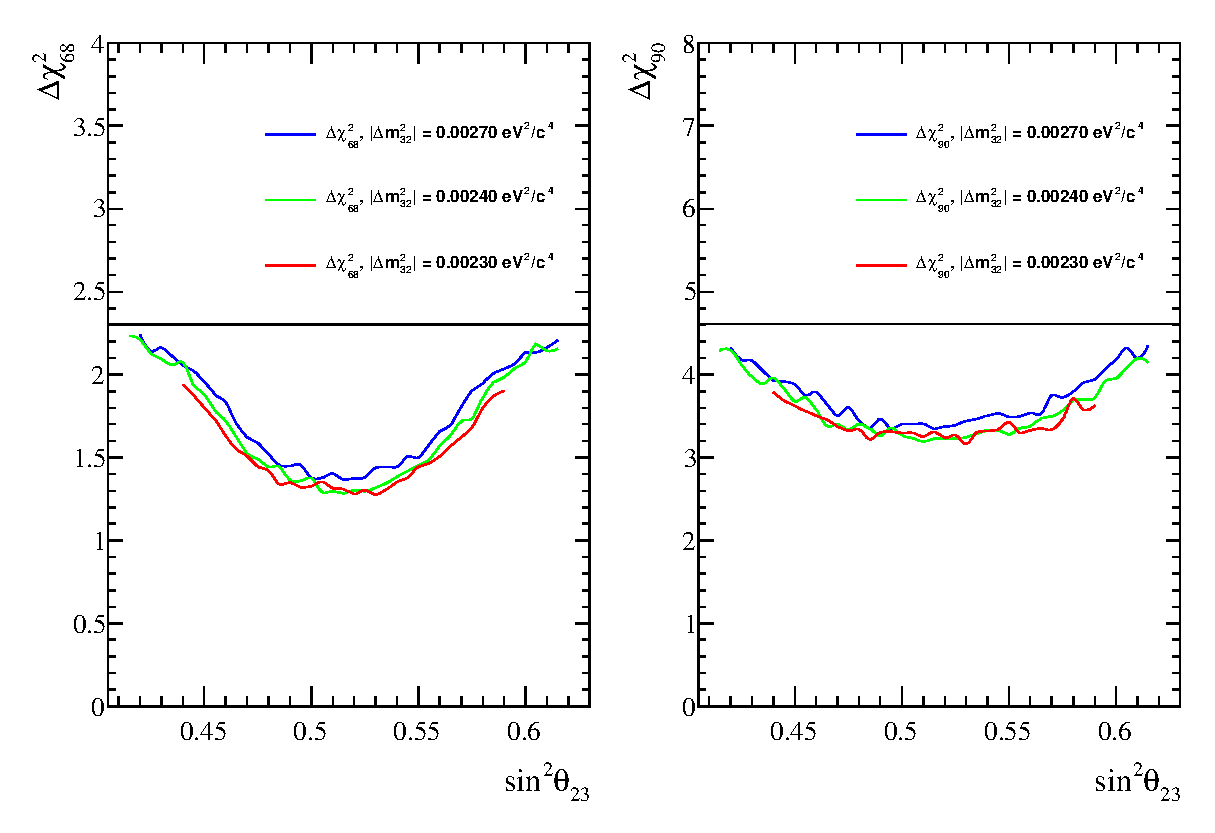
\includegraphics[width=30pc]{./images/fc_surface/FC_slice_mixing_normal}
  \caption {
    1-dimensional slices through the 68\% (left) and 90\% (right) 2-dimensional surfaces of 
    Feldman-Cousins $\Delta\chi^{2}_{critical}$ values
    as a function of $\sin^{2}{\theta_{23}}$ for 3 different values of $|\Delta{m^{2}_{32}}|$
    (2.3$\times$10$^{-3}$ eV$^{2}/c^{4}$,
    2.4$\times$10$^{-3}$ eV$^{2}/c^{4}$ and
    2.7$\times$10$^{-3}$ eV$^{2}/c^{4}$).
    The $\Delta\chi^{2}_{critical}$ values were calculated
    from an ensemble of toy MC experiments, for an exposure of 6.5700$\times$10$^{20}$ POT,
    including both randomized systematic variations and statistical fluctuations.
    For comparison, the canonical value used in the constant-$\Delta\chi^{2}$
    method is also shown as a horizontal line.
    The normal mass hierarchy is assumed.
    $\Delta\chi^2_{critical}$ is only calculated for values of
    $\sin^{2}{\theta_{23}}$ and $|\Delta{m^{2}_{32}}|$
    that affect the 68\% and 90\% confidence contours.
  }
  \label{fig:fc_dchisqcrit_slice_mixing:normal}
\end{figure*}

%.......

\begin{figure*}[htb]
  \center
  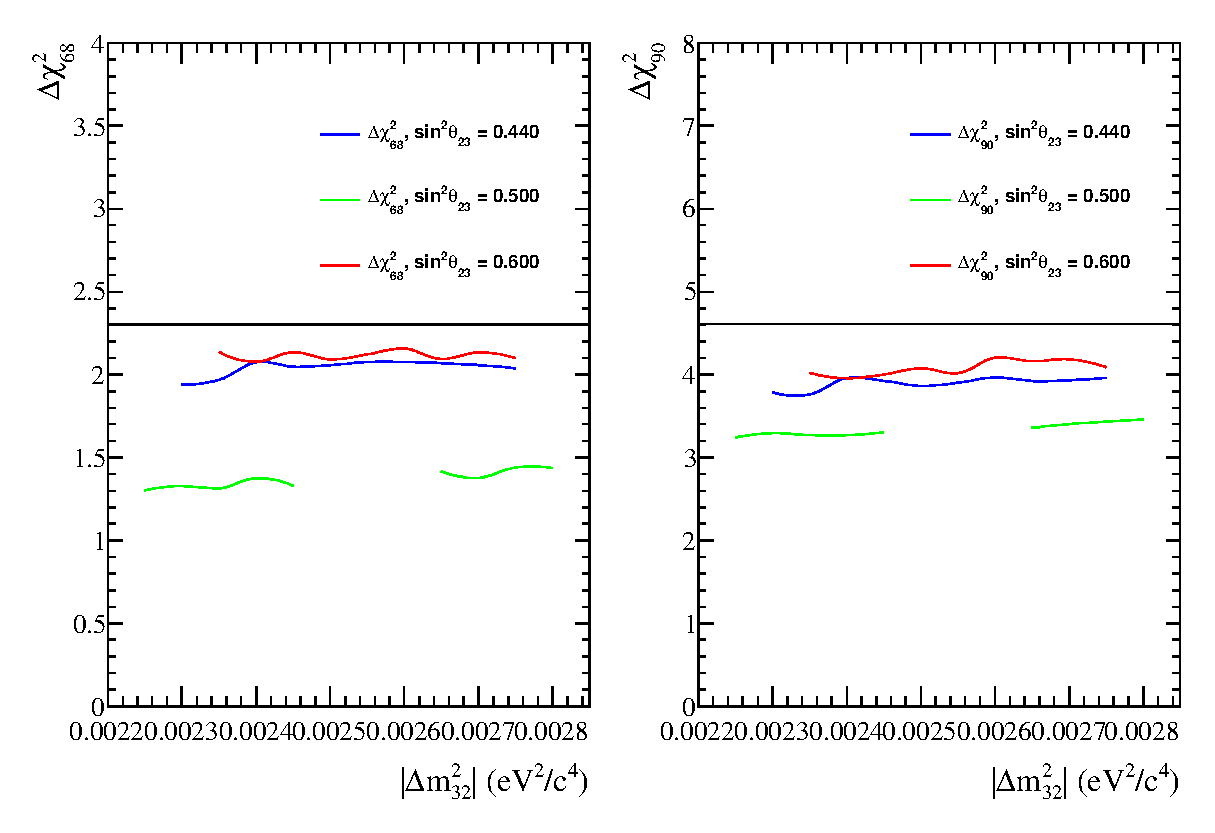
\includegraphics[width=30pc]{./images/fc_surface/FC_slice_dmsq_normal}
  \caption {
    1-dimensional slices through the 68\% (left) and 90\% (right) 2-dimensional surfaces of
    Feldman-Cousins $\Delta\chi^{2}_{critical}$ values
    as a function of $|\Delta{m^{2}_{32}}|$ for 3 different values of $\sin^{2}{\theta_{23}}$
    (0.44, 0.50 and 0.60).
    The $\Delta\chi^{2}_{critical}$ values were calculated
    from an ensemble of toy MC experiments, for an exposure of 6.5700$\times$10$^{20}$ POT,
    including both randomized systematic variations and statistical fluctuations.
    For comparison, the canonical value used in the constant-$\Delta\chi^{2}$
    method is also shown as a horizontal line.
    The normal mass hierarchy is assumed.
    $\Delta\chi^2_{critical}$ is only calculated for values of
    $\sin^{2}{\theta_{23}}$ and $|\Delta{m^{2}_{32}}|$
    that affect the 68\% and 90\% confidence contours.
  }
  \label{fig:fc_dchisqcrit_slice_dmsq:normal}
\end{figure*}

%.......

\begin{figure*}[htb]
  \center
  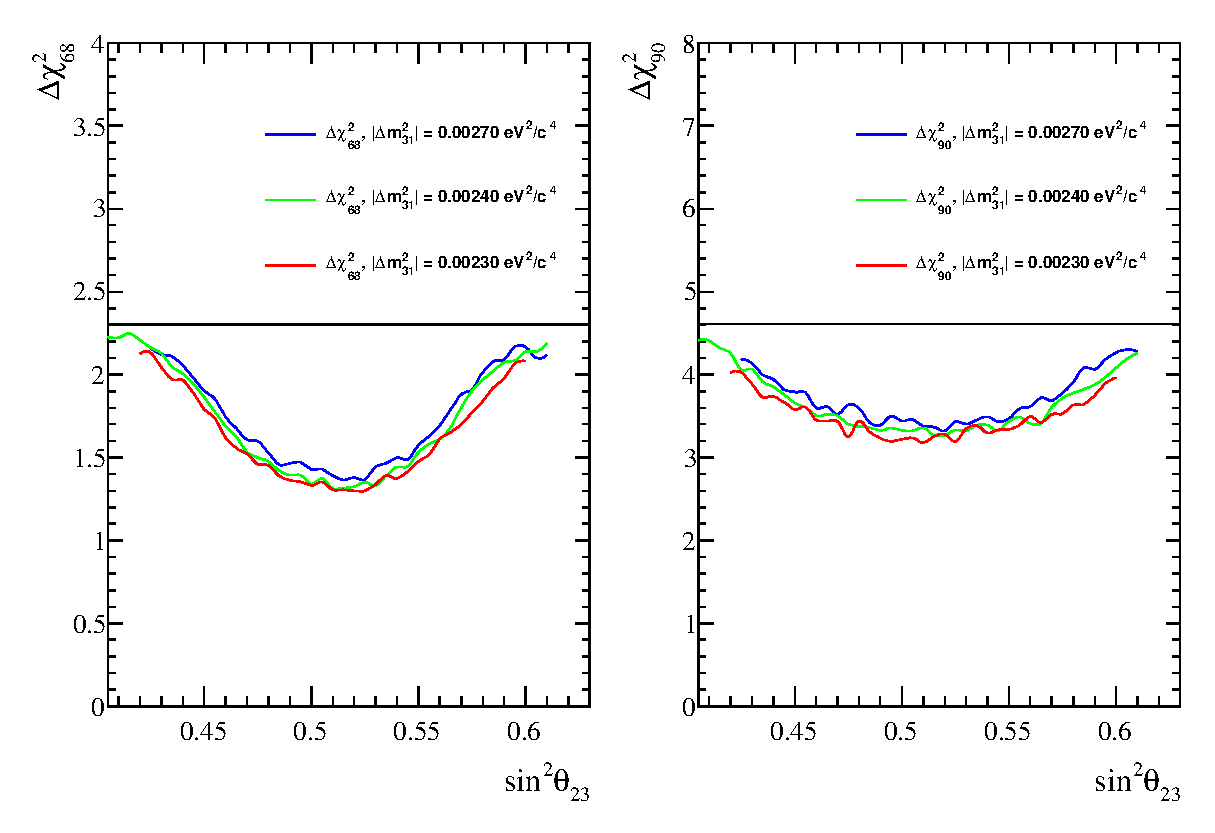
\includegraphics[width=30pc]{./images/fc_surface/FC_slice_mixing_inverted31}
  \caption {
    1-dimensional slices through the 68\% (left) and 90\% (right) 2-dimensional surfaces of
    Feldman-Cousins $\Delta\chi^{2}_{critical}$ values
    as a function of $\sin^{2}{\theta_{23}}$ for 3 different values of $|\Delta{m^{2}_{31}}|$
    (2.3$\times$10$^{-3}$ eV$^{2}/c^{4}$,
    2.4$\times$10$^{-3}$ eV$^{2}/c^{4}$ and
    2.7$\times$10$^{-3}$ eV$^{2}/c^{4}$).
    The $\Delta\chi^{2}_{critical}$ values were calculated
    from an ensemble of toy MC experiments, for an exposure of 6.5700$\times$10$^{20}$ POT,
    including both randomized systematic variations and statistical fluctuations.
    For comparison, the canonical value used in the constant-$\Delta\chi^{2}$
    method is also shown as a horizontal line.
    The inverted mass hierarchy is assumed.
    $\Delta\chi^2_{critical}$ is only calculated for values of
    $\sin^{2}{\theta_{23}}$ and $|\Delta{m^{2}_{31}}|$
    that affect the 68\% and 90\% confidence contours.
  }
  \label{fig:fc_dchisqcrit_slice_mixing:inverted}
\end{figure*}

%.......

\begin{figure*}[htb]
  \center
  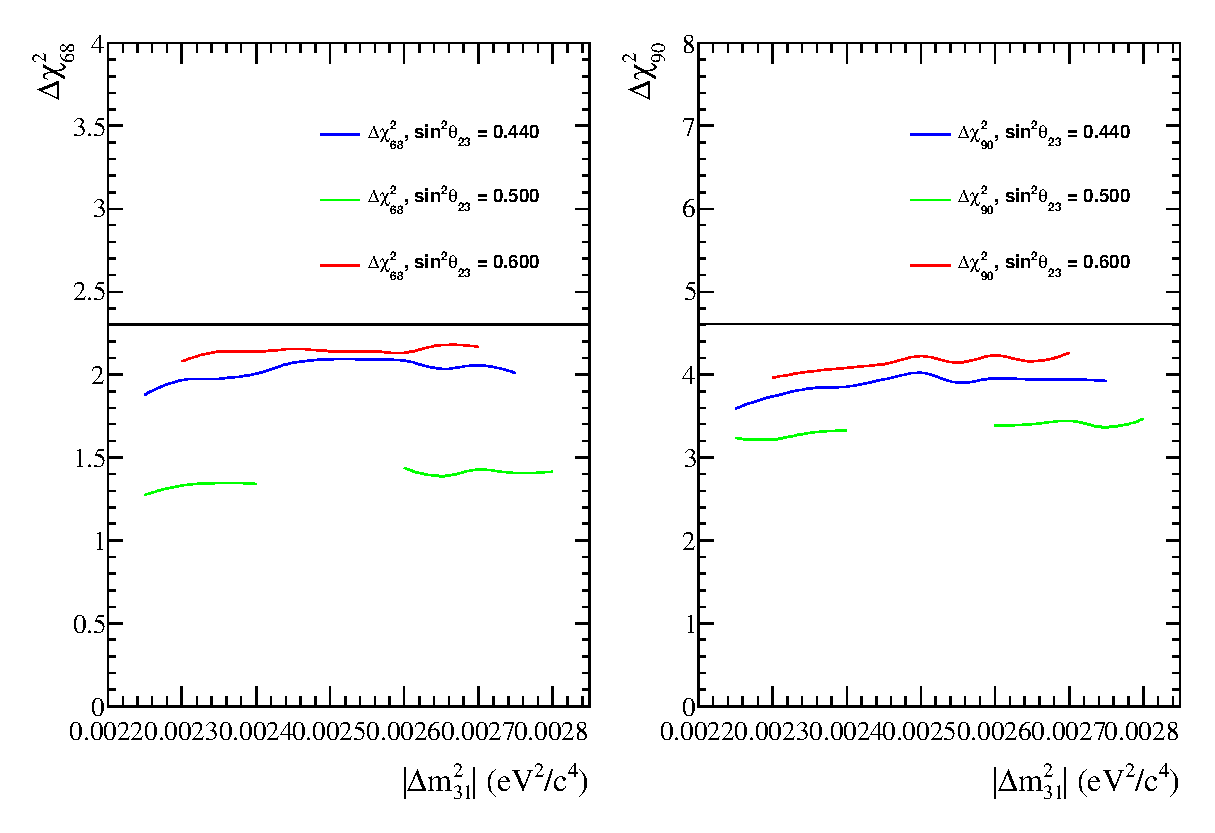
\includegraphics[width=30pc]{./images/fc_surface/FC_slice_dmsq_inverted31}
  \caption {
    1-dimensional slices through the 68\% (left) and 90\% (right) 2-dimensional surfaces of
    Feldman-Cousins $\Delta\chi^{2}_{critical}$ values
    as a function of $|\Delta{m^{2}_{31}}|$ for 3 different values of $\sin^{2}{\theta_{23}}$
    (0.44, 0.50 and 0.60).
    The $\Delta\chi^{2}_{critical}$ values were calculated
    from an ensemble of toy MC experiments, for an exposure of 6.5700$\times$10$^{20}$ POT,
    including both randomized systematic variations and statistical fluctuations.
    For comparison, the canonical value used in the constant-$\Delta\chi^{2}$
    method is also shown as a horizontal line.
    The inverted mass hierarchy is assumed.
    $\Delta\chi^2_{critical}$ is only calculated for values of
    $\sin^{2}{\theta_{23}}$ and $|\Delta{m^{2}_{31}}|$
    that affect the 68\% and 90\% confidence contours.
  }
  \label{fig:fc_dchisqcrit_slice_dmsq:inverted}
\end{figure*}


%...........................................................
%
% FC contours 
% 

\begin{figure*}[htb]
  \center
  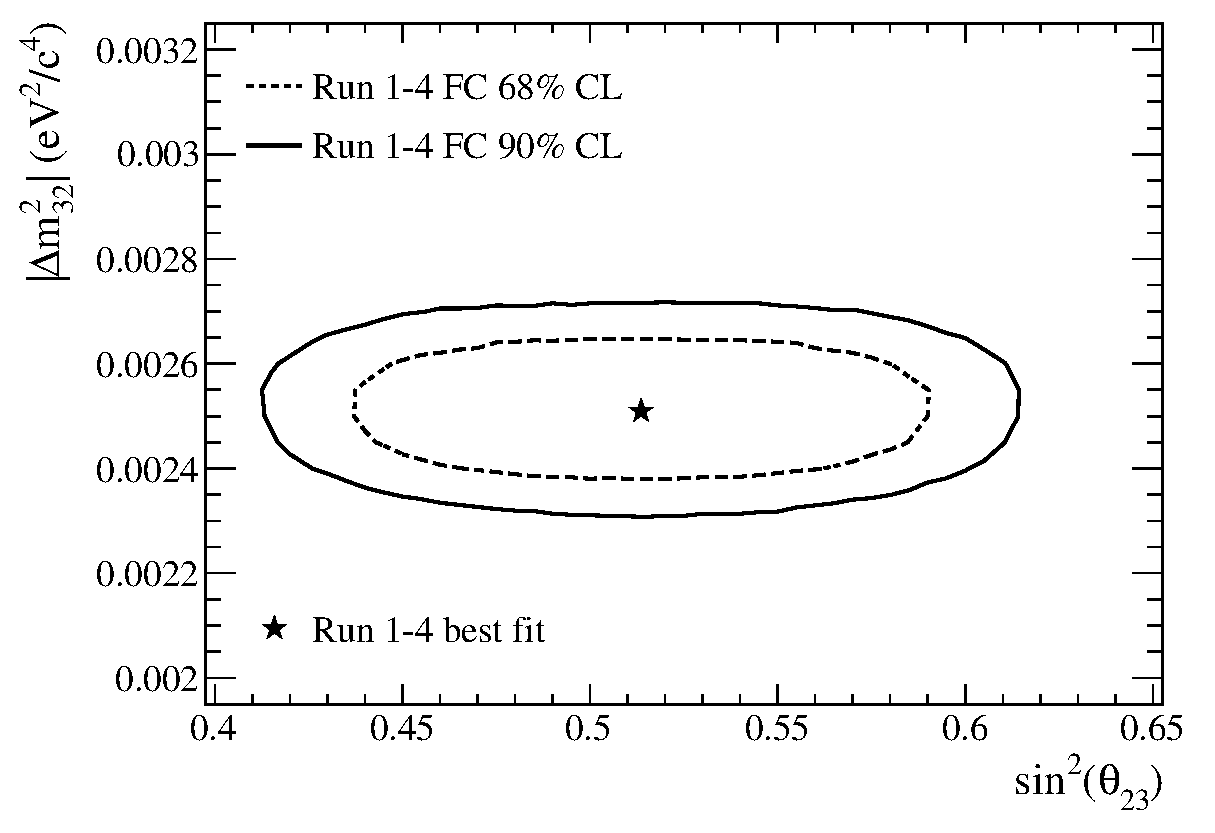
\includegraphics[width=35pc]{./images/data_fit/fc/contour_compare_normal_fconly}
  \caption {
    68\% CL and 90\% CL allowed regions, 
    constructed with the method of Feldman and Cousins,
    from the fit of the Run 1+2+3+4 dataset,
    with the effects of statistical fluctuations and systematic variations being included.
    The best-fit point is also shown.
    The normal mass hierarchy is assumed.
  }
  \label{fig:results_data1234_fc_contour:normal}
\end{figure*}

\begin{figure*}[htb]
  \center
  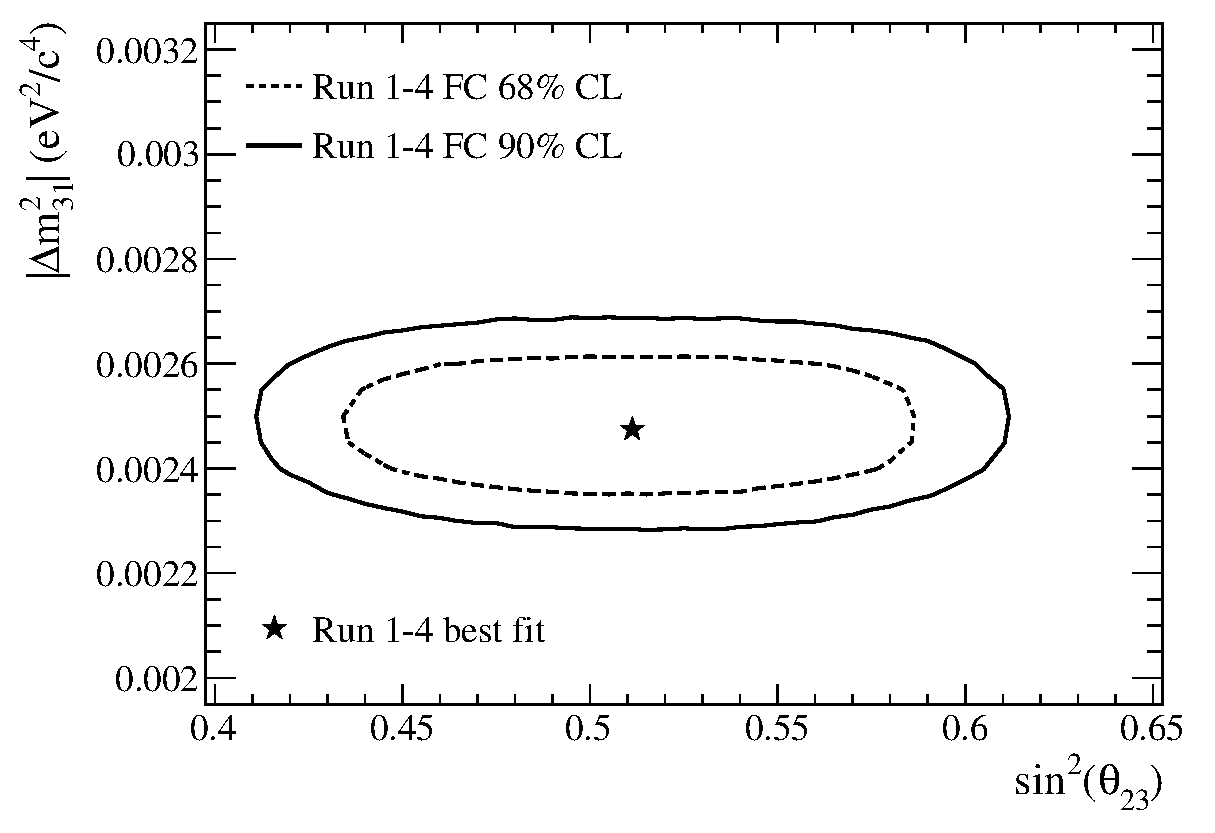
\includegraphics[width=35pc]{./images/data_fit/fc/contour_compare_inverted31_fconly}
  \caption {
    68\% CL and 90\% CL allowed regions, 
    constructed with the method of Feldman and Cousins,
    from the fit to the Run 1+2+3+4 dataset,
    with the effects of statistical fluctuations and systematic variations being included.
    The best-fit point is also shown.
    The inverted mass hierarchy is assumed.
  }
  \label{fig:results_data1234_fc_contour:inverted}
\end{figure*}

\clearpage

%...........................................................                                                                                                                          
%                                                                                                                                                                             
% Profile \Delta\chisquare plots & Table summarizing 1D limits                                                                                                                       
%

\begin{figure*}[htb]
  \begin{minipage}[t]{0.96\linewidth}
    \center
    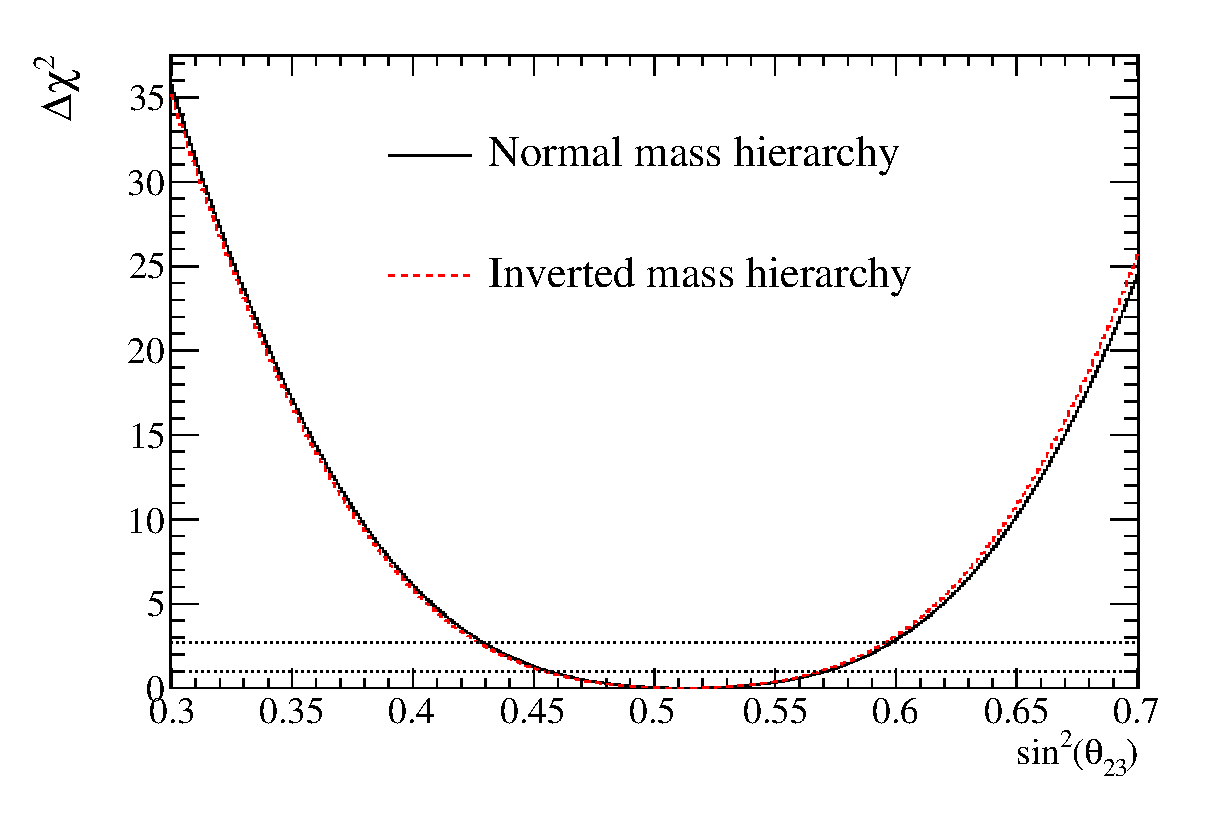
\includegraphics[width=30pc]{./images/data_fit/compare/dchisq_profiles_mix23}
    \caption {
      Profile $\Delta\chi^2$, as a function of $\sin^{2}\theta_{23}$,
      from the 2-parameter fits of the Run 1+2+3+4 dataset.
      The 68\% and 90\% critical constant-$\Delta\chi^{2}$ values
      for one degree of freedom
      are shown as horizontal dotted lines.
    }
    \label{fig:results_marg_dchisq_dmsq_normalinverted}
  \end{minipage}
  \vfill
  \begin{minipage}[t]{0.96\linewidth}
    \center
    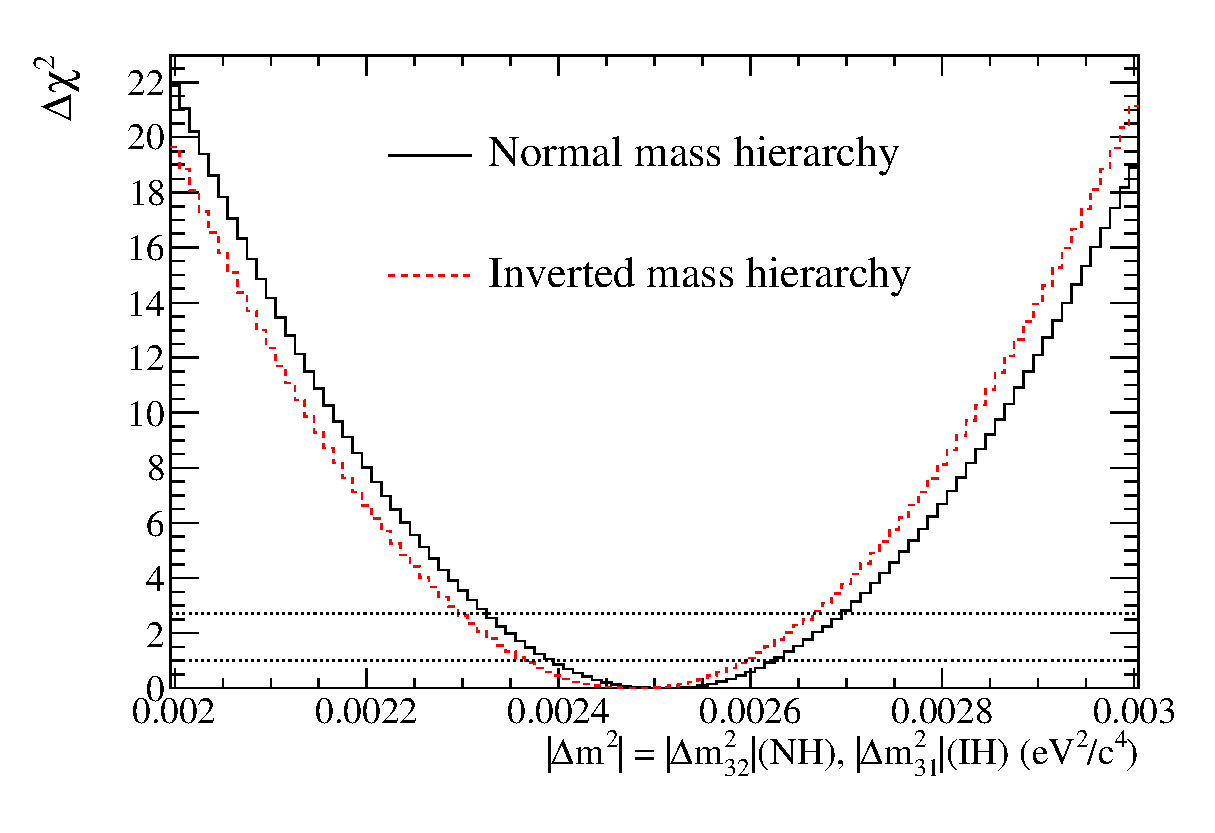
\includegraphics[width=30pc]{./images/data_fit/compare/dchisq_profiles_dm32sq}
    \caption {
      Profile $\Delta\chi^2$, as a function of $|\Delta m^{2}_{32}|$ for the normal mass hierarchy
      and of $|\Delta m^{2}_{31}|$ for the inverted mass hierarchy,
      from the 2-parameter fits of the Run 1+2+3+4 dataset.
      The 68\% and 90\% critical constant-$\Delta\chi^{2}$ values
      for one degree of freedom
      are shown as horizontal dotted lines.
    }
    \label{fig:results_marg_dchisq_sinsq_normalinverted}
  \end{minipage}
\end{figure*}

\begin{figure*}[htb]
\center
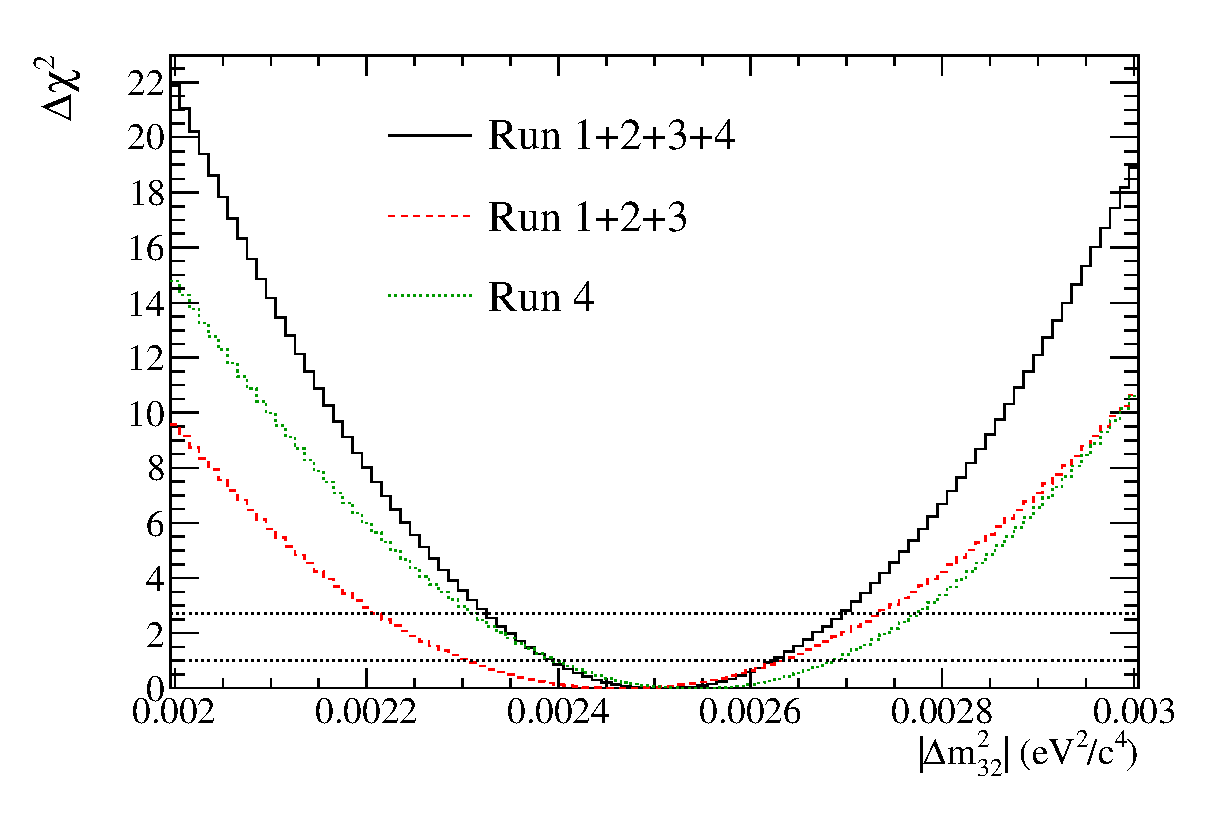
\includegraphics[width=30pc]{./images/data_fit/compare/dchisq_profiles3_dm32sq_sepruns}
\caption {
  Profile $\Delta\chi^2$, as a function of $|\Delta m^{2}_{32}|$,
  from the 2-parameter fits of the Run 1+2+3+4, Run 1+2+3 and Run 4 datasets.
  The normal mass hierarchy is assumed.
}
\label{fig:results_marg_dchisq_dmsq_all3}
\end{figure*}

\begin{figure*}[htb]
\center
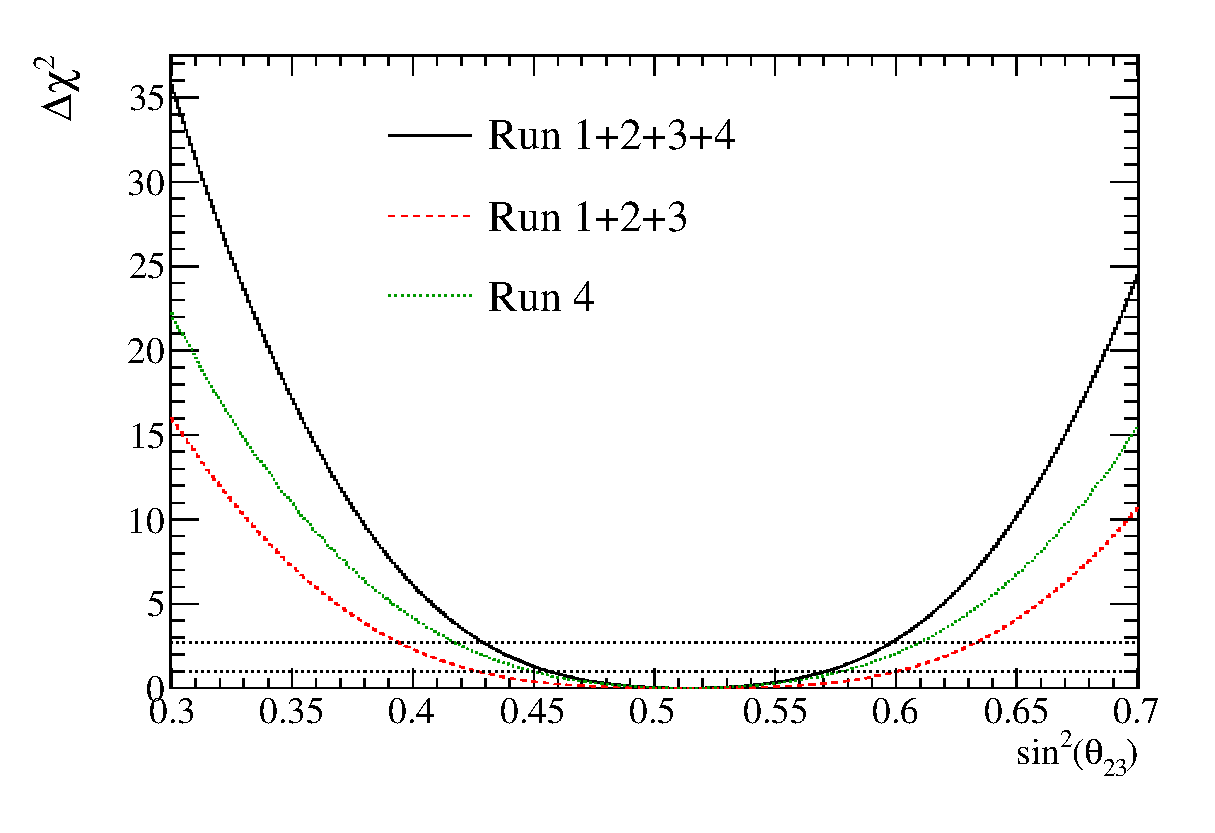
\includegraphics[width=30pc]{./images/data_fit/compare/dchisq_profiles3_mix23_sepruns}
\caption {
  Profile $\Delta\chi^2$, as a function of $\sin^{2}\theta_{23}$,
  from the 2-parameter fits of the Run 1+2+3+4, Run 1+2+3 and Run 4 datasets.
  The normal mass hierarchy is assumed.
}
\label{fig:results_marg_dchisq_sinsq_all3}
\end{figure*}

\begin{figure*}[htb]
  \begin{minipage}[t]{0.96\linewidth}
    \center
    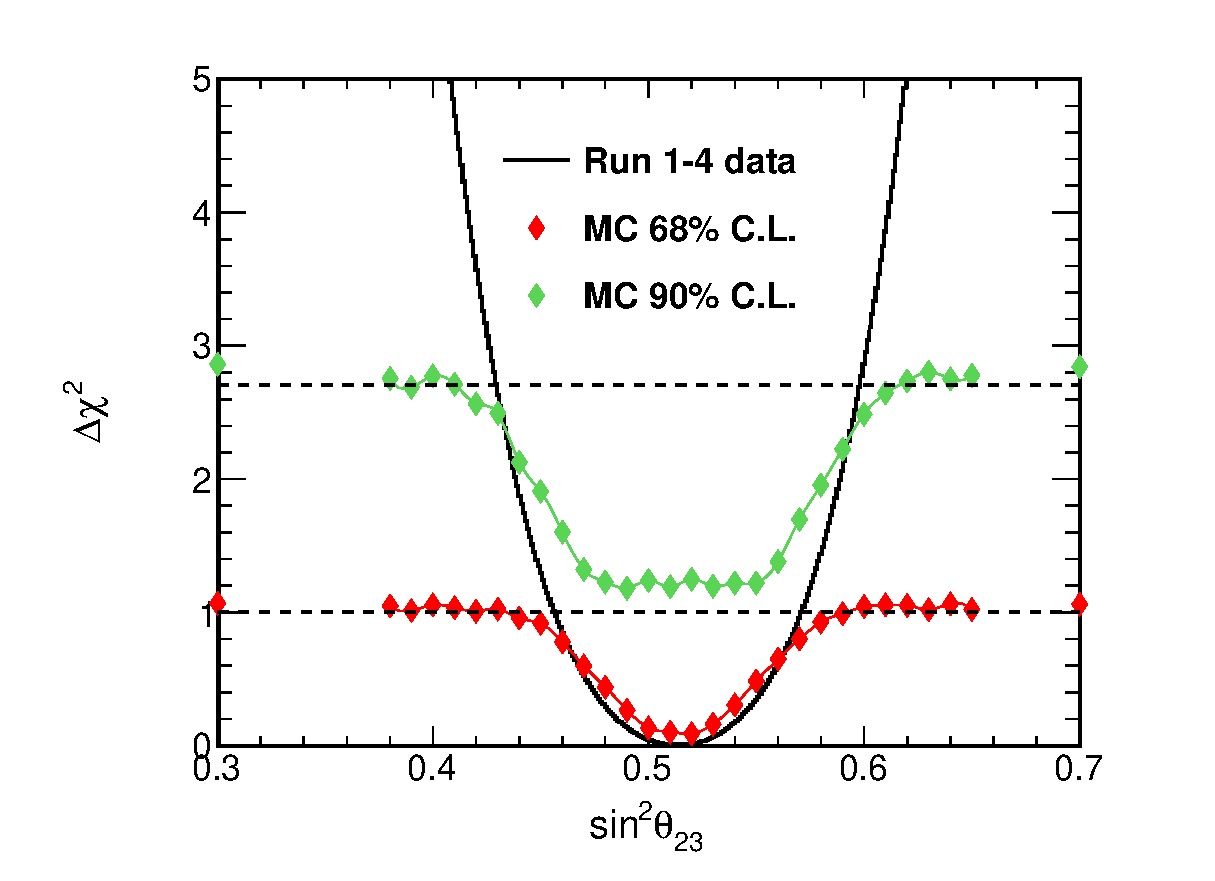
\includegraphics[width=30pc]{./images/data_fit/normal/run1-4_nuis4_sintheta_normal_1DFC_interval}
    \caption {
     Comparison between the 1D $\Delta \chi^{2}$ from the fit of the Run 1+2+3+4 data and the Monte Carlo estimation of the
     1D 68\% and 90\% critical values of $\Delta \chi^{2}$ as a function of $\sin^{2}\theta_{23}$. Each MC
     critical value is obtained from 10000 toy experiments with systematic variations and statistical fluctuations; these
     critical values are fitted with cubic splines. The normal mass hierarchy is assumed.
     The canonical constant-$\Delta \chi^{2}$ 68\% and 90\% critical values for one degree of freedom are shown as dashed lines.
    }
    \label{fig:results_1D_dchisq_sinsq_normal}
  \end{minipage}
  \vfill
  \begin{minipage}[t]{0.96\linewidth}
    \center
    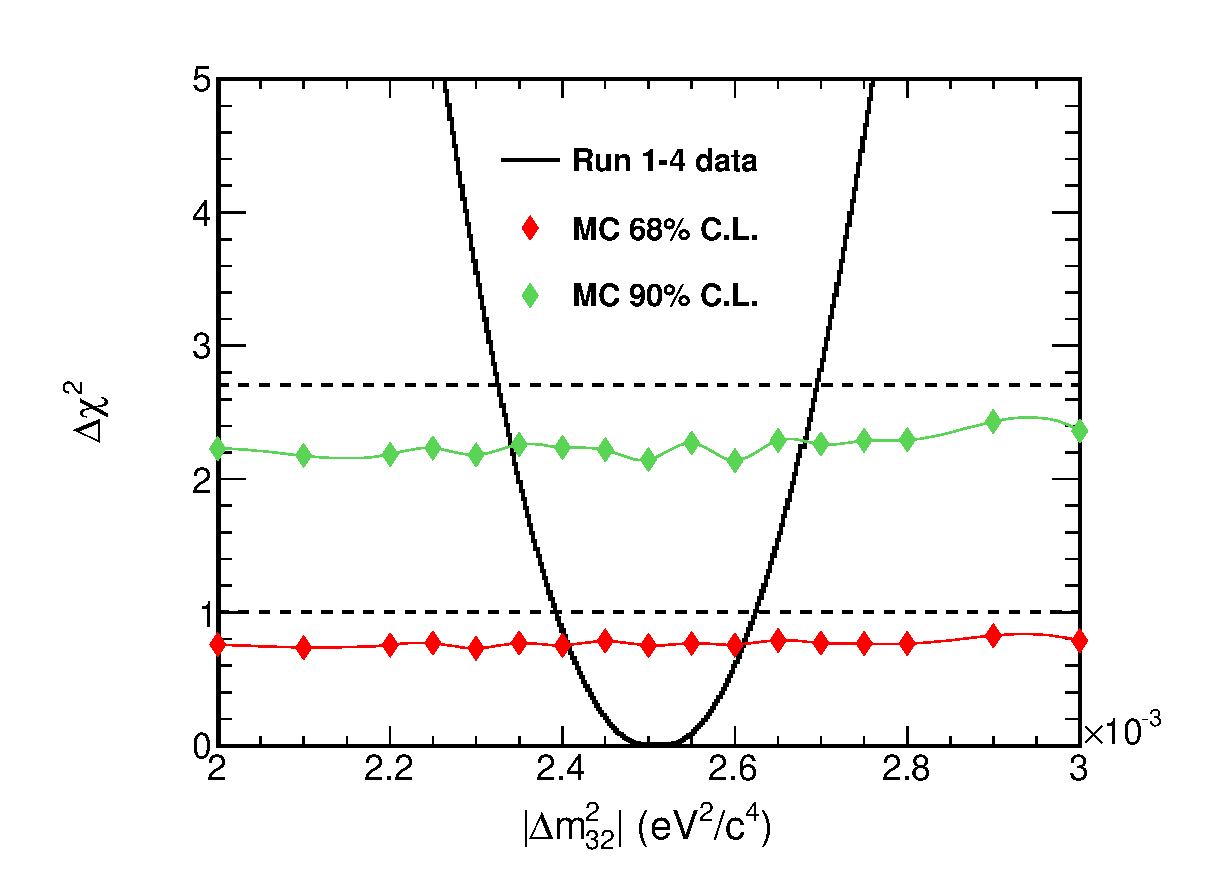
\includegraphics[width=30pc]{./images/data_fit/normal/run1-4_nuis4_dm32sq_normal_1DFC_interval}
    \caption {
     Comparison between the 1D $\Delta \chi^{2}$ from the fit of the Run 1+2+3+4 data and the Monte Carlo estimation of the
     1D 68\% and 90\% critical values of $\Delta \chi^{2}$ as a function of $|\Delta m^{2}_{32}|$. Each MC
     critical value is obtained from 10000 toy experiments with systematic variations and statistical fluctuations; these
     critical values are fitted with cubic splines. The normal mass hierarchy is assumed.
     The canonical constant-$\Delta \chi^{2}$ 68\% and 90\% critical values for one degree of freedom are shown as dashed lines.
    }
    \label{fig:results_1D_dchisq_dm32sq_normal}
  \end{minipage}
\end{figure*}

\begin{figure*}[htb]
  \begin{minipage}[t]{0.96\linewidth}
    \center
    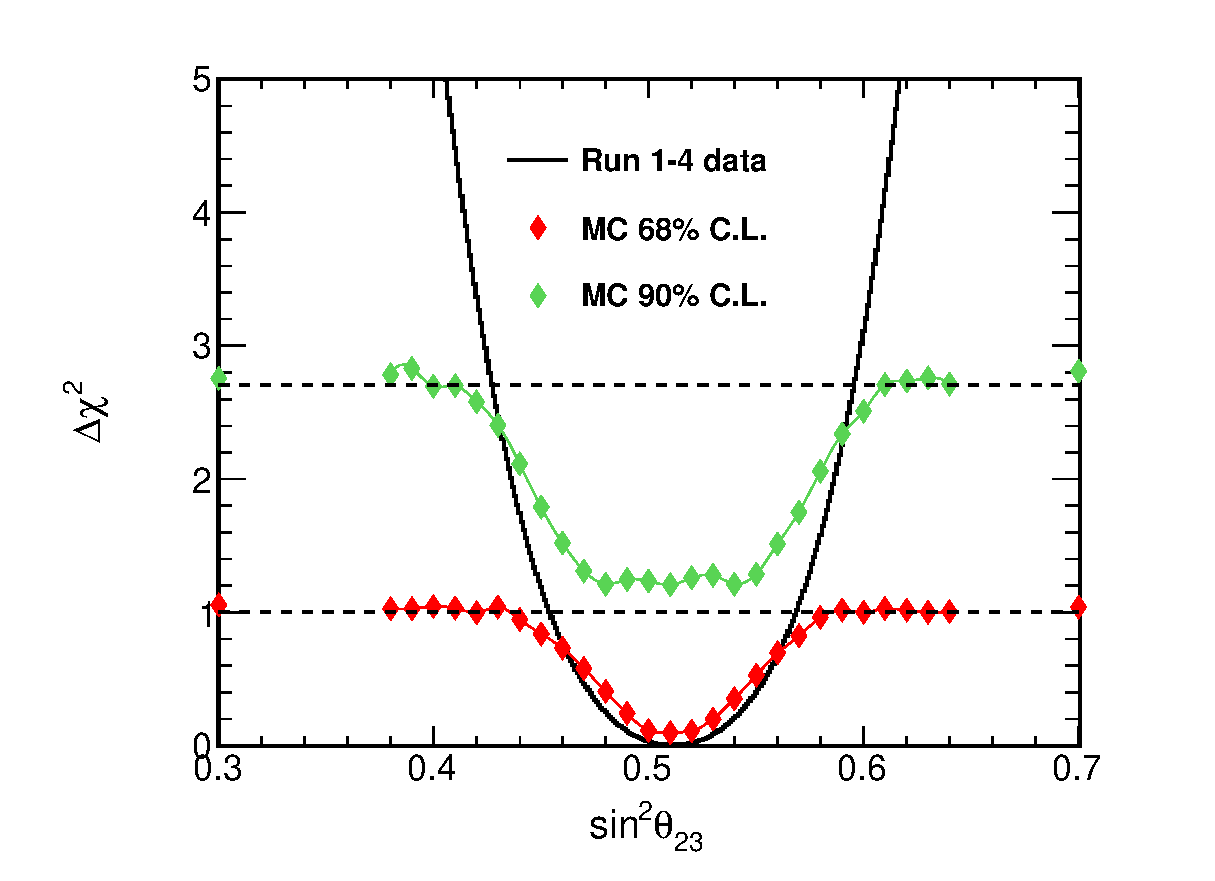
\includegraphics[width=30pc]{./images/data_fit/inverted31/run1-4_nuis4_mixing23_inverted_1DFC_interval}
    \caption {
     Comparison between the 1D $\Delta \chi^{2}$ from the fit of the Run 1+2+3+4 data and the Monte Carlo estimation of the
     1D 68\% and 90\% critical values of $\Delta \chi^{2}$ as a function of $\sin^{2}\theta_{23}$. Each MC
     critical value is obtained from 10000 toy experiments with systematic variations and statistical fluctuations; these
     critical values are fitted with cubic splines. The inverted mass hierarchy is assumed.
     The canonical constant-$\Delta \chi^{2}$ 68\% and 90\% critical values for one degree of freedom are shown as dashed lines.
    }
    \label{fig:results_1D_dchisq_sinsq_inverted}
  \end{minipage}
  \vfill
  \begin{minipage}[t]{0.96\linewidth}
    \center
    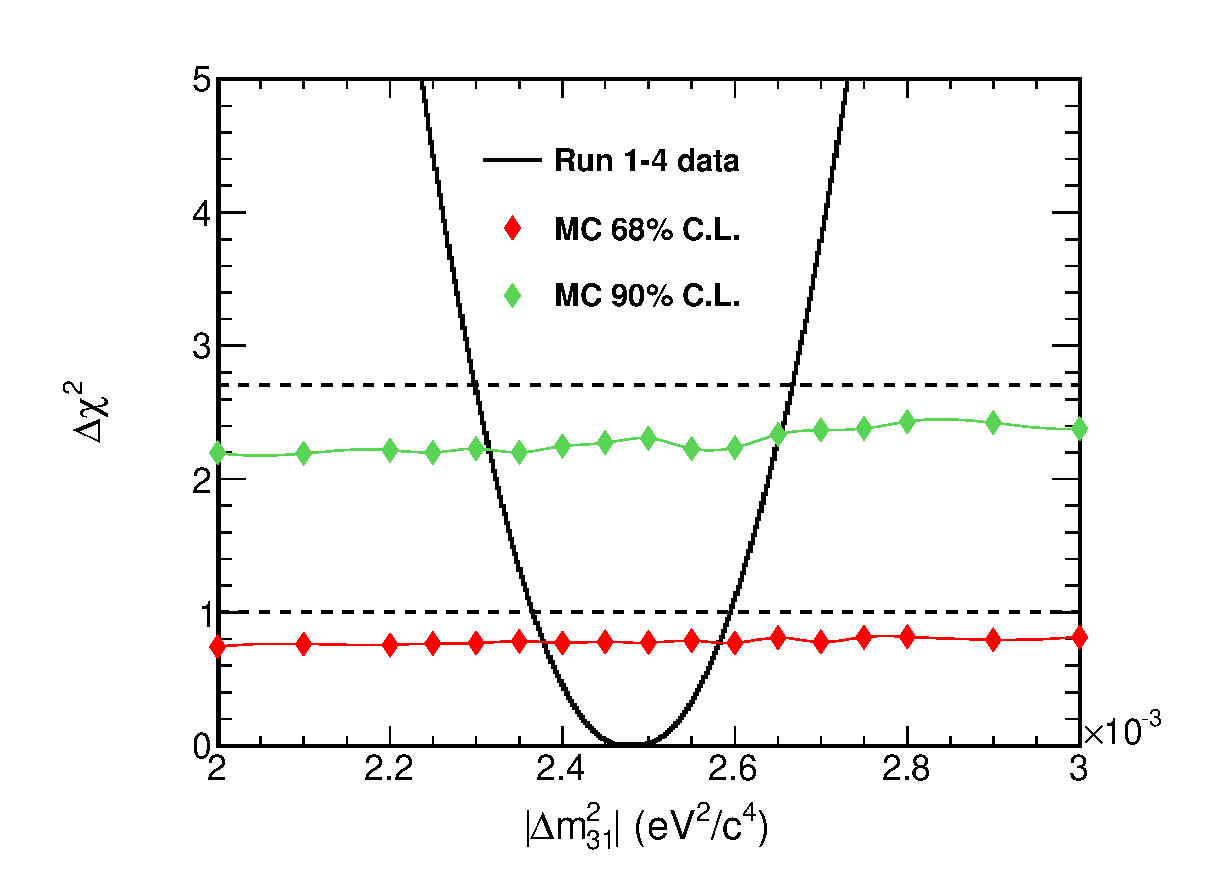
\includegraphics[width=30pc]{./images/data_fit/inverted31/run1-4_nuis4_dm31sq_inverted_1DFC_interval}
    \caption {
     Comparison between the 1D $\Delta \chi^{2}$ from the fit of the Run 1+2+3+4 data and the Monte Carlo estimation of the
     1D 68\% and 90\% critical values of $\Delta \chi^{2}$ as a function of $|\Delta m^{2}_{31}|$. Each MC
     critical value is obtained from 10000 toy experiments with systematic variations and statistical fluctuations; these
     critical values are fitted with cubic splines. The inverted mass hierarchy is assumed.
     The canonical constant-$\Delta \chi^{2}$ 68\% and 90\% critical values for one degree of freedom are shown as dashed lines.
    }
    \label{fig:results_1D_dchisq_dm32sq_inverted}
  \end{minipage}
\end{figure*}

\begin{table}[htb]
  \centering
  \begin{tabular}{| c | c | c | c | D{.}{.}{-1} D{.}{.}{-1} | D{.}{.}{-1}  D{.}{.}{-1} |}
    \hline
    Method  & Dataset & Mass  & Confidence & \multicolumn{2}{c|}{$\sin^{2}\theta_{23}$}
    &  \multicolumn{2}{c|}{$|\Delta m^{2}_{32}|$ or $|\Delta m^{2}_{31}|$}  \\
    & & hierarchy & level  & \multicolumn{2}{c|}{} &  \multicolumn{2}{c|}{(10$^{-3}$ eV$^2$/c$^4$)} \\
    \hline
    \hline
    \multirow{4}{*}{Constant $\Delta\chi^2$} & \multirow{4}{*}{Run 1+2+3+4} & \multirow{2}{*}{Normal} & 68\% & \multicolumn{2}{c|}{\resultNormalMixingErrorsShort} & \multicolumn{2}{c|}{\resultNormalDmsqErrorsShort} \\
    \cline{4-8}
                                             & &             & 90\% & \multicolumn{2}{c|}{\resultNormalMixingTwoSigmaLo \: $<$ $\sin^{2}\theta_{23}$ $<$ \resultNormalMixingTwoSigmaHi}
                                             & \multicolumn{2}{c|}{\resultNormalDmsqTwoSigmaLo \: $<$ $|\Delta m^{2}_{32}|$ $<$ \resultNormalDmsqTwoSigmaHi} \\
    \cline{3-8}
                                             & & \multirow{2}{*}{Inverted} & 68\% & \multicolumn{2}{c|}{\resultInvertedMixingErrorsShort} & \multicolumn{2}{c|}{\resultInvertedDmsqErrorsShort} \\
    \cline{4-8}
                                             & &             & 90\% & \multicolumn{2}{c|}{\resultInvertedMixingTwoSigmaLo \: $<$ $\sin^{2}\theta_{23}$ $<$ \resultInvertedMixingTwoSigmaHi}
                                             & \multicolumn{2}{c|}{\resultInvertedDmsqTwoSigmaLo \: $<$ $|\Delta m^{2}_{31}|$ $<$ \resultInvertedDmsqTwoSigmaHi} \\
    \hline
                                             & \multirow{4}{*}{Run 1+2+3+4} & \multirow{2}{*}{Normal} & 68\% & \multicolumn{2}{c|}{\resultNormalMixingFCErrorsShort} & \multicolumn{2}{c|}{\resultNormalDmsqFCErrorsShort} \\
    \cline{4-8}
    Feldman \&                               & &             & 90\% & \multicolumn{2}{c|}{\resultNormalMixingTwoSigmaFCLo \: $<$ $\sin^{2}\theta_{23}$ $<$ \resultNormalMixingTwoSigmaFCHi}
                                             & \multicolumn{2}{c|}{\resultNormalDmsqTwoSigmaFCLo \: $<$ $|\Delta m^{2}_{32}|$ $<$ \resultNormalDmsqTwoSigmaFCHi} \\
    \cline{3-8}
    Cousins
    & & \multirow{2}{*}{Inverted} & 68\% & \multicolumn{2}{c|}{\resultInvertedMixingFCErrorsShort} & \multicolumn{2}{c|}{\resultInvertedDmsqFCErrorsShort} \\
    \cline{4-8}
                                             & &             & 90\% & \multicolumn{2}{c|}{\resultInvertedMixingTwoSigmaFCLo \: $<$ $\sin^{2}\theta_{23}$ $<$ \resultInvertedMixingTwoSigmaFCHi}
                                             & \multicolumn{2}{c|}{\resultInvertedDmsqTwoSigmaFCLo \: $<$ $|\Delta m^{2}_{31}|$ $<$ \resultInvertedDmsqTwoSigmaFCHi} \\
    \hline
    \hline
    \multirow{2}{*}{Constant $\Delta\chi^2$} & \multirow{2}{*}{Run 1+2+3} & \multirow{2}{*}{Normal} & 68\% &
                          \multicolumn{2}{c|}{\resultNormalRunITIIIMixingErrorsShort} & \multicolumn{2}{c|}{\resultNormalRunITIIIDmsqErrorsShort} \\
    \cline{4-8}
                                             & &             & 90\% & \multicolumn{2}{c|}{\resultNormalRunITIIIMixingTwoSigmaLo \: $<$ $\sin^{2}\theta_{23}$ $<$ \resultNormalRunITIIIMixingTwoSigmaHi}
                                             & \multicolumn{2}{c|}{\resultNormalRunITIIIDmsqTwoSigmaLo \: $<$ $|\Delta m^{2}_{32}|$ $<$ \resultNormalRunITIIIDmsqTwoSigmaHi} \\
    \hline
    \multirow{2}{*}{Constant $\Delta\chi^2$} & \multirow{2}{*}{Run 4} & \multirow{2}{*}{Normal} & 68\% &
                          \multicolumn{2}{c|}{\resultNormalRunIVMixingErrorsShort} & \multicolumn{2}{c|}{\resultNormalRunIVDmsqErrorsShort} \\
    \cline{4-8}
                                             & &             & 90\% & \multicolumn{2}{c|}{\resultNormalRunIVMixingTwoSigmaLo \: $<$ $\sin^{2}\theta_{23}$ $<$ \resultNormalRunIVMixingTwoSigmaHi}
                                             & \multicolumn{2}{c|}{\resultNormalRunIVDmsqTwoSigmaLo \: $<$ $|\Delta m^{2}_{32}|$ $<$ \resultNormalRunIVDmsqTwoSigmaHi} \\
    \hline
  \end{tabular}
  \caption{
    Summary of one-dimensional limits on $\sin^{2}\theta_{23}$ and $|\Delta m^{2}_{32}|$ or
    $|\Delta m^{2}_{31}|$ from the fits of the Run 1+2+3, Run 4, and Run 1+2+3+4 datasets.
    The limits are shown for both the constant-$\Delta\chi^2$ method and the new procedure
    described in Sec.\ \ref{sec:contour_construction}.
   }
  \label{tab:data_fits:1dlimits}
\end{table}

\clearpage

%--------------------------------------------------------------------------------------
% Contour comparisons
%--------------------------------------------------------------------------------------

\subsection {Comparisons of confidence regions}
\label{sec:results_contour_comparisons}

A comparison is shown in Fig.\ \ref{fig:results_compare_normal_inverted:constdchisq}
between the Run 1+2+3+4 2-dimensional confidence regions for the normal and inverted mass hierarchies  
obtained using the constant-$\Delta\chi^2$ method (the vertical axis is $|\Delta m_{32}^{2}|$ for the normal mass hierarchy and 
$|\Delta m_{31}^{2}|$ for the inverted mass hierarchy). The equivalent comparison between confidence regions for the two mass 
hierarchies obtained using the Feldman-Cousins method is shown in Fig.\ \ref{fig:results_compare_normal_inverted:fc}.

The Run 1+2+3+4 2-dimensional confidence regions obtained using the constant-$\Delta\chi^2$ and Feldman-Cousins methods
are compared in Fig.\ \ref{fig:results_compare_FC_constdchisq:normal} for the normal mass hierarchy and 
Fig.\ \ref{fig:results_compare_FC_constdchisq:inverted} for the inverted mass hierarchy.
The Feldman-Cousins confidence regions are narrower along $|\Delta{m^{2}_{32}}|$ or $|\Delta{m^{2}_{31}}|$ at maximal disappearance than
those made with the constant-$\Delta\chi^{2}$ method since the Feldman-Cousins $\Delta\chi^2_{critical}$ values are lower 
than the canonical constant-$\Delta\chi^2$ values as explained in Sec.\ \ref{sec:results_contours}. This narrowing of the 
2-dimensional confidence contour was also seen in our earlier Run 1+2 and Run 1+2+3 analyses 
\cite{OurRun12DisappAnalysis,OurRun123DisappAnalysis3Flavour} in which we fitted 
$\sin^{2}{2\theta_{23}}$ instead of $\sin^{2}{\theta_{23}}$. In this analysis, the Feldman-Cousins contours are also 
very slightly narrower in $\sin^{2}{\theta_{23}}$ for values of $|\Delta{m^{2}_{32}}|$ or $|\Delta{m^{2}_{31}}|$ near the best fit.

In Figs.\ \ref{fig:results_compare_FC_constdchisq_external} and \ref{fig:results_compare_FC_constdchisq_external_inverted},
the T2K Run 1+2+3+4 90\% confidence region is compared with 
those from MINOS (2013) \cite{MINOS2013sinsqtheta}, SuperK atmospherics 
(2013 3-flavour 
zenith-angle analysis) \cite{SKAtm2012},
and T2K Run 1+2+3 \cite{T2KRun123Disapp}, for the normal and inverted hierarchies respectively.
A second comparison with external results is shown in Fig.\ \ref{fig:results_compare_FC_constdchisq_external_sinsqtheta23}: 
this figure compares the T2K Run 1+2+3+4 90\% confidence region with
those from MINOS (2013) \cite{MINOS2013}, SuperK atmospherics 
(2012 2-flavour L/E and 3-flavour 
zenith-angle analyses) \cite{SKAtm2012},
and T2K Run 1+2+3 \cite{T2KRun123Disapp},
for the normal mass hierarchy only.
In this plot, the T2K Run 1+2+3+4 fit result has been converted from $\sin^2\theta_{23}$ to
$\sin^2(2\theta_{23})$ by profiling the octant.
This is the same method as that used by SuperK in their zenith angle contour, and,
if this method had been applied to the T2K Run 1+2+3 result, it should have
closely matched the T2K Run 1+2+3 $\theta_{23} \geq \pi/4$ contour.
These plots show that T2K now has the world's best limit in $\theta_{23}$.

In Fig.\ \ref{fig:results_compare_constdchisq_sensitivity_normal}
a comparison is shown
between the Run 1+2+3+4 allowed region obtained 
with constant-$\Delta\chi^{2}$ method and the T2K 6.5700$\times$10$^{20}$ POT sensitivity
contour produced at our best-fit point for the Run 1+2+3+4 dataset.
The 'stat-only' sensitivity contours were computed by averaging the contours of 300 toy MC
experiments generated with statistical fluctuations and all systematic parameters fixed at
their nominal values.
The 'stat+syst' sensitivity contours were computed by averaging the contours of 300 toy MC
experiments generated with statistical fluctuations and all systematic parameters randomized.
As can be seen in the the plot, the T2K data results in a smaller contour than the sensitivity,
particularly for the $\sin^2\theta_{23}$ limit.
p-values can be calculated by comparing the data constant-$\Delta\chi^2$ limits
with the limits of the 'stat+syst' sensitivity fits, and represent the fraction of toy experiments that  provide a \emph{tighter} limit than the data.
For $\sin^2\theta_{23}$ the p-values are 0.21(0.19) for 68\% C.L. and 0.19(0.21) for 90\% C.L. for the lower(upper) limits respectively.
For $|\Delta m^2_{32}|$ the p-values are 0.31(0.20) for 68\% C.L. and 0.42(0.27) for 90\% C.L. for the lower(upper) limit respectively.
This shows that the data are not an extreme fluctuation.
% {\color{red} why not FC? - area is bigger than the surface we have}.

Finally, a comparison between the confidence regions obtained by three 
separate analyses of the Run 1+2+3+4, Run 1+2+3 and Run 4 datasets 
is shown in Fig.\ \ref{fig:results_compare_runs}.
The contours from the different running periods are consistent.

% ......................
% 
% const Delta & FC \chisq normal vs inverted
% 
\begin{figure*}[htb]
  \center
  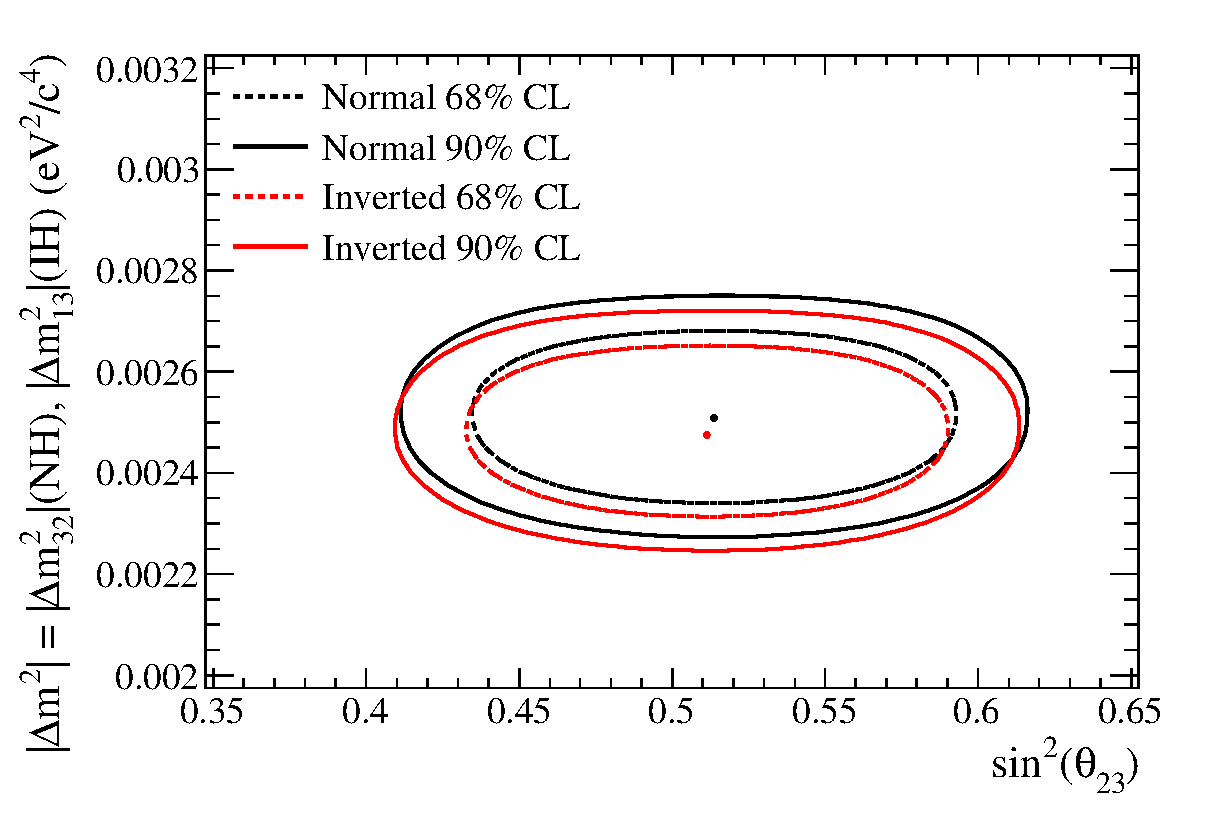
\includegraphics[width=30pc]{./images/data_fit/compare/contours_run1-4_nuis4_hierarchy}
  \caption {
    Comparison between the 68\% CL and 90\% CL allowed regions 
    for the normal and inverted mass hierarchies
    obtained using the constant-$\Delta\chi^2$ method
    from the fit of the Run 1+2+3+4 dataset.
  }
  \label{fig:results_compare_normal_inverted:constdchisq}
\end{figure*}

\begin{figure*}[htb]
  \center
  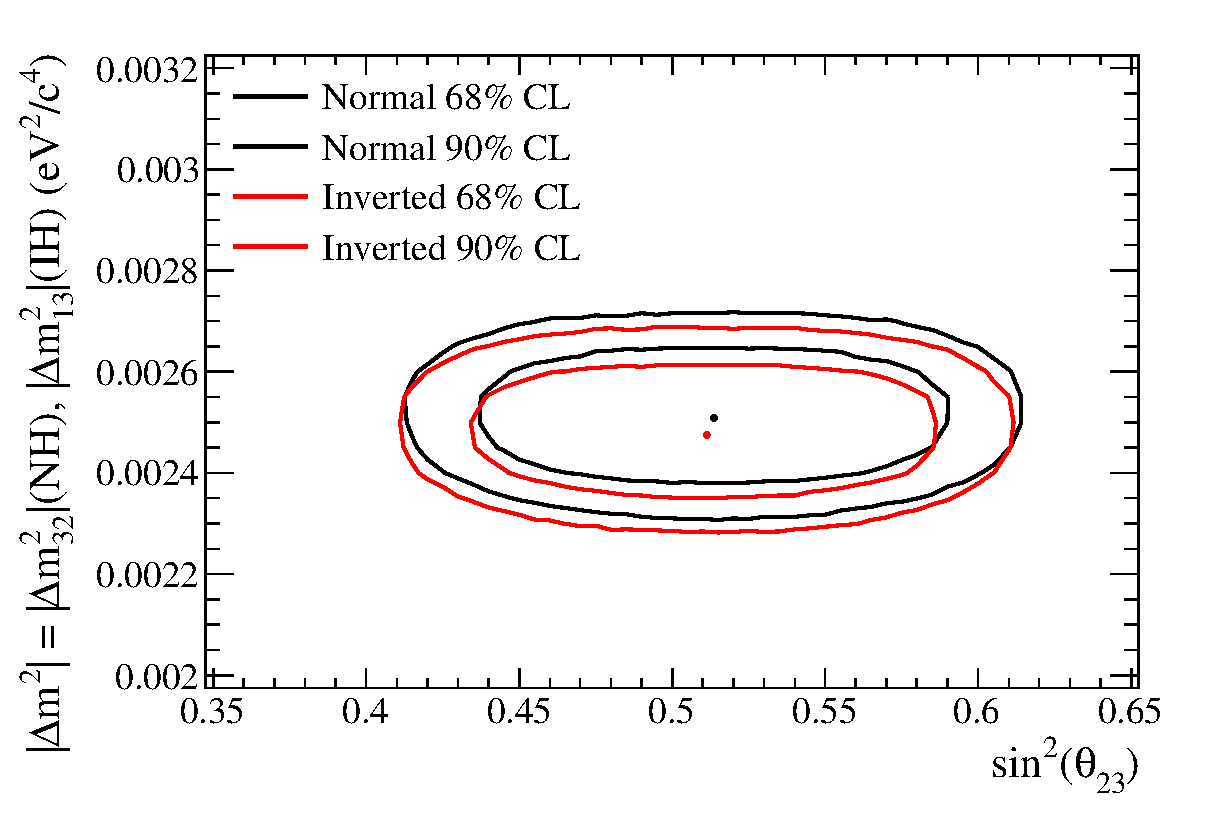
\includegraphics[width=30pc]{./images/data_fit/fc/contour_compare_hierarchies_fc}
  \caption {
    Comparison between the 68\% CL and 90\% CL allowed regions 
    for the normal and inverted mass hierarchies
    obtained using the Feldman-Cousins method
    from the fit of the Run 1+2+3+4 dataset.
  }
  \label{fig:results_compare_normal_inverted:fc}
\end{figure*}

% ......................
% 
% const Delta\chisq vs FC (normal and inverted)
% 
\begin{figure*}[htb]
  \center
  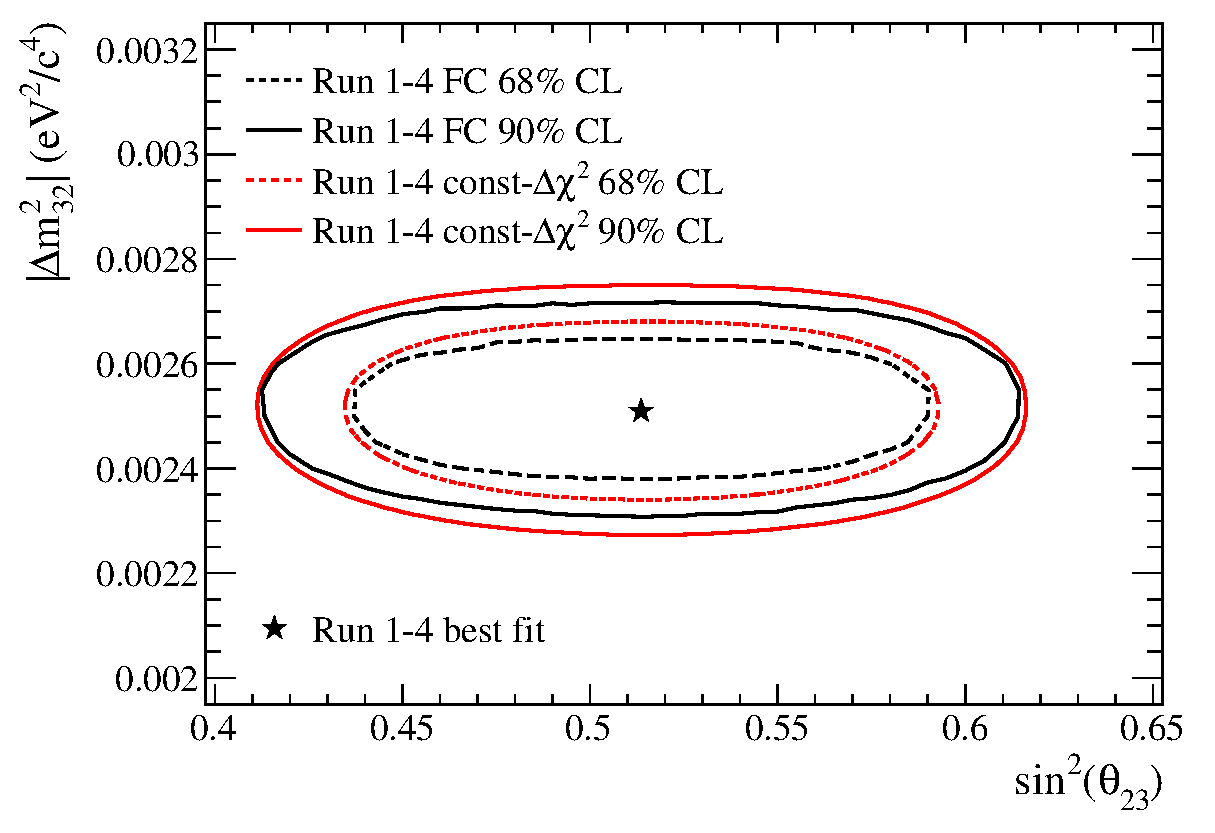
\includegraphics[width=30pc]{./images/data_fit/fc/contour_compare_normal_dcvsfc}
  \caption {
    Comparison between the 68\% CL and 90\% CL allowed regions 
    obtained using the constant-$\Delta\chi^2$ and Feldman-Cousins methods 
    from the fit of the Run 1+2+3+4 dataset.
    The normal mass hierarchy is assumed.
  }
  \label{fig:results_compare_FC_constdchisq:normal}
\end{figure*}

\begin{figure*}[htb]
  \center
  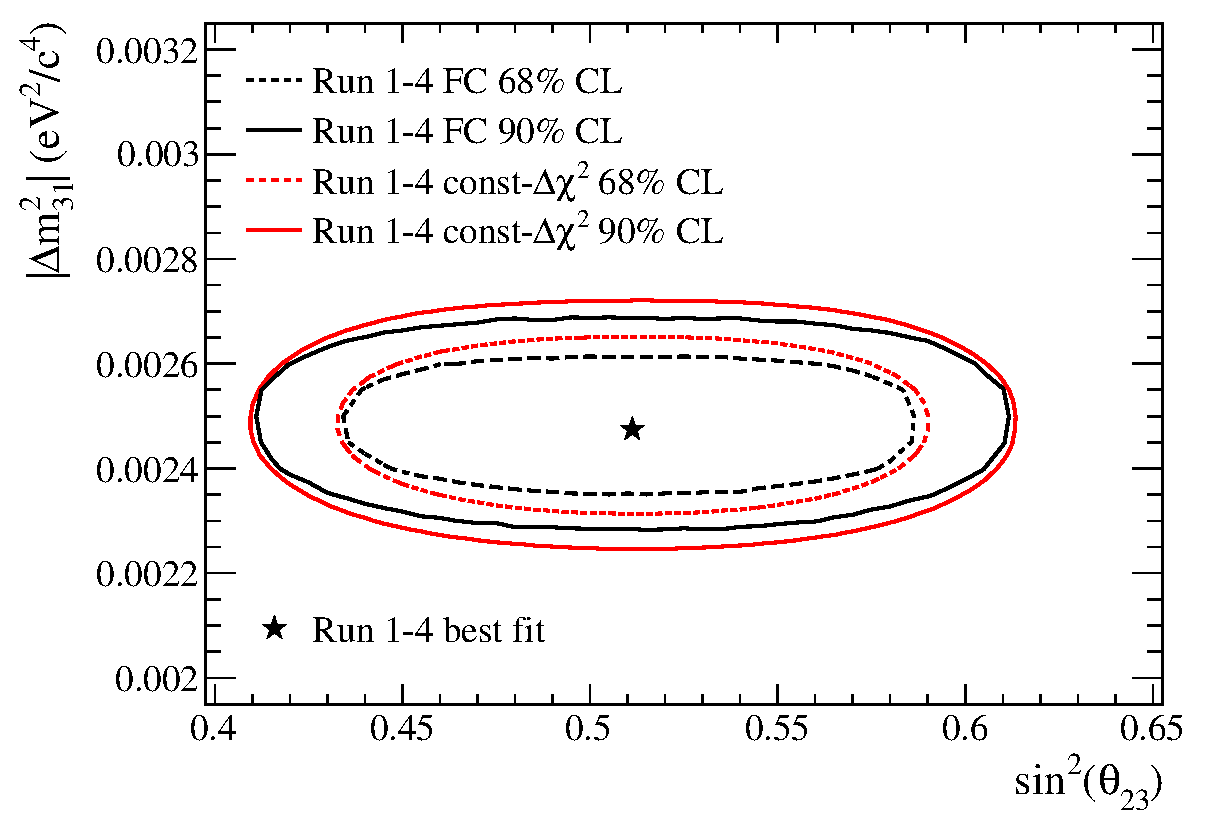
\includegraphics[width=30pc]{./images/data_fit/fc/contour_compare_inverted31_dcvsfc}
  \caption {
    Comparison between the 68\% CL and 90\% CL allowed regions 
    obtained using the constant-$\Delta\chi^2$ and Feldman-Cousins methods 
    from the fit to the Run 1+2+3+4 dataset.
    The inverted mass hierarchy is assumed.
  }
  \label{fig:results_compare_FC_constdchisq:inverted}
\end{figure*}


%......................
%
% VALOR vs the world
% 
\begin{figure*}[htb]
  \center
  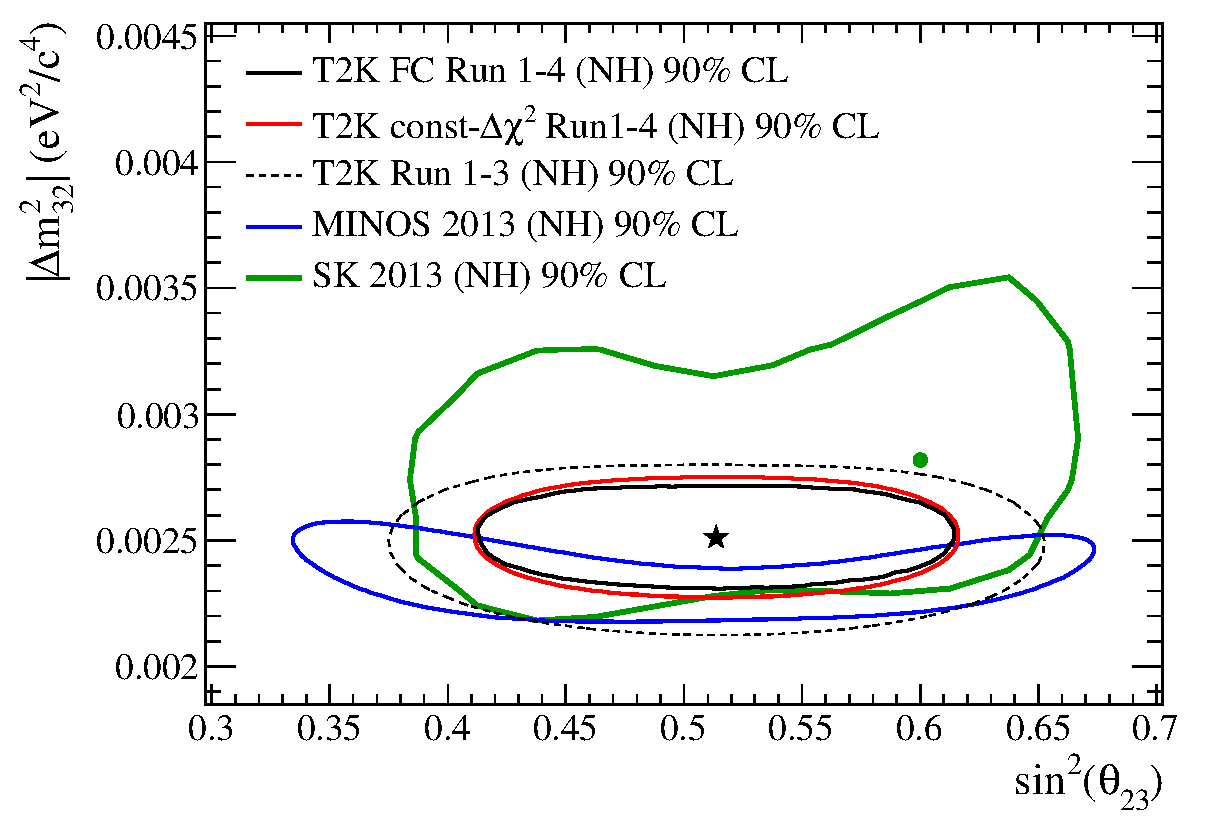
\includegraphics[width=30pc]{./images/data_fit/fc/contour_compare_normal_dcvsfc_ext}
  \caption {
    Comparison between 90\% CL allowed regions 
    from MINOS \cite{MINOS2013sinsqtheta}, SuperK atmospherics \cite{SKAtm2012}, T2K Run 1+2+3 \cite{T2KRun123Disapp},
    and the 90\% CL region obtained from the {\em VALOR} fit of the Run 1+2+3+4 dataset.
    Contours obtained using both the constant-$\Delta\chi^2$ and Feldman-Cousins methods are shown.
    The normal mass hierarchy is assumed for all results.
  }
  \label{fig:results_compare_FC_constdchisq_external}
\end{figure*}

\begin{figure*}[htb]
  \center
  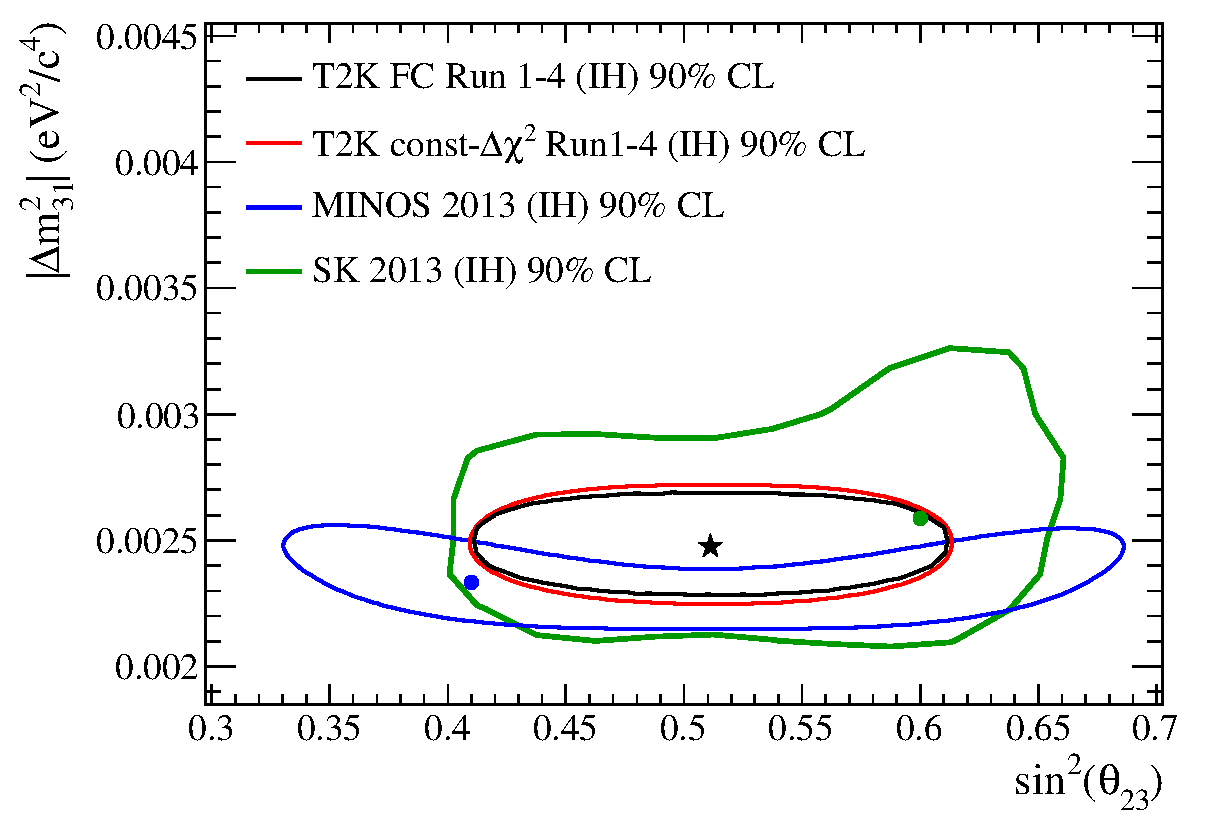
\includegraphics[width=30pc]{./images/data_fit/fc/contour_compare_inverted31_dcvsfc_ext}
  \caption {
    Comparison between 90\% CL allowed regions 
    from MINOS \cite{MINOS2013sinsqtheta}, SuperK atmospherics \cite{SKAtm2012}, T2K Run 1+2+3 \cite{T2KRun123Disapp},
    and the 90\% CL region obtained from the {\em VALOR} fit of the Run 1+2+3+4 dataset.
    Contours obtained using both the constant-$\Delta\chi^2$ and Feldman-Cousins methods are shown.
    The inverted mass hierarchy is assumed for all results.
  }
  \label{fig:results_compare_FC_constdchisq_external_inverted}
\end{figure*}

\begin{figure*}[htb]
  \center
  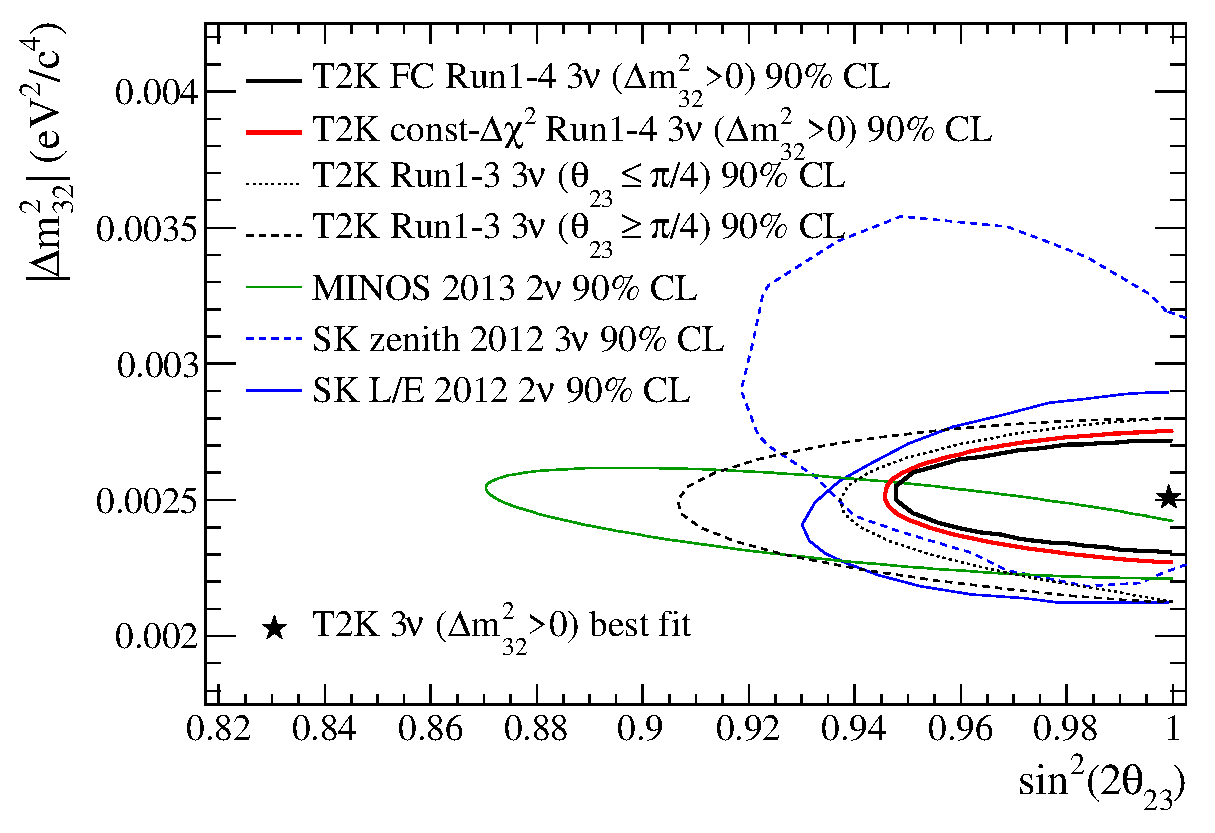
\includegraphics[width=30pc]{./images/data_fit/fc/contour_compare_constdchisqfc_external_sinsq2theta23}
  \caption {
    Comparison between 90\% CL allowed regions 
    from MINOS \cite{MINOS2013}, SuperK atmospherics \cite{SKAtm2012}, T2K Run 1+2+3 \cite{T2KRun123Disapp},
    and the 90\% CL region obtained from the {\em VALOR} fit of the Run 1+2+3+4 dataset.
    Contours obtained using both the constant-$\Delta\chi^2$ and Feldman-Cousins methods are shown.
    The normal mass hierarchy is assumed for all results.
  }
  \label{fig:results_compare_FC_constdchisq_external_sinsqtheta23}
\end{figure*}

% ......................
% 
% Comparison with sensitivity
% 
\begin{figure*}[htb]
  \center
  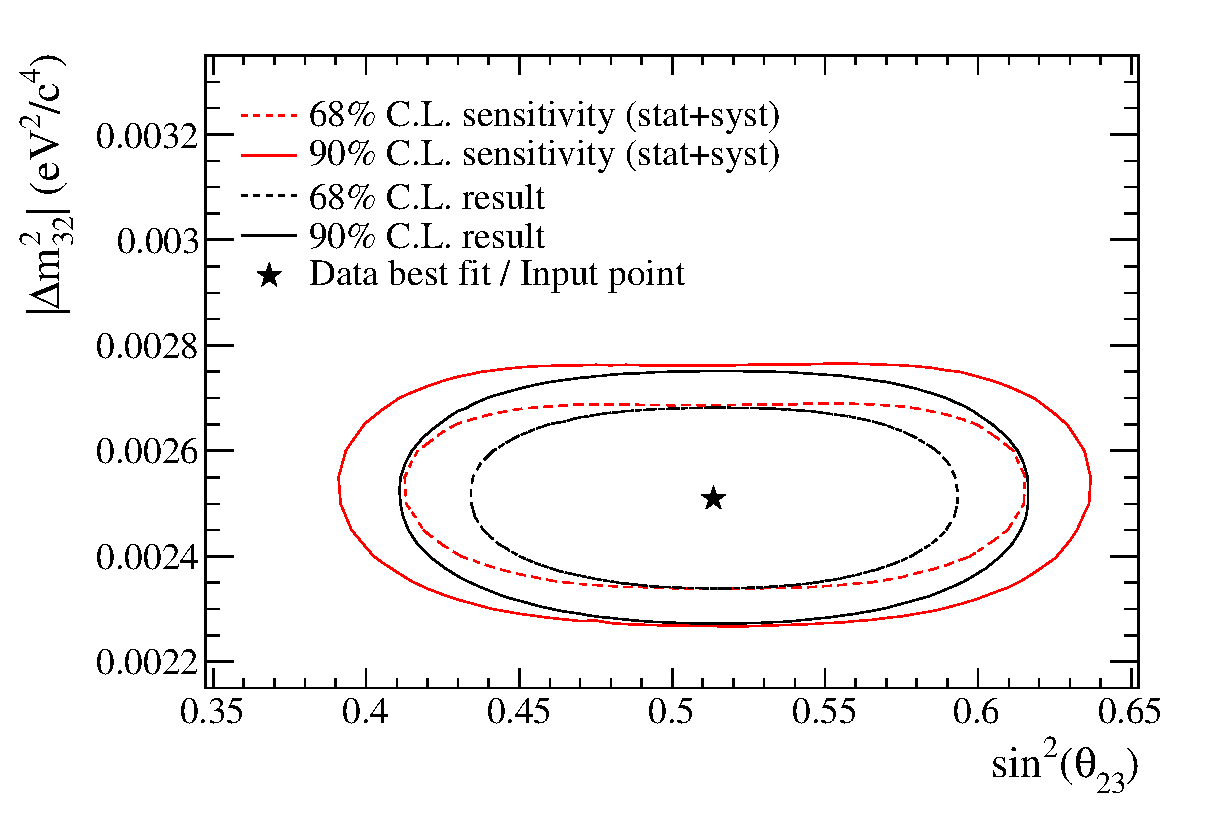
\includegraphics[width=30pc]{./images/data_fit/sensitivity/sensitivity_normal}
  \caption {
    Comparison between the 68\% CL and 90\% CL allowed regions using the constant-$\Delta\chi^2$ 
    method from the fit of the Run 1+2+3+4 dataset
    and the results of
    % sensitivity studies
    a sensitivity study
    at the best-fit point for Run 1+2+3+4
    for
    %both statistical-only and
    statistical+systematic MC toys.
    The normal mass hierarchy is assumed.
  }
  \label{fig:results_compare_constdchisq_sensitivity_normal}
\end{figure*}

% ......................
% 
% Run 1+2+3+4 vs Run 1+2+3 vs Run 4
% 
\begin{figure*}[htb]
  \center
  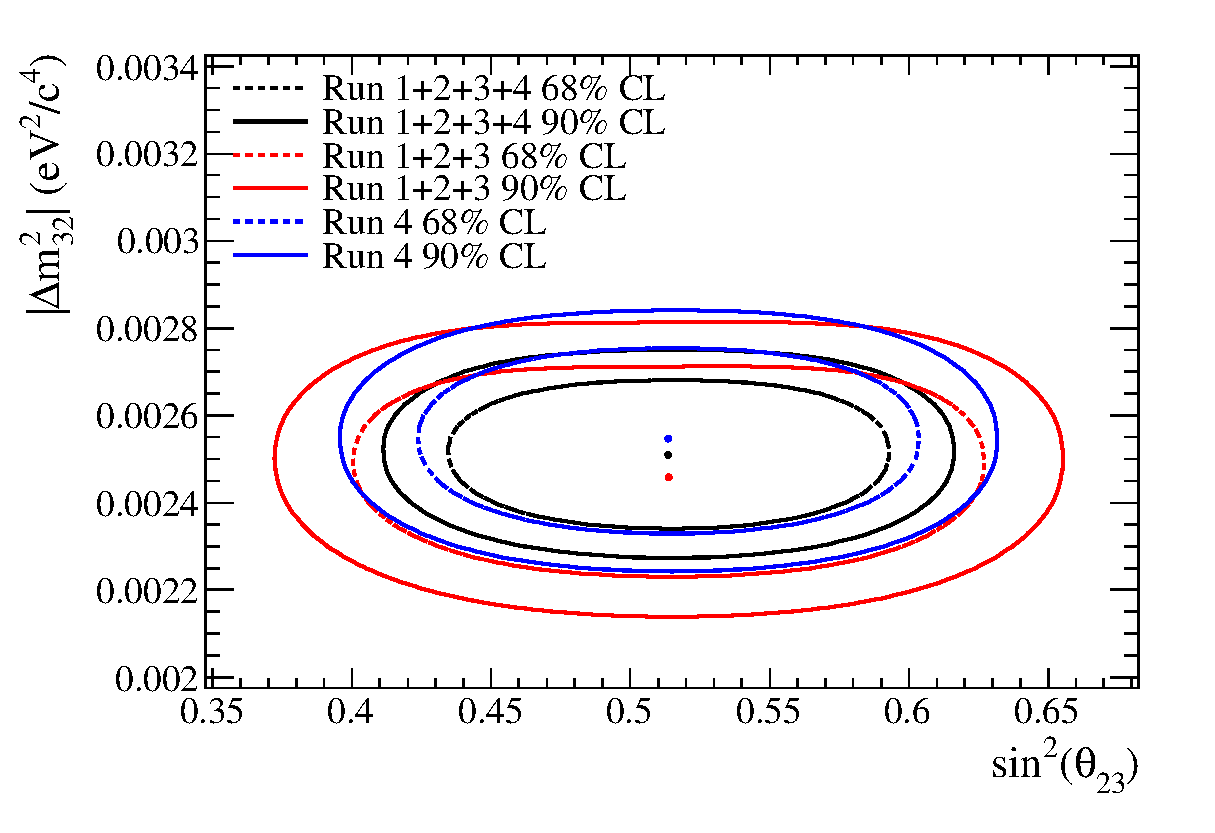
\includegraphics[width=30pc]{./images/data_fit/compare/contours_run1-4_nuis4_sepruns}
  \caption {
  Comparison between the 68\% CL and 90\% CL allowed regions obtained from separate
  analyses to the Run 1+2+3+4, Run 1+2+3 and Run 4 datasets.
  All contours shown were calculated with the constant-$\Delta\chi^2$ method.
  The normal mass hierarchy is assumed.
}
  \label{fig:results_compare_runs}
\end{figure*}


% \clearpage

